\section{Groups}
\subsection{Semi-groups, Monoids and Groups}
If $G$ is a nonempty set, then we can define a \textbf{binary operation} on $G$, which is a function $G\times G\to G$. For example, $a+b,a\cdot b$(additive notation and multiplicative notation) are all binary operations. For convenience we shall always use the multiplicative notation in this chapter.
\begin{definition}
A \textbf{semi-group} is a nonempty set $G$ together with a binary operation $\cdot$ which is:\par
(i)associative:\ $a(bc)=(ab)c$ for all $a,b,c\in G$;\par
A \textbf{monoid} is a semi-group which contains a
(ii)(two sided) identity element $e\in G$ such that $ae=ea=a$ for all $a\in G$;\par
A \textbf{group} is a monoid $G$ such that 
(iii)for all $a\in G$ there exists a (two sided) inverse element $a^{-1}\in G$ such that $a^{-1}a=aa^{-1}=e$.
\end{definition}
It is trivial to proof that the identity and the inverse in a group is unique. We skip the proof. We can also define the \textbf{order} of a group $|G|$ as the cardinal of $G$. We say a group is abelian, if its binary operation is commutative, which is $ab=ba$ for all $a,b\in G$.\par
The following proposition shows that the axioms that defined a group may be weakened:
\begin{proposition}
Let $G$ be a semi-group. Then $G$ is a group if and only if:\par
(i)there exists a left identity element $e$ such that $ea=a$ for all $a\in G$;\par
(ii)there exists a left inverse element $a^{-1}$ such that $a^{-1}a=e$ for all $a\in G$.\par
\end{proposition}
\begin{proof}
$\Rightarrow$:Trivial.\par
$\Leftarrow$:We proof the existence of right identity and right inverse element. In fact, observed that
$$(aa^{-1})(aa^{-1})=a(a^{-1}a)a^{-1}=aea^{-1}=aa^{-1}$$
and for all $c\in G$ we have 
$$cc=c\Rightarrow c^{-1}cc=c^{-1}c\Rightarrow ec=e\Rightarrow c=e,$$
hence 
$$aa^{-1}=(aa^{-1})^{-1}(aa^{-1})=e,$$
and 
$$ae=a(a^{-1}a)=(aa^{-1})a=ea=a,$$
we know by the definition of group that $G$ is a group. 
\end{proof}
\begin{proposition}
Let $G$ be a semi-group. Then $G$ is a group if and only if for all $a,b\in G$ the equations $ax=b$ and $ya=b$ has solutions in $G$.
\end{proposition}
\begin{proof}
$\Rightarrow$:Trivial.\par
$\Leftarrow$:We first proof that there exists left identity in $G$. For all $a\in G$, the equation $xa=a$ has solutions, we denote as $e$. Now for all $b\in G$, we have 
$$b=ax=eax=eb,$$
which shows that $e$ is the left identity of $G$. Then since the equation $xa=e$ has solutions, hence for all $a\in G$ there exists left inverse. By proposition 2.2 we know that $G$ is a group.
\end{proof}
We give some examples.
\begin{example}\em
Consider a square with vertices numbered $1,2,3$ and $4$, center at the origin and sides parallel to the axes:
\begin{center}
\tikzset{every picture/.style={line width=0.75pt}} %set default line width to 0.75pt        

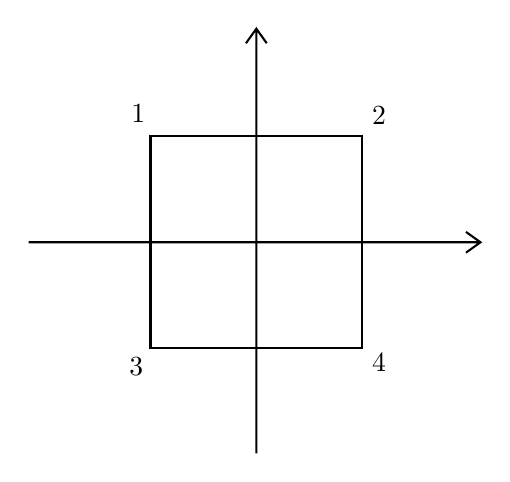
\begin{tikzpicture}[x=0.75pt,y=0.75pt,yscale=-1,xscale=1]
%uncomment if require: \path (0,476); %set diagram left start at 0, and has height of 476

%Shape: Axis 2D [id:dp5301733644862636] 
\draw  (202,196.89) -- (419.67,196.89)(311.67,94) -- (311.67,298.55) (412.67,191.89) -- (419.67,196.89) -- (412.67,201.89) (306.67,101) -- (311.67,94) -- (316.67,101)  ;
%Shape: Square [id:dp9849820568686898] 
\draw   (260.67,145.89) -- (362.67,145.89) -- (362.67,247.89) -- (260.67,247.89) -- cycle ;

% Text Node
\draw (250,128.89) node [anchor=north west][inner sep=0.75pt]   [align=left] {1};
% Text Node
\draw (366,129.89) node [anchor=north west][inner sep=0.75pt]   [align=left] {2};
% Text Node
\draw (249,250.89) node [anchor=north west][inner sep=0.75pt]   [align=left] {3};
% Text Node
\draw (366,248.89) node [anchor=north west][inner sep=0.75pt]   [align=left] {4};
\end{tikzpicture}
\end{center}
Let $D_4^*$ be the following set of transformations of the square:
$$D_4^*=\{R,R_2,R_3,I,T_x,T_y,T_{13},T_{24}\},$$
where $R$ means a $90^\circ$ rotation counter-clockwise, $R_2$ means a $180^\circ$ rotation counter-clockwise and so on, $I$ means a $360^\circ$ rotation counter-clockwise. $T_x$ is a reflection about the $x$-axis, $T_y$ is a reflection about the $y$-axis, $T_{13}$ and $T_{24}$ are reflections about $y=-x$ and $y=x$. Define a binary operation on $D_4^*$ to be composition of transformations, then $D_4^*$ is a group, which is called the \textbf{group of symmetries of the square}.
\end{example}
\begin{example}\em
Let $S$ be a nonempty set and $A(S)$ the set of all bijections $S\to S$. Under the operation of composition of functions, $A(S)$ is a group, it is called the \textbf{group of permutations on the set $S$}, and the elements of $A(S)$ are called \textbf{permutations}. If $S=\{1,2,\cdots,n\}$, then $A(S)$ is called the \textbf{symmetric group on n letters} and denoted as $S_n$. For any $\sigma\in S_n$, we may denote it as a chart $\sigma =\left( \begin{matrix}
	1&		2&		\cdots&		n\\
	i_1&		i_2&		\cdots&		i_n\\
\end{matrix} \right) $. For example, in $S_4$, let 
$$
\sigma =\left( \begin{matrix}
	1&		2&		3&		4\\
	3&		1&		2&		4\\
\end{matrix} \right) \,\,\text{and}\, \tau =\left( \begin{matrix}
	1&		2&		3&		4\\
	4&		1&		2&		3\\
\end{matrix} \right) ,
$$
then 
$$
\sigma \tau =\left( \begin{matrix}
	1&		2&		3&		4\\
	3&		1&		2&		4\\
\end{matrix} \right) \left( \begin{matrix}
	1&		2&		3&		4\\
	4&		1&		2&		3\\
\end{matrix} \right) =\left( \begin{matrix}
	1&		2&		3&		4\\
	4&		3&		1&		2\\
\end{matrix} \right) 
$$
and
$$
\tau \sigma =\left( \begin{matrix}
	1&		2&		3&		4\\
	4&		1&		2&		3\\
\end{matrix} \right) \left( \begin{matrix}
	1&		2&		3&		4\\
	3&		1&		2&		4\\
\end{matrix} \right) =\left( \begin{matrix}
	1&		2&		3&		4\\
	2&		4&		1&		3\\
\end{matrix} \right) ,
$$
which also states that $S_n$ may not be abelian.
\end{example}
\begin{example}\em
We may construct new groups with old groups. For example, let $G$ and $H$ be groups with binary operations, define $G\times H$ with binary operation
$$(a,b)(a^\prime,b^\prime)=(aa^\prime,bb^\prime),\text{where}\ a,a^\prime\in G,b,b^\prime\in H,$$
then $G\times H$ is a group. If $G$ and $H$ were abelian, then $G\times H$ is abelian.
\end{example}
\begin{theorem}
Let $R(\sim)$ be an equivalence relation on a monoid $G$ such that $a_1\sim a_2$ and $b_1\sim b_2$ implies $a_1a_2\sim b_1b_2$ for all $a_i,b_i\in G,i=1,2$.Then $G/R$ is a monoid under the binary operation $\overline{a}\overline{b}=\overline{ab}$. If $G$ is an (abelian) group, then so is $G/R$.
\end{theorem}
\begin{proof}
We first proof that $G/R$ is well-defined. For $\overline{a_1}=\overline{a_2},\overline{b_1}=\overline{b_2}$ we have $a_1\sim a_2$ and $b_1\sim b_2$, and hence $a_1a_2\sim b_1b_2$, which is $\overline{a_1a_2}=\overline{b_1b_2}$. Next we verify $G/R$ is a monoid by definition. First,
$$
\overline{a}\left( \overline{b}\overline{c} \right) =\overline{a}\left( \overline{bc} \right) =\overline{abc},\left( \overline{a}\overline{b} \right) \overline{c}=\left( \overline{ab} \right) \overline{c}=\overline{abc},
$$
hence $G/R$ is associative. Then since $G$ is a monoid, then there exists $e\in G$ such that $e$ is the identity element of $G$. It is easy to verify that $\overline{e}$ is the identity element of $G/R$, which finished our proof.\par
If $G$ is a group, then it is trivial that for all $\overline{a}\in G/R$, $\overline{a^{-1}}$ is the inverse of $\overline{a}$, and if $G$ is abelian, then so is $G/R$.
\end{proof}
An equivalence relation on a monoid $G$ that satisfies the hypothesis above is called a \textbf{congruence relation} on $G$.
\begin{example}\em
Let $m$ be a fixed integer. Then congruence modulo $m$, denote as $\sim$, is a congruence relation. By theorem 2.4 we know that $\mathbb{Z}/\sim$(with additive notation) is an abelian group, we denote as $\mathbb{Z}_m$ and call it \textbf{group of integers modulo $m$}.
\end{example}
\begin{example}\em
The following relation on the additive group $\mathbb{Q}$ of rational numbers is a congruence relation:
$$a\sim b\Leftrightarrow a-b\in\mathbb{Z},$$
which will be proved in exercises. By Theorem 2.4 we know that the equivalence class(denoted as $\mathbb{Q}/\mathbb{Z}$) is an abelian group with infinite order. $\mathbb{Q}/\mathbb{Z}$ is called the \textbf{group of rationals modulo one}.
\end{example}
Next we discuss the product of a number of elements $a_1,a_2,\cdots$ in a semi-group. We may define the \textbf{meaningful product}(denote as $\prod_{i}a_i$) by induction: for one element $a_1$, the product is clearly $a_1$. Then for all $n>2$, we may denote the product of $a_1,a_2,\cdots,a_n$ as $\prod_{i=1}^na_i=\left(\prod_{i=1}^{n-1}a_i\right)a_n$.
\begin{theorem}
If $G$ is a semi-group and $a_1,a_2,\cdots,a_n\in G$, then any two meaningful products of $a_1,a_2,\cdots,a_n$ in this order are equal.
\end{theorem}
\begin{proof}
We proof by induction. For $n=1,2$, the statement is trivially true. For $m>2$, if $a_1a_2\cdots a_n=\left( a_1\cdots a_m \right) \left( a_{m+1}\cdots a_n \right) $, then we have 
$$
a_1a_2\cdots a_n=\left( \prod_{i=1}^m{a_i} \right) \left( \left( \prod_{i=n-m+1}^{n-1}{a_i} \right) a_n \right) =\left( \prod_{i=1}^m{a_i} \right) \left( \prod_{i=n-m+1}^{n-1}{a_i} \right) a_n=\prod_{i=1}^n{a_i},
$$
which finished our proof.
\end{proof}
In view of theorem 2.5 we may write any meaningful product of $a_1,a_2,\cdots,a_n\in G$ without any ambiguity.
\begin{corollary}
If $G$ is a commutative semi-group and $a_1,a_2,\cdots,a_n\in G$, then for any permutation $i_1,i_2,\cdots,i_n$ of $1,2,\cdots,n$, we have $a_1a_2\cdots a_n=a_{i_1}a_{i_2}\cdots a_{i_n}$.
\end{corollary}
\begin{proof}
Since $G$ is commutative, we may suppose that $i_k=1$, and hence
$$
a_{i_1}\cdots a_{i_{k-1}}a_{i_k}\cdots a_{i_n}=a_{i_1}\cdots \left( a_{i_{k-1}}a_{i_k} \right) \cdots a_{i_n}=a_{i_1}\cdots \left( a_{i_k}a_{i_{k-1}} \right) \cdots a_{i_n},
$$
repeat the process above, we have
$$
a_{i_1}\cdots a_{i_{k-1}}a_{i_k}\cdots a_{i_n}=a_1a_{i_1}\cdots a_{i_{k-1}}\cdots a_{i_n}.
$$
By same process we know that $a_{i_1}a_{i_2}\cdots a_{i_n}=a_1a_2\cdots a_n$, which finishes our proof.
\end{proof}
Let $G$ be a semi-group, $a\in G$ and $n\in\mathbb{N}$. The element $a^n\in G$ is defined to be the standard product $\prod_{i=1}^na_i$ with $a_i=i$ for all $1\le i\le n$. If $G$ is a monoid, then $a^0$ is defined to be the identity element $e$. If $G$ is a group, then $a^{-n}$ is defined to be $(a^{-1})^n\in G$. We have the following properties:
$$a^ma^n=a^{m+n},(a^m)^n=a^{mn}.$$
We skip the proof of this statement.
\begin{center}
\begin{large}
    \textbf{Exercises for 2.1}
\end{large}
\end{center}
\begin{problem}\em
Let $G$ be a group(written additively), $S$ is a nonempty set, and $M(S,G)$ the set of all functions $f:S\to G$. Define addition in $M(S,G)$ as follows:$(f+g):S\to G$ is given by $s\mapsto f(s)+g(s)\in G$. Proof that $M(S,G)$ is a group, which is abelian if $G$ is.
\end{problem}
\begin{proof}
We proof by definition.\par
(i)Associative: for all $f,g,h\in M(S,G)$ and $a\in S$, we have $f(a)+(g(a)+h(a))=(f(a)+g(a))+h(a)$ since $G$ is a group;\par
(ii)Let $e$ be the identity element of $G$ and let $f:a\mapsto e$ for all $a\in S$. Then for all $g\in M(S,G)$ and $a\in S$ we have $(f+g)(a)=f(a)+g(a)=g(a)$, hence $f+g=g$. Similarly we have $g+f=g$ and hence $M(S,G)$ is a monoid.\par
(iii)Let $f:S\to G$ be a function in $M(S,G)$. For any $a\in S$, since $G$ is a group, we may find $-f(a)\in G$ to be the inverse of $f(a)$. We define $g:a\mapsto -f(a)$ and $f+g=g+f=0$ by definition, hence $M(S,G)$ is a group.\par
(iv)If $G$ is abelian, then for all $f,g\in M(S,G)$ and $a\in S$, we have $(f+g)(a)=f(a)+g(a)=g(a)+f(a)=(g+f)(a)$, hence $M(S,G)$ is abelian.
\end{proof}
\begin{problem}\em
It is true that a semi-group which has a left identity element and in which every element has a right inverse is a group?
\end{problem}
\begin{proof}
The statement is not true. In this scenario we cannot use 
$$cc=c\Rightarrow c=e,$$
which is vital in the proof in proposition 2.2. In fact, we have the counter-example as follows:\par
Let $G$ be a group with two element $x,y$. Define a binary operation $\cdot:x\cdot y=y$. It is easy to verity that $G$ is a semi-group. By definition $x$ and $y$ are both left identity elements, and they all have a right inverse. Now if $G$ were a group, then $y=x\cdot x^{-1}=x^{-1},x=(x^{-1})^{-1}=y$, which is a contradiction!
\end{proof}
\begin{note}\em
The object defined above is sometimes called \textbf{floops}.
\end{note}
\begin{problem}\em
Prove that the symmetric group on $n$ letters $S_n$ has an order $n!$.
\end{problem}
\begin{proof}
An element $\sigma\in S_n$ is a rearrangement of elements in $\{1,2,\cdots,n\}$. We now identify each element in $\sigma$ one by one. For $\sigma(1)$ is has $n$ choices. For $\sigma(k)$ it has $n-k$ choices. By Multiplication Principle we know that there are $n!$ possible $\sigma$ in $S_n$, and hence $|S_n|=n!$
\end{proof}
\begin{problem}\em
Write out an addition table for $\mathbb{Z}_2\oplus\mathbb{Z}_2$.
\end{problem}
\begin{proof}
An addition table of $\mathbb{Z}_2\oplus\mathbb{Z}_2$ is as follows:
$$
\begin{array}{c|cccc}&(0,0)&(1,0)&(0,1)&(1,1)\\ \hline(0,0)&(0,0)&(1,0)&(0,1)&(1,1)\\ (1,0)&(1,0)&(0,0)&(1,1)&(0,1)\\ (0,1)&(0,1)&(1,1)&(0,0)&(1,0)\\ (1,1)&(1,1)&(0,1)&(1,0)&(0,0)\\ \end{array}
$$
\end{proof}
\begin{note}\em
$\mathbb{Z}_2\oplus\mathbb{Z}_2$ is called the \textbf{Klein four group}.
\end{note}
\begin{problem}\em
If $p$ is prime, then the nonzero elements of $\mathbb{Z}_p$ form a group of order $p-1$ under multiplication. Show that the statement is not true if $p$ is not a prime.
\end{problem}
\begin{proof}
Let $p$ be a prime number and $\mathbb{Z}_p=\{0,1,\cdots,p-1\}$(We do not distinguish $m$ and $\overline{m}$ here since there is no ambiguity). Let $\mathbb{Z}_p^*=\{1,2,\cdots,n\}$, it has an order of $p-1$. We now proof that it is a group under binary operation $\cdot:m\cdot n\mapsto mn$.\par
We first proof that the binary operation is well-defined on $\mathbb{Z}_p^*$, that is, for all $a,b\in\mathbb{Z}_p^*,ab\in\mathbb{Z}^*$. If not, then $ab=0$, which is $ab=kp$, here $k\in\mathbb{Z}$, then $p\mid kp=ab$. However, $(a,p)=(b,p)=1$, which is a contradiction! Hence the binary operation is well-defined.\par
Now we proof that $\mathbb{Z}_p^*$ is a group.\par
(i)Associative: let $a,b,c\in\mathbb{Z}_p^*$, then $a(bc)=(ab)c=abc$, hence $\mathbb{Z}_p$ is a semi-group.\par
(ii)Identity element: we proof that $1$ is the identity element since for all $a\in\mathbb{Z}_p^*$, we have $1\cdot a=a\cdot 1=a$. Hence $\mathbb{Z}_p^*$ is a monoid.\par
(iii)Inverse: for any $a\in\mathbb{Z}_p^*$, there are some $m,n\in\mathbb{Z}$ such that $a^m\equiv a^n(\mathrm{mod} p)$, or there will be infinitely many elements in $\mathbb{Z}_p^*$. Suppose $m<n$ without loss of generality, hence $1\equiv a^{n-m}(\mathrm{mod}p)$. Take the least $k$ that satisfies $a^k\equiv 1(\mathrm{mod} p)$, and if $k=1$, then $a=1$, if $k>1$, then $a^{k-1}\cdot a=1$, which gives us the inverse of $a$ and finished our proof.\par
We now give an example of $\mathbb{Z}_p^*$ not a group when $p$ is not prime. Let $p=4$, then $\mathbb{Z}_p^*=\{1,2,3\}$. However, $2\cdot 2=4\notin\mathbb{Z}_p^*$, and hence $\mathbb{Z}_4^*$ is not a group.
\end{proof}
\begin{problem}\em
(i)The relation given by $a\sim b\Leftrightarrow a-b\in\mathbb{Z}$ is a congruence relation on the additive group $\mathbb{Q}$;\par
(ii)The set $\mathbb{Q}/\mathbb{Z}$ of equivalence classes is an infinite abelian group.
\end{problem}
\begin{proof}
(i)It is trivial that $\sim$ is a equivalence relation. Now if $a_1\sim b_1$ and $a_2\sim b_2$, then $b_1-a_1\in\mathbb{Z},b_2-a_2\in\mathbb{Z}$, hence $(a_1+a_2)-(b_1+b_2)=(a_1-b_1)+(a_2-b_2)\in\mathbb{Z}$, which shows that $\sim$ is a congruence relation on the additive group $\mathbb{Q}$;\par
(ii)By theorem 2.4 we know that $\mathbb{Q}/\mathbb{Z}$ is a group, and since $\mathbb{Q}$ is abelian, so is $\mathbb{Q}/\mathbb{Z}$. Now we proof that $\mathbb{Q}/\mathbb{Z}$ has an infinite order. Let $m,n$ be positive integers and $m\ne n$, we proof that $\frac{1}{m}+\mathbb{Z}$ and $\frac{1}{n}+\mathbb{Z}$ denote different equivalence classes. If not, then $\frac{1}{m}-\frac{1}{n}\in\mathbb{Z}$, however, since $m\ne n$, then $0<\frac{1}{m}-\frac{1}{n}<1$, which is a contradiction! Since there are infinitely many $\frac{1}{m},m\in\mathbb{Z}_+$, we finished our proof.
\end{proof}
\begin{problem}\em
Let $p$ be a prime and let $\mathbb{Z}(p^\infty)$ be the following subset of $\mathbb{Q}/\mathbb{Z}$:
$$
\mathbb{Z} \left( p^{\infty} \right) =\left\{ \overline{\frac{a}{b}}\in \mathbb{Q} /\mathbb{Z} :a,b\in \mathbb{Z} \,\,\mathrm{and}\,\, b=p^i\,\,\mathrm{for} \,\,\mathrm{some}\,\, i\ge 0 \right\} .
$$
Show that $\mathbb{Z}(p^\infty)$ is an infinite group under addition operation of $\mathbb{Q}/\mathbb{Z}$.
\end{problem}
\begin{proof}
We define $R^p$ be the set of rationals whose denominator is a power of $p$. We first proof that $R^p$ is a group under ordinary addition operation of $\mathbb{Q}$.\par
We first proof that $R^p$ is well-defined. For $\frac{a}{p^i}$ and $\frac{b}{p^j}\in R^p$, we have 
$$
\frac{a}{p^i}+\frac{b}{p^j}=\frac{ap^j+bp^i}{p^{i+j}}\in R^p,
$$
hence addition operation is well-defined on $R^p$.\par
Now we proof that $R^p$ is a group.\par
(i)Associative: trivial.\par
(ii)Identity element: since $\frac{0}{p}=0\in R^p$ and for all $\frac{a}{p^i}\in R^p$, we have 
$$\frac{a}{p^i}+0=0+\frac{a}{p^i}=\frac{a}{p^i},$$
hence $R^p$ is a monoid.\par
(iii)Inverse: for all $\frac{a}{p^i}\in R^p$, we have $\frac{-a}{p^i}\in R^p$ such that $\frac{a}{p^i}+\frac{-a}{p^i}=0$, hence $R^p$ is a group.\par
Now we observed that $\mathbb{Z}(p^\infty)=R^p/\mathbb{Z}$, hence $\mathbb{Z}(p^\infty)$ is a group. We now proof that $\mathbb{Z}(p^\infty)$ has infinitely many elements. Let $\frac{1}{p^i}$ and $\frac{1}{p^j}\in\mathbb{Z}(p^\infty)$. If $\frac{1}{p^i}\sim\frac{1}{p^j}$, then $\frac{1}{p^i}-\frac{1}{p^j}\in\mathbb{Z}$, which forces $i=j$ and hence $\frac{1}{p^i}=\frac{1}{p^j}$, which finishes our proof.
\end{proof}
\begin{note}\em
The group $\mathbb{Z}(p^\infty)$ is called the \textbf{Prüfer p-group}.
\end{note}
\begin{problem}\em
The following conditions on a group $G$ are equivalent:\par
(i)$G$ is abelian;\par
(ii)$(ab)^2=a^2b^2$;\par
(iii)$(ab)^{-1}=a^{-1}b^{-1}$ for all $a,b\in G$;\par
(iv)$(ab)^n=a^nb^n$ for all $n\in\mathbb{Z}$ and $a,b\in G$;\par
(v)$(ab)^n=a^nb^n$ for three consecutive integers $n$ and all $a,b\in G$.\par
Show that (v)$\Rightarrow$(i) is false if "three" is replaced by "two".
\end{problem}
\begin{proof}
We proof by showing (i)$\Rightarrow$(ii)$\Rightarrow$(iii)$\Rightarrow$(iv)$\Rightarrow$(v)$\Rightarrow$(i).\par
(i)$\Rightarrow$(ii):Since $G$ is abelian, then $ab=ba$, hence $(ab)^2=abab=aabb=a^2b^2$.\par
(ii)$\Rightarrow$(iii):By cancellation and $(ab)^2=a^2b^2$ we know that $ab=ba$, hence $G$ is abelian. Observed that $a^{-1}b^{-1}ab=a^{-1}ab^{-1}b=e$, hence $a^{-1}b^{-1}=(ab)^{-1}$.\par
(iii)$\Rightarrow$(iv):Observed that 
$$
ba=\left( b^{-1} \right) ^{-1}\left( a^{-1} \right) ^{-1}=\left( a^{-1}b^{-1} \right) ^{-1}=\left( a^{-1} \right) ^{-1}\left( b^{-1} \right) ^{-1}=ab,
$$
hence $G$ is abelian, and 
$$
\left( ab \right) ^n=abab\cdots ab=aa\cdots abb\cdots b=a^nb^n.
$$\par
(iv)$\Rightarrow$(v):Trivial.\par
(v)$\Rightarrow$(i):Suppose $(ab)^k=a^kb^k$ for $k=n,n+1,n+2$. Then
$$
a^{n+1}b^{n+1}=\left( ab \right) ^{n+1}=\left( ab \right) ^n\left( ab \right) =a^nb^nab\Rightarrow ab^n=b^na,
$$
and 
$$
a^{n+2}b^{n+2}=\left( ab \right) ^{n+2}=\left( ab \right) ^{n+1}\left( ab \right) =a^{n+1}b^{n+1}ab\Rightarrow ab^{n+1}=b^{n+1}a.
$$
Observed that 
$$
bab^n=b\left( ab^n \right) =b^{n+1}a=ab^{n+1}\Rightarrow ba=ab,
$$
hence $G$ is abelian.\par
Now we give an example $G$ of two consecutive integers satisfies $(ab)^n=a^nb^n$, but not abelian. Consider the group $S_3$. Clearly for any $\sigma,\tau\in S_3$ we have $(\sigma\tau)^0=\sigma^0\tau^0$ and $(\sigma\tau)^1=\sigma^1\tau^1$, but $S_3$ is not abelian.
\end{proof}
\begin{problem}\em
If $G$ is a group, $a,b\in G$ and $bab^{-1}=a^r$ for some $r\in\mathbb{N}$, then $b^iab^{-i}=a^{r^j}$ for all $j\in\mathbb{N}$.
\end{problem}
\begin{proof}
Use the standard trick for conjugation. For $i=1$, the statement is trivial. For $i>1$, we have
$$
b^iab^{-i}=b\left( b^{i-1}ab^{-i+1} \right) b^{-1}=ba^{r^{i-1}}b^{-1}=ba\cdots ab^{-1}=\left( bab^{-1} \right) \left( bab^{-1} \right) \cdots \left( bab^{-1} \right) =a^{r^i},
$$
which finished the proof.
\end{proof}
\begin{problem}\em
If $a^2=e$ for all $a\in G$, then $G$ is abelian.
\end{problem}
\begin{proof}
By definition of $G$ we have $(ab)^2=e=ee=a^2b^2$, and hence $G$ is abelian(see exercise 2.8).
\end{proof}
\begin{note}\em
We call an element $a$ is an \textbf{involution}, if $a^2=e$.
\end{note}
\begin{problem}\em
If $G$ is a group of even order, then $G$ contains an element $a$ satisfies $a\ne e$ and $a^2=e$.
\begin{proof}
We proof by contradiction. If there is no such $a$ satisfies $a^2=e$, then suppose $|G|=2n$, we know that $|G\setminus\{e\}|=2n-1$. Since $G$ is a group, then for all $b\in G\setminus\{e\}$, we have $b^{-1}\in G\setminus\{e\}$, hence $|G\setminus\{e\}|$ should be even, which is a contradiction!
\end{proof}
\end{problem}
\begin{problem}\em
Let $G$ be a nonempty finite set with an associative binary operation such that for all $a,b,c\in G,ab=ac\Rightarrow b=c$ and $ba=ca\Rightarrow b=c$. Then $G$ is a group. Show that this conclusion may be false if $G$ is infinite.
\end{problem}
\begin{proof}
We denote $\left<a\right>=\{a^n:n\in\mathbb{N}\}$. Since $G$ is finite, then $\left<a\right>$ must be finite. Suppose $|\left<a\right>|=n$, then consider $a^{n+1}$. It is well-defined, hence there exists $1\le j\le n$ such that $a^{n+1}=a^j$. If $j=1$, then $a^{n+1}=a$. If not, then $a^{n+1-j+1}a^{j-1}=a^{n+1}=a^j=aa^{j-1}$, hence by cancellation we have $a^{n-j+2}=a$. Now we proved that there exists $k\in\mathbb{N}$ such that $a^k=a$. For all $b\in G$, we have $ba^k=ba$, hence by cancellation again we have $ba^{k-1}=b$. Similarly we have $a^{k-1}b=b$, hence $a^{k-1}$ is the identity element of $G$ and we denote it as $e$. Now observed that $a^{k-2}a=e$, hence $a^{k-2}$ is the inverse of $a$. Since $a$ is arbitrarily chosen in $G$, we proved that $G$ is a group.
\end{proof}
\subsection{Homomorphisms and Subgroups}
We discuss functions that preserve algebraic structures in the following scene.
\begin{definition}
Let $G$ and $H$ be semi-groups. A function $f:G\to H$ is a \textbf{homomorphism} if $f(ab)=f(a)f(b)$ for all $a,b\in G$.
\end{definition}
Let $f$ be a homomorphism. If $f$ is injective, then $f$ is called a \textbf{monomorphism}. If $f$ is surjective, then $f$ is called an \textbf{epimorphism}. If $f$ is bijective, then $f$ is called an \textbf{isomorphism}. In this case $G$ and $H$ are said to be \textbf{isomorphic} and written $G\cong H$. A homomorphism $f:G\to G$ is called an \textbf{endomorphism} of $G$ and an isomorphism $f:G\to G$ is called an \textbf{automorphism} of $G$.\par
Let $f:G\to H,g:H\to K$ be homomorphisms. It is easy to verify that the composition $gf$ is also a homomorphism. Likewise the composition of monomorphisms is a monomorphism, etc. If $G$ and $H$ are groups with identities $e_G$ and $e_H$, then a homomorphism $f:G\to H$ satisfies $f(e_G)=e_H$, but this is not always true for monoids.\par
Here are some examples.\par
\begin{example}\em
The map $f:\mathbb{Z}\to\mathbb{Z}_m$ given by $x\mapsto\overline{x}$ is an epimorphism of additive groups. $f$ is called the \textbf{canonical epimorphism} of $\mathbb{Z}$ to $\mathbb{Z}_m$. Similarly we have the map $g:\mathbb{Q}\to\mathbb{Q}/\mathbb{Z}$ given by $r\mapsto\overline{r}$, which is also an epimorphism of additive groups.
\end{example}
\begin{example}\em
Let $1<m,k\in\mathbb{N}_+$, the map $f:\mathbb{Z}\to\mathbb{Z}_{mk}$ given by $\overline{x}\mapsto\overline{kx}$ is a monomorphism.
\end{example}
\begin{example}\em
Given groups $G$ and $H$, there are four homomorphisms:
$$
G\small{\underset{\pi _1}{\overset{\tau _1}{\dashleftarrow}}}G\times H\underset{\tau _2}{\overset{\pi _2}{\dashleftarrow}}H
$$
here $\tau_1:g\mapsto(g,e_H)$ and $\tau_2:h\mapsto(e_G,h)$ are monomorphisms and $\pi_1:(g,h)\mapsto g$ and $\pi_2:(g,h)\mapsto h$ are epimorphisms.
\end{example}
\begin{definition}
Let $f:G\to H$ be a homomorphism of groups $G$ and $H$. The \textbf{kernel} of $f$(denoted $\mathrm{Ker}f$) is $\{a\in G:f(a)=e_H\}$. If $A$ is a subset of $G$, then $f(A)=\{f(a):a\in A\}$ is the \textbf{image} of $A$. The image of $G$ is called the image of $f$. If $B$ is the subset of $H$, then $f^{-1}(B)=\{a\in G:f(a)\in B\}$ is the \textbf{inverse image} of $B$.
\end{definition}
We have the following theorem:
\begin{theorem}
Let $f:G\to H$ be a homomorphism of groups. Then:\par
(i)$f$ is a monomorphism if and only if $\mathrm{Ker}f=\{e\}$;\par
(ii)$f$ is an isomorphism if and only if there exist a homomorphism $f^{-1}:H\to G$ satisfies $f^{-1}f=e_G$ and $ff^{-1}=e_H$.
\end{theorem}
\begin{proof}
(i)We proof with the additive group and for multiplicative groups the proof is similar.\par
$\Rightarrow$:Since $f$ is a monomorphism, we have $f(a)=0=f(0)$ and hence $a=0$.\par
$\Leftarrow$:Suppose $f(a)=f(b)$, we show that $a=b$. Observed that $f(a)-f(b)=f(a-b)=0$ and $\mathrm{Ker}f=\{0\}$, we have $a-b=0$ and hence $a=b$, which finished our proof.\par
(ii)$\Rightarrow$:Since $f$ is an isomorphism, it is a bijection. Hence there exists $f^{-1}$ satisfies $f^{-1}f=e_G$ and $ff^{-1}=e_H$. It is trivial that we can see $f^{-1}$ as a homomorphism.\par
$\Leftarrow$:We know that $f$ is a bijection due to the existence of $f^{-1}$, and since $f$ is a homomorphism, we immediately know that $f$ is an isomorphism.
\end{proof}
Let $G$ be a group and $H$ be a subset of $G$. For all $a,b\in H$, if the product $ab\in H$, we say $H$ is \textbf{closed} under the product of $G$. This is to say the binary operation on $G$ is also a binary operation when restricted to $H$.
\begin{definition}
Let $G$ be a group and $H$ be a nonempty subset of $G$ which is closed under the product on $G$. Then $H$ is said to be the \textbf{subgroup} of $G$, which is denoted as $H<G$.
\end{definition}
Two examples of the subgroup of a group $G$ are $G$ itself and the \textbf{trivial subgroup} $\{e\}$ with only one identity element in it. A subgroup that not equal to $G$ or $\{e\}$ is called a \textbf{proper group} of $G$.\par
We now give some examples of subgroups, and some of them will be further discussed in exercises.
\begin{example}\em
The set of all multiples of some fixed integer $n$ is a subgroup of $\mathbb{Z}$, which is isomorphic to $\mathbb{Z}$.
\end{example}
\begin{example}\em
In $S_n$, the set of all permutations that leave $n$ fixed forms a subgroup isomorphic to $S_{n-1}$.
\end{example}
\begin{example}\em
In $\mathbb{Z}_6$, both $\{0,3\}$ and $\{0,2,4\}$ are subgroups of $\mathbb{Z}_6$ under addition. However, when $p$ is prime, $\mathbb{Z}_p$ has no proper subgroups under addition.
\end{example}
\begin{example}\em
If $f:G\to H$ is a homomorphism of groups, then $\mathrm{Ker}f$ is a subgroup of $G$. If $A$ is a subgroup of $G$, then $f(A)$ is a subgroup of $H$. In particular $\mathrm{Im}f$ is a subgroup of $H$. If $B$ is a subgroup of $H$, then $f^{-1}(B)$ is a subgroup of $G$. 
\end{example}
\begin{example}\em
If $G$ is a group, then the set $\mathrm{Aut}G$ of all automorphisms of $G$ is a group with composition of functions as binary operation.
\end{example}
It is trivial that the identity element $e$ of any subgroup of $G$ is the identity element of $G$, and the inverse $a^{-1}$ of $a$ in a subgroup of $G$ is the inverse of $a$ in $G$.
\begin{theorem}
Let $H$ be a nonempty subset of $G$. Then $H$ is a subgroup of $G$ if and only if $ab^{-1}\in H$ for all $a,b\in H$.
\end{theorem}
\begin{proof}
Suppose $ab^{-1}\in H$ for all $a,b\in H$. Then for $a\in H$, we have $aa^{-1}=e\in H$. For $b\in H$, we have $eb^{-1}=b^{-1}\in H$. For $a,b\in H$, we have $a(b^{-1})^{-1}=ab\in H$, which shows that $H$ is a subgroup. The converse condition is trivial.
\end{proof}
\begin{corollary}
If $G$ is a group and $\{H_i:i\in I\}$ is a nonempty family of subgroups, then $\bigcap_{i\in I}H_i$ is a subgroup of $G$.
\end{corollary}
\begin{proof}
For all $a,b\in\bigcap_{i\in I}H_i$, since $H_i$ are subgroups of $G$, we have $ab^{-1}\in H_i$ for all $i\in I$, and hence $ab^{-1}\in\bigcap_{i\in I}H_i$, which, by theorem 2.11, finished our proof.
\end{proof}
\begin{definition}
Let $G$ be a group and $X$ be a subset of $G$. Let $\{H_i:i\in I\}$ be the family of all subgroups of $G$ that contain $X$. Then $\bigcap_{i\in I}$ is called the \textbf{subgroup of $G$ generated by $X$}, and denoted as $\left<X\right>$. 
\end{definition}
The elements of $X$ is called the \textbf{generator} of the subgroup $\left<X\right>$, which may also be generated by other subsets(that is, we may have $\left<X\right>=\left<Y\right>$, but $X\ne Y$). If $X$ is finite, we say $\left<\right>$ is \textbf{finitely generated}. If $a\in G$, the subgroup $\left<a\right>$ is called the \textbf{cyclic subgroup} generated by $a$.
\begin{theorem}
If $G$ is a group and $X$ is a nonempty subset of $G$, then the subgroup $\left<X\right>$ generated by $X$ consists of all finite products $\prod_{i\in I}a_i^{n_i},a_i\in X,n_i\in\mathbb{Z}$. In particular $\left<a\right>=\{a^n:n\in\mathbb{Z}\}$.
\end{theorem}
\begin{proof}
Let 
$$
H=\left\{ \prod_{i\in I}{a_{i}^{n_i}}:a_i\in X,n_i\in \mathbb{Z} \right\} .
$$
We first proof that $H$ is a subgroup of $G$ by showing that for all $a,b\in H$, we have $ab^{-1}\in H$. Actually, let 
$$
a=\prod_{i\in I}{a_{i}^{n_i}},b=\prod_{j\in J}{b_{j}^{m_j}},
$$
observed that
$$
ab^{-1}=\left( \prod_{i\in I}{a_{i}^{n_i}} \right) \cdot \left( \prod_{j\in J}{b_{j}^{m_j}} \right) ^{-1}=\prod_{i\in I}{\prod_{j\in J}{\left( a_im_j \right) ^{-n_jm_j}}}\in H,
$$
we know that $H<G$. Now we show that $H<\left<X\right>$. Let $H_i$ be a subgroup containing $\left<X\right>$ and $\prod_{j\in I}{a_{j}^{n_j}}\in H$, it is trivial that $\prod_{j\in J}{b_{j}^{m_j}}\in H_i$. However, $\left<X\right><H$ since $X<H$, which shows that $H<\left<X\right><H$ and finished our proof.
\end{proof}
\begin{example}\em
The additive group $\mathbb{Z}$ is a cyclic group with generator $1$ since $m1=1$ for all $m\in\mathbb{Z}$. Of course the powers of the generating element need not to be distinct as they are in $\mathbb{Z}$. The trivial subgroup $\left<e\right>$ is always cyclic. The multiplicative subgroup $\left<\mathrm{i}\right>$ in $\mathbb{C}$ is a cyclic group of order $4$. For each $m\in\mathbb{Z}$ the additive group $\mathbb{Z}_m$ is a cyclic group of order $m$ with generator $1$.
\end{example}
In next section, we will show that every cyclic group is isomorphic either to $\mathbb{Z}$ or $\mathbb{Z}_m$ for some $m$.\par
If $\{H_i:i\in I\}$ is a family of subgroups of a group $G$, then $\bigcup_{i\in I}H_i$ is not a subgroup of $G$ in general. The subgroup $\left<\bigcup_{i\in I}H_i\right>$ is called the \textbf{subgroup generated by the groups $\{H_i:i\in I\}$}. If $H$ and $K$ are subgroups, the subgroup $\left<H\cup K\right>$ is called the \textbf{join} of $H$ and $K$ and denote $H\vee K$(additive notation:$H+K$).
\begin{center}
\begin{large}
    \textbf{Exercises for 2.2}
\end{large}
\end{center}
\begin{problem}\em
If $f:G\to H$ is a homomorphism of groups, then $f(e_G)=e_H$ and $f(a^{-1})=[f(a)]^{-1}$. Show by example that the first statement may be false if $G$ and $H$ are monoids.
\end{problem}
\begin{proof}
By definition of a homomorphism we know that for all $a,b\in G$, we have $f(ab)=f(a)f(b)$. Let $b=e_G$, then $f(a)=f(a)f(e_G)$, hence by cancellation we have $f(e_G)=e_H$. Then let $b=a^{-1}$, we have $e_H=f(e_G)=f(a)f(a^{-1})$, hence $f(a^{-1})=[f(a)]^{-1}$.\par
Now we give an example that $f(e_G)\ne e_H$ where $G$ and $H$ are monoids. Let $f:\mathbb{Z}_3\to\mathbb{Z}_6$ be $f(\overline{0})=\overline{0},f(\overline{1})=\overline{4},f(\overline{2})=\overline{2}$. Then $\mathrm{Im}f=\{\overline{0},\overline{2},\overline{4}\}$, which has an identity element of $\overline{4}$, however evidently $f(\overline{0})\ne\overline{1}$.
\end{proof}
\begin{problem}\em
A group is abelian if and only if $a\mapsto a^{-1}$ is an automorphism.
\end{problem}
\begin{proof}
Let $G$ be an abelian group. Then for all $a,b\in G$, we have $(ab)^{-1}=a^{-1}b^{-1}$, which shows that $a\mapsto a^{-1}$ is an automorphism. Conversely, if $a\mapsto a^{-1}$ is an automorphism, then for all $a,b\in G$ we have$(ab)^{-1}=a^{-1}b^{-1}$, which shows $G$ is abelian.
\end{proof}
\begin{problem}\em
Let $Q_8$ be the group generated by the matrices $
\left( \begin{matrix}
	0&		1\\
	-1&		0\\
\end{matrix} \right) ,\left( \begin{matrix}
	0&		\mathrm{i}\\
	\mathrm{i}&		0\\
\end{matrix} \right) 
$ under usual matrix multiplication. Show that $Q_8$ is an unabelian group with order $8$.
\end{problem}
\begin{proof}
We first do some multiplications:
$$
A=\left( \begin{matrix}
	0&		1\\
	-1&		0\\
\end{matrix} \right) ,A^2=\left( \begin{matrix}
	-1&		0\\
	0&		-1\\
\end{matrix} \right) =-I,A^3=-A,A^4=I;
$$
$$
B=\left( \begin{matrix}
	0&		\mathrm{i}\\
	\mathrm{i}&		0\\
\end{matrix} \right) ,B^2=\left( \begin{matrix}
	-1&		0\\
	0&		-1\\
\end{matrix} \right) =-I,B^3=-B,B^4=I.
$$
Observed that $BA=A^3B$, hence $Q_8$ is not abelian. By theorem 2.14 we know that elements of $Q_8$ has a form of $A^iB^j$. Since $B^2=A^2$ and $B^3=-B$, we may consider the form of $A^iB$. Hence $Q_8=\{I,A,A^2,A^3,B,AB,A^2B,A^3B\}$ with $|Q_8|=8$.
\end{proof}
\begin{note}\em
The group $Q_8$ defined here is called the \textbf{quaternion group}.
\end{note}
\begin{problem}\em
Let $H$ be the group generated by the matrices $
\left( \begin{matrix}
	0&		1\\
	-1&		0\\
\end{matrix} \right) ,\left( \begin{matrix}
	0&		1\\
	1&		0\\
\end{matrix} \right) 
$ under usual  matrix multiplication. Show that $H\cong D_4^*$.
\end{problem}
\begin{proof}
We know that a matrix is indeed a linear transformation. Consider the rotation matrix
$$
R\left( \theta \right) =\left( \begin{matrix}
	\cos \theta&		-\sin \theta\\
	\sin \theta&		\cos \theta\\
\end{matrix} \right) 
$$
and let $\theta=-\frac{\pi}{2}$, we have 
$$
R\left( -\frac{\pi}{2} \right) =\left( \begin{matrix}
	0&		1\\
	-1&		0\\
\end{matrix} \right) ,
$$
which shows that the first matrix can be seen as $R\in D_4^*$. Also observed that $De_x=e_y$ and $De_y=e_x$, where $D=\left( \begin{matrix}
	0&		1\\
	1&		0\\
\end{matrix} \right) $, hence the second matrix can be seen as $T_{1,3}\in D_4^*$. Since $D_4^*$ is generated by $R$ and $T_{1,3}$, we have $H\cong D_4^*$.
\end{proof}
\begin{problem}\em
Let $S$ be a nonempty subset of group $G$ and define a relation $\sim$ on $G$ by $a\sim b$ if and only if $ab^{-1}\in S$. Proof that $S$ is the subgroup of $G$ if and only if $\sim$ is an equivalence relation.
\end{problem}
\begin{proof}
Let $\sim$ be an equivalence class. Then $a\sim a$ and hence $aa^{-1}=e\in S$. For $a,b\in S$, we have $e\sim a$ and $e\sim b$, then by transitivity we have $a\sim b$, and hence $ab^{-1}\in S$, which, by theorem 2.11 we know that $S$ is a subgroup of $G$. Conversely, let $S$ be the subgroup of $G$, then $e\in S$ and hence $a\sim a$. If $a\sim b$, then $ab^{-1}\in S$ and hence its inverse $ba^{-1}\in S$, which is $b\sim a$. Also if $a\sim b$ and $b\sim c$, we have $a\sim c$ since $ac^{-1}=ab^{-1}bc^{-1}\in S$, which shows that $\sim$ is an equivalence class.
\end{proof}
\begin{problem}\em
A nonempty finite subset $S$ of a group $G$ is a subgroup if and only if it is closed under the product in $G$.
\end{problem}
\begin{proof}
We proof by showing that cancellation holds in $S$, whence $S$ is a group by exercise 2.12. Let $a,b,c\in S$. If $ac=bc$, then since $a,b,c\in G$ and $G$ is a group, we know that $a=b$, which shows that cancellation holds in $S$ and therefore finished our proof.
\end{proof}
\begin{problem}\em
If $n$ is a fixed integer, then $n\mathbb{Z}=\{kn:k\in\mathbb{Z}\}\subset\mathbb{Z}$ is an additive subgroup of $\mathbb{Z}$, which is isomorphic to $\mathbb{Z}$.
\end{problem}
\begin{proof}
It is easy to verify that $n\mathbb{Z}$ is a group, and hence $n\mathbb{Z}$ is the subgroup of $\mathbb{Z}$. Now we proof that $n\mathbb{Z}\cong\mathbb{Z}$. Define $f:n\mathbb{Z}\to\mathbb{Z}$ by $kn\mapsto k$, then it is easy that $f$ is an isomorphism, which finished our proof.
\end{proof}
\begin{problem}\em
Let $f:G\to H$ be a homomorphism of groups, $A$ is a subgroup of $G$, and $B$ is a subgroup of $H$.\par
(a)$\mathrm{Ker}f$ and $f^{-1}(B)$ are subgroups of $G$.\par
(b)$f(A)$ is a subgroup of $H$.
\end{problem}
\begin{proof}
(a)We first proof that $\mathrm{Ker}f$ is a subgroup of $G$.\par
(i)$e_G\in\mathrm{Ker}f$ since $f(e_G)=e_H$.\par
(ii)If $a\in\mathrm{Ker}f$, then $a^{-1}\in\mathrm{Ker}f$. Actually we may observe that 
$$f(a^{-1})=[f(a)]^{-1}=e_H^{-1}=e_H.$$\par
Now we proof that $f^{-1}(B)$ is a subgroup of $G$.\par
(i)$e_G\in f^{-1}(B)$ since $B$ is a subgroup of $H$, whence $e_H\in B$ and hence 
$$e_G=f^{-1}(e_H)\in f^{-1}(B).$$\par
(ii)If $a\in f^{-1}(B)$, then $a^{-1}\in f^{-1}(B)$, since $B$ is a subgroup of $H$ and 
$$
a\in f^{-1}\left( B \right) \Rightarrow f\left( a \right) \in B\Rightarrow \left[ f\left( a \right) \right] ^{-1}\in B\Rightarrow f\left( a^{-1} \right) \in B\Rightarrow a^{-1}\in f^{-1}\left( B \right) .
$$\par
(b)We proof that $f(A)$ is a subgroup of $H$.\par
(i)$e_H\in f(A)$ since $A$ is a subgroup of $G$ and hence $e_G\in A$.\par
(ii)If $b\in f(A)$, then $b^{-1}\in f(A)$, since $A$ is a subgroup of $G$ and 
$$
b\in f\left( A \right) \Rightarrow \exists a\in A,f\left( a \right) =b\Rightarrow f\left( a^{-1} \right) =b^{-1}\in f\left( A \right) .
$$\par
\end{proof}
\begin{problem}\em
List all the subgroups of $\mathbb{Z}_2\oplus\mathbb{Z}_2$. Is $\mathbb{Z}_2\oplus\mathbb{Z}_2\cong\mathbb{Z}_4$?
\end{problem}
\begin{proof}
We list all subgroups of $\mathbb{Z}_2\oplus\mathbb{Z}_2$ and $\mathbb{Z}_4$:
$$
\begin{matrix}
	\mathrm{Order}&		&		\mathbb{Z} _2\oplus \mathbb{Z} _2&		&		\mathbb{Z} _4\\
	4&		&		\mathbb{Z} _2\oplus \mathbb{Z} _2&		&		\mathbb{Z} _4\\
	2&		\left< \left( 0,1 \right) \right>&		\left< \left( 1,0 \right) \right>&		\left< \left( 1,1 \right) \right>&		\left< \overline{2} \right>\\
	0&		&		\left\{ \left( 0,0 \right) \right\}&		&		\overline{0}\\
\end{matrix}
$$
Hence $\mathbb{Z}_2\oplus\mathbb{Z}_2$ does not isomorphic to $\mathbb{Z}_4$, they have different subgroups.
\end{proof}
\begin{problem}\em
If $G$ is a group, then $C=\{a\in G:ax=xa\ \text{for all}\ x\in G\}$ is an abelian subgroup of $G$.
\end{problem}
\begin{proof}
We first proof that $C$ is a subgroup of $G$. Trivially $ex=xe$ for all $x\in G$, hence $e\in C$. Then if $a\in C$, we have $ax=xa$ for all $x\in G$. Take the inverse on both side of $=$, we have $x^{-1}a^{-1}=a^{-1}x^{-1}$, hence $a^{-1}\in C$ and we proved that $C$ is a subgroup of $G$.\par
Now we proof that $C$ is abelian. Take $a,b\in C$, since $b\in G$, we have $ab=ba$ and hence finished our proof.
\end{proof}
\begin{note}\em
$C$ is called the \textbf{center} of $G$.
\end{note}
\begin{problem}\em
The group $D_4^*$ is not cyclic, but it can be generated by two elements $R$ and $T_{1,3}$. The same is true for $S_n$, but the proof of it is not trivial. What is the minimal number of generators for $\mathbb{Z}\oplus\mathbb{Z}$?
\end{problem}
\begin{proof}
For all $(a,b)\in\mathbb{Z}\oplus\mathbb{Z}$, we have $(a,b)=a(1,0)+b(0,1)$, hence it can be generated by two elements. We now proof that $\mathbb{Z}\oplus\mathbb{Z}$ is not cyclic. If cyclic, then $\mathbb{Z}\oplus\mathbb{Z}=\{n(a,b):n\in\mathbb{Z}\}$. However, if $a=b$, then $(1,0)$ will be excluded from $\mathbb{Z}\oplus\mathbb{Z}$. If $a\ne b$, then $(0,0)$ will be excluded from $\mathbb{Z}\oplus\mathbb{Z}$. Hence $\mathbb{Z}\oplus\mathbb{Z}$ is not cyclic and we finished our proof.
\end{proof}
\begin{problem}\em
If $G$ is a cyclic group generated by $a$ and $H$ is a group, then the homomorphism $f:G\to H$ is determined by the element $f(a)\in H$.
\end{problem}
\begin{proof}
Since $G$ is cyclic, every element $x\in G$ can be written as $a^n,n\in\mathbb{Z}$. For $n\ge 1$, we may proof that $f(a^n)=f^n(a)$ by induction. For $n\le -1$, we've proved that $f(a^{-1})=[f(a)]^{-1}$ and by induction again we have $f(a^n)=f^n(a)$ for all integers $n$(when $n=0$, it is trivial). Hence the homomorphism $f:G\to H$ is determined by the element $f(a)\in H$.
\end{proof}
\begin{problem}\em
Proof that the groups $\left<\mathrm{i}\right>$ in $\mathbb{C}$, additive group $\mathbb{Z}_4$ and $
\left< \left( \begin{matrix}
	1&		2&		3&		4\\
	2&		3&		4&		1\\
\end{matrix} \right) \right> 
$
 subgroup of $S_n$ are isomorphic.
\end{problem}
\begin{proof}
We denote 
$$
\left< \left( \begin{matrix}
	1&		2&		3&		4\\
	2&		3&		4&		1\\
\end{matrix} \right) \right> =\left\{ \left( \begin{matrix}
	1&		2&		3&		4\\
	2&		3&		4&		1\\
\end{matrix} \right) ,\left( \begin{matrix}
	1&		2&		3&		4\\
	3&		4&		1&		2\\
\end{matrix} \right) ,\left( \begin{matrix}
	1&		2&		3&		4\\
	4&		1&		2&		3\\
\end{matrix} \right) ,\left( \begin{matrix}
	1&		2&		3&		4\\
	1&		2&		3&		4\\
\end{matrix} \right) \right\}
$$
as$\left\{ \sigma _1,\sigma _2,\sigma _3,\sigma _0 \right\} $,now we proof $\left< \mathrm{i} \right> \cong \mathbb{Z} _4\cong \left< \sigma _1 \right> $.\par
(i)$\left<\mathrm{i}\right>\cong\mathbb{Z}_4$: We define $f:i^k\mapsto\overline{k}$, then $f$ is a bijection and 
$$f(\mathrm{i}^{m+n})=\overline{m+n}=\overline{m}+\overline{n}=f(\mathrm{i}^m)f(\mathrm{i}^n),$$
hence $f$ is an isomorphism.\par
(ii)$\mathbb{Z}_4\cong\left<\sigma_1\right>$: We define $g:\overline{k}\mapsto\sigma_k$, it is easy to verify that $g$ is an isomorphism.\par
(iii)$\left<\sigma_1\right>\cong\left<\mathrm{i}\right>$: We define $h:\sigma_k\mapsto\mathrm{i}^k$, it is easy to verify that $h$ is an isomorphism.
\end{proof}
\begin{problem}\em
Let $G$ be a group and $\mathrm{Aut}G$ be the set of all automorphisms on $G$.\par
(a)$\mathrm{Aut}G$ is a group with the composition of of functions as binary operation.\par
(b)Proof that $\mathrm{Aut}\mathbb{Z}\cong\mathbb{Z}_2$ and $\mathrm{Aut}\mathbb{Z}_6\cong\mathbb{Z}_2$; $\mathrm{Aut}\mathbb{Z}_8\cong\mathbb{Z}_2\oplus\mathbb{Z}_2$; $\mathrm{Aut}\mathbb{Z}_p\cong\mathbb{Z}_{p-1}$ where $p$ is prime.\par
(c)What is $\mathrm{Aut}\mathbb{Z}_n$ for arbitrary $n\in\mathbb{N}$?
\end{problem}
\begin{proof}
(a) We proof by the definition of a group.\par
Trivially $\mathrm{Aut}G$ is a semi-group. Observed that $1_\mathbb{G}:g\mapsto g$ satisfies $1_Gf=f1_G=f$, hence $1_G$ is the identity element of $\mathrm{Aut}G$ and $\mathrm{Aut}G$ is a monoid. By theorem 2.9 we know that each $f\in\mathrm{Aut}G$ has an inverse and then $\mathrm{Aut}G$ is a group.\par
(b) We first proof that $\mathrm{Aut}\mathbb{Z}\cong\mathbb{Z}_2$. We determine all elements in $\mathrm{Aut}\mathbb{Z}$. Trivially $1_\mathbb{Z}:n\mapsto n$ and $-1_\mathbb{Z}:n\mapsto -n$ are automorphisms. By exercise 2.24 we know that for all $\alpha\in\mathrm{Aut}\mathbb{Z}$, the element $\alpha(1)$ determines the whole $\alpha$. Since $\alpha$ is a bijection, the element $\alpha(1)$ must generated all elements in $\mathbb{Z}$, and hence $\alpha(1)=1$ or $\alpha(1)=1$. This shows $\mathrm{Aut}\mathbb{Z}=\{1_\mathbb{Z},-1_\mathbb{Z}\}$. Define $f:\mathrm{Aut}\mathbb{Z}\to\mathbb{Z}_2$ satisfies $f(-1_\mathbb{Z})=\overline{1}$, then $f$ is an isomorphism and hence $\mathrm{Aut}\mathbb{Z}\cong\mathbb{Z}_2$.\par
Then for $\mathbb{Z}_6$ is the same: consider all generators of $\mathbb{Z}_6$, which are $1$ and $5$ here, and each generator may define an automorphism, denote as $1_{\mathbb{Z}_6}$ and $-1_{\mathbb{Z}_6}$, and by the same reason as discussed above we have $\mathrm{Aut}\mathbb{Z}_6\cong\mathbb{Z}_2$.\par
Now we proof that $\mathrm{Aut}\mathbb{Z}_8\cong\mathbb{Z}_2\oplus\mathbb{Z}_2$. Consider all the generators of $\mathbb{Z}_8$, which are $1,3,5,7$ here, and each generator may define an automorphism, denote as $1_{\mathbb{Z}_8},-1_{\mathbb{Z}_8},3_{\mathbb{Z}_8}$ and $-3{\mathbb{Z}_8}$. It is easy to verify that each of these automorphism is an involution and hence isomorphic to $\mathbb{Z}_2\oplus\mathbb{Z}_2$.\par
For prime number $p$ we know that the generator of $\mathbb{Z}_p$ are $1,2,\cdots,p-1$. Hence there are $p-1$ automorphisms on $\mathbb{Z}_p$, denote as $1_{\mathbb{Z}_p},2_{\mathbb{Z}_p},\cdots,p-1_{\mathbb{Z}_p}$, and we define $f:\mathrm{Aut}\mathbb{Z}_p\to\mathbb{Z}_{p-1}$ by $k_{\mathbb{Z}_p}\mapsto\overline{k}$, it is easy to verify that $f$ is an isomorphism and hence $\mathrm{Aut}\mathbb{Z}_p\cong\mathbb{Z}_{p-1}$.\par
(c)$\mathrm{Aut}\mathbb{Z}_m\cong\mathbb{Z}_m^\times$, where $\mathbb{Z}_m^\times$ denote the group consists of all generators of $\mathbb{Z}_m$ under the multiplicative operation, since all automorphisms on $\mathbb{Z}_m$ are determined by generators and we may define an isomorphism $\mathrm{Aut}\mathbb{Z}_m\to\mathbb{Z}_m^\times$ by $k_{\mathbb{Z}_m}\mapsto\overline{k}$. 
\end{proof}
\begin{problem}\em
For each prime $p$ the additive subgroup $\mathbb{Z}(p^\infty)$ of $\mathbb{Q}/\mathbb{Z}$ is generated by the set $\left\{ \overline{{{1}/{p^n}}}:n\in \mathbb{N} _+ \right\} $.
\end{problem}
\begin{proof}
Observed that for all $\overline{a/b}\in\mathbb{Z}(p^\infty)$, by definition we have $b=p^k$ for some $k\in\mathbb{N}_+$ and $a\in\mathbb{Z}$, while $\overline{a/p^k}=a\overline{1/p^k}$, which finished our proof.
\end{proof}
\begin{problem}\em
Let $G$ be an abelian group and let $H,K$ be subgroups of $G$. Show that the join $H\vee K$ is the set $\{ab:a\in H,b\in K\}$. Extend this result to any finite number of subgroups of $G$.
\end{problem}
\begin{proof}
We denote $HK=\{ab:a\in H,b\in K\}$. Then for all $a\in H$, since $ae_K=a\in HK$, we know that $HK$ contains $H$. Similarly we have $HK$ contains $K$. Now we proof that $HK$ contains in $H\vee K$. For an arbitrarily chosen element $x$ in $H\vee K$, by theorem 2.14 we know that $x$ is a finite product of elements in $H$ and $K$. Since $H$ and $K$ are both abelian for they are subgroups of an abelian group, we may suppose that $x=h_1^{\alpha_1}\cdots h_i^{\alpha_i}k_1^{\beta_1}\cdots k_j^{\beta_j}$, where $h_m\in H$ and $k_n\in K$. Therefore $x=ab$, where $a\in H$ and $b\in K$.\par
For a finite number of subgroups of $G$, denote as $H_i,i=1,2,\cdots,n$, we may extend the result as follows: $H_1\vee H_2\vee\cdots\vee H_n=\{a_1a_2\cdots a_n:a_i\in H_i\}$.
\end{proof}
\begin{problem}\em
Let $G$ be a group and $\{H_i:i\in I\}$ be a family of subgroups.\par
(a)State and prove a condition that $\bigcup_{i\in I}H_i=\left<\bigcup_{i=\in I}H_i\right>$.\par
(b)Give an example that $\bigcup_{i\in I}H_i=\left<\bigcup_{i=\in I}H_i\right>$ may be false.
\end{problem}
\begin{proof}
(a)We proof that $\bigcup_{i\in I}H_i=\left<\bigcup_{i=\in I}H_i\right>$ when there is at least an upper bound for $\{H_i:i\in I\}$, that is, $\bigcup_{i\in I}H_i=H_j,j\in I$. Since $H_j$ is a subgroup of $G$, then it is trivial that $\bigcup_{i\in I}H_i=\left<\bigcup_{i\in I}H_i\right>$.\par
(b)Take the subgroups $\left<\overline{2}\right>$ and $\left<\overline{3}\right>$ as subgroups of $\mathbb{Z}_6$. There union is $\{\overline{0},\overline{2},\overline{3},\overline{4}\}$, but $\overline{2}+\overline{3}=\overline{5}$, which is not the element of the union.
\end{proof}
\subsection{Cyclic Groups}
The structure of cyclic groups are relatively simple. We shall completely characterize all cyclic group up to isomorphism.\par
\begin{theorem}
Every subgroup $H$ of the additive group $\mathbb{Z}$ is cyclic. Either $H=\left<0\right>$ or $H=\left<m\right>$, where $m$ is the least integer in $H$. If $H\ne\left<0\right>$, then $H$ is infinite. 
\end{theorem}
\begin{proof}
First, $\left<0\right>$ is a trivial subgroup of $\mathbb{Z}$, it is clearly a cyclic group. If $H\ne\left<0\right>$, then there exist a least integer $m$ in $H$ and we prove that $H=\left<m\right>$, then it is trivial that $H$ is infinite under such condition. Clearly $H\supset\left<m\right>$. For $h\in H$, by division algorithm let $h=km+r$, where $0\le r<m$, hence $r=h-km\in H$, which forces $r$ to be zero, therefore $H\subset\left<m\right>$ and we finished the proof.
\end{proof}
\begin{theorem}
Every infinite cyclic group is isomorphic to the additive group $\mathbb{Z}$ and every finite cyclic group of order $m$ is isomorphic to the additive group $\mathbb{Z}_m$.
\end{theorem}
\begin{proof}
For an infinite cyclic group $G$, let $\alpha:\mathbb{Z}\to G$ given by $k\mapsto a^k$, where $a$ is the generator of $G$, clearly $\alpha$ is an epimorphism. Now if $\mathrm{Ker}\alpha=0$, by theorem 2.9 we finished our proof. Otherwise $\mathrm{Ker}\alpha$ is a nontrivial subgroup of $\mathbb{Z}$. Let $m$ be the least integer that $a^m=e$ and hence $\mathrm{Ker}\alpha=\left<m\right>$. Define $\beta:\mathbb{Z}_m\to G$ given by $\overline{k}\mapsto a^k$, then for all $r,s\in\mathbb{Z}$, we have
$$
a^r=a^s\Rightarrow a^{r-s}=e\Rightarrow r-s\in \mathrm{Ker}\alpha \Rightarrow r-s\mid m\Rightarrow \overline{r}=\overline{s},
$$
hence $\beta$ is an epimorphism. Also observed that $\beta(\overline{k})=e\Rightarrow\overline{k}=\overline{0}$, then $\beta$ is a monomorphism and hence $\mathbb{Z}_m\cong G$.
\end{proof}
We have the following definition:
\begin{definition}
Let $G$ be a group and $a\in G$. The \textbf{order} of $a$ is the order of the cyclic group $\left<a\right>$ generated by $a$ and is denoted as $|a|$.
\end{definition}
We list some basic properties of order of elements in groups:
\begin{proposition}
Let $G$ be a group and $a\in G$. If $a$ has infinite order, then $a^k=e$ if and only if $k=0$, and the elements of $a^k$ are all distinct. If $a$ has a finite order $m$, then $m$ is the least positive integer such that $a^m=e$ satisfies:\par
(i)$a^k=e$ if and only if $m\mid k$;\par
(ii)$a^r=a^s$ if and only if $r\equiv s(\mathrm{mod} m)$;\par
(iii)$\left<a\right>$ consists all distinct elements $a,a^2,\cdots,a^m=e$;\par
(iv)For each $k$ such that $k\mid m$, $|a^k|=\frac{m}{k}$.
\end{proposition}
The proof of this proposition is trivial if we use $\left<a\right>\cong\mathbb{Z}$ when the order of $G$ is infinite and $\left<a\right>\cong\mathbb{Z}_m$ if $a$ has a finite order $m$. We skip the proof of this proposition.\par
\begin{theorem}
Every homomorphic image and every subgroup of a cyclic group $G$ is cyclic. In particular, if $H$ is a nontrivial subgroup of $G=\left<a\right>$ and $m$ is the least positive integer such that $a^m\in H$, then $H=\left<a^m\right>$.
\end{theorem}
\begin{proof}
We first proof that the homomorphic image of a cyclic group, denote as $\left<a\right>$, is a cyclic group. Indeed, for all $x\in G$, we have $x=a^n$. Let $f$ be a homomorphic of groups, then $f(a^n)=[f(a)]^n$ and hence the image of $G$ under $f$ is a cyclic group $\left<f(a)\right>$.\par
Now we proof that the subgroup of a cyclic group is a cyclic group. Let $H$ be a subgroup of $G$. Suppose $H\ne\left<0\right>$, or the statement is trivial. Then there exist a least integer $m$ satisfies $a^m\in H$, therefore $\left<a^m\right>\subset H$. Let $h\in H$, we may write $h$ in the form of $h=ra^k$, where $0<r<a$ and $k\in\mathbb{Z}$. Therefore $r=h/a^k\in H$, which forces $r=1$ and hence $h=a^k$, which shows that $H=\left<a^m\right>$ is a cyclic group.
\end{proof}
\begin{theorem}
Let $G=\left<a\right>$ be a cyclic group. If $G$ is infinite, then $a$ and $a^{-1}$ are the only generators of $G$. If $G$ is finite of order $m$, then $a^k$ is a generator of $G$ if and only if $(k,m)=1$. 
\end{theorem}
\begin{proof}
If $G$ is infinite, then $G\cong\mathbb{Z}$ and we proof the condition on $\mathbb{Z}$, which is trivial. If $G$ is finite, then suppose the order of $G$ is $m$, hence $G\cong\mathbb{Z}_m$. Now if $(k,m)=1$, then by Bezout's Theorem there exists $c,d\in\mathbb{Z}$ such that $ck+dm=1$, hence there exists $c\in\mathbb{Z}$ such that $ck=1-dm$, and $a^{ck}=a^{1-dm}=a$, by which $a^m$ generates all elements in $G$. Conversely, if $a^k$ generates all elements in $G$, then there exists $c$ such that $a^{ck}=a$, which is $a^{ck-1}=e=a^{dm}$ and hence $ck+dm=1$, which is $(k,m)=1$.
\end{proof}
What we need to point out is that techniques used above cannot extend to groups that being generated by more than $1$ generators. Even groups generated by at least $2$ generators are very complex(for example, they need not to be abelian). Eventually we shall be able to characterize all finitely generated abelian groups, but even this will require a great deal more machinery. 
\begin{center}
\begin{large}
    \textbf{Exercises for 2.3}
\end{large}
\end{center}
\begin{problem}\em
Let $a,b$ be elements of group $G$. Proof that $|a|=|a^{-1}|,|ab|=|ba|$ and $|a|=|cac^{-1}|$ for all $c\in G$.
\end{problem}
\begin{proof}
We first proof that $|a|=|a^{-1}|$, which is trivial when observed $\left<a\right>=\left<a^{-1}\right>=\{a^n:n\in\mathbb{Z}\}$. Then for $|ab|=|ba
|$, suppose $|ab|<\infty$, then there exists a least integer $n$ such that $(ab)^b=e$, hence $(ba)^{n-1}=a^{-1}b^{-1}$, which is $(ba)^n=e$ and therefore $|ab|\le |ba|$. However by symmetric we also have $|ba|\le |ab|$, which finished our proof. Then for $|a|=|cac^{-1}|$, also suppose that $a^n=e$, then $(cac^{-1})^n=ca^nc^{-1}=cc^{-1}=e$, hence $|cac^{-1}|$ has at least the order $n$. Again by symmetric we have $|a|=|cac^{-1}|$.
\end{proof}
\begin{problem}\em
Let $G$ be an abelian group and $a,b$ be two elements with order $m$ and $n$. Proof that there exists an element in $G$ such that has order of the least common multiple of $m,n$.
\end{problem}
\begin{proof}
We denote the least common multiple of $m,n$ as $[m,n]$. Observed that 
$$
\left[ m,n \right] \left( \left( m,n \right) a+b \right) =\left[ m,n \right] \left( m,n \right) a+\left[ m,n \right] b=mna+\left[ m,n \right] b=0,
$$
hence $k\mid[m,n]$, where $k$ is the order of element $(m,n)a+b$. Now we have 
$$k((m,n)a+b)=k(m,n)a+kb=0,$$
hence either $k(m,n)a=-kb$ or $k(m,n)a=kb=0$. For the first condition, we know that $a$ and $b$ generate each other and hence $m=n$, we simply take $a$ as the element. Otherwise, we have $m\mid k(m,n)$ and $n\mid k$, which implies $\left[n,\frac{m}{(m,n)}\right]=k$. However, $\left[n,\frac{m}{(m,n)}\right]=[m,n]$, hence the element $(m,n)a+b$ is the requested.
\end{proof}
\begin{problem}\em
Let $G$ be an abelian group with order $pq$, where $p$ and $q$ are relatively prime. Assume that there exists $a,b$ with order $p$ and $q$, proof that $G$ is cyclic.
\end{problem}
\begin{proof}
By exercise 2.31 we know that there exists $x\in G$ such that $|x|=pq$. Since $|G|=pq$, we know that $G=\left<x\right>$ and hence $G$ is cyclic.
\end{proof}
\begin{problem}\em
Let $f:G\to H$ be a homomorphism of groups. If $f(a)$ has finite order, then $a$ either has infinite order or has an order divides $|f(a)|$.
\end{problem}
\begin{proof}
We denote $|f(a)|=m$. Now suppose $a$ has finite order and denote as $n$, therefore $a^n=e$. Since $f$ is a homomorphism, we have $f(a^n)=e$, hence $m\mid n$.
\end{proof}
\begin{problem}\em
Let $G$ be multiplicative group of all non-singular $2\times 2$ matrices with rational entries. Show that $
a=\left( \begin{matrix}
	0&		-1\\
	1&		0\\
\end{matrix} \right) 
$ has an order $4$ and $
b=\left( \begin{matrix}
	0&		1\\
	-1&		1\\
\end{matrix} \right) 
$ has an order $3$, but $ab$ has infinite order. Conversely, show that in the additive group $\mathbb{Z}_2\oplus\mathbb{Z}$, there are two elements $a,b$ with infinite order, but $a+b$ has finite order.
\end{problem}
\begin{proof}
We calculate $a^4$ and $b^3$ as follows:
$$
a^4=\left( \begin{matrix}
	0&		-1\\
	1&		0\\
\end{matrix} \right) ^4=\left( \begin{matrix}
	1&		0\\
	0&		1\\
\end{matrix} \right) ,b^3=\left( \begin{matrix}
	0&		1\\
	-1&		1\\
\end{matrix} \right) ^3=\left( \begin{matrix}
	1&		0\\
	0&		1\\
\end{matrix} \right) .
$$
However, we have 
$$
ab=\left( \begin{matrix}
	0&		-1\\
	1&		0\\
\end{matrix} \right) \left( \begin{matrix}
	0&		1\\
	-1&		1\\
\end{matrix} \right) =\left( \begin{matrix}
	1&		1\\
	0&		1\\
\end{matrix} \right) ,
$$
hence 
$$
\left( ab \right) ^n=\left( \begin{matrix}
	1&		1\\
	0&		1\\
\end{matrix} \right) ^n=\left( \begin{matrix}
	1&		n\\
	0&		1\\
\end{matrix} \right) ,
$$
which has an infinite order. However, for $\mathbb{Z}_2\oplus\mathbb{Z}$, let $a=(\overline{0},1)$ and $b=(\overline{0},-1)$, therefore both $a$ and $b$ have infinite order, but $a+b=(\overline{0},0)$ has an order of $1$.
\end{proof}
\begin{problem}\em
If $G$ is a cyclic group with order $n$, and $k\mid n$, then there exists exactly one subgroup of $G$ with an order $k$.
\end{problem}
\begin{proof}
Since $k\mid n$, then there exists $m\in\mathbb{Z}$ such that $mk=n$. Then $a^m$ satisfies $a^{mk}=a^n=e$, and by proposition 2.18 we know that $|a^m|=k$, then $\left<a^k\right>$ is a subgroup with order $k$. Now if there exists an element $b\in G$ such that $\left<b\right>$ has order $k$, then $b^k=e$. Let $b=a^r$, we have $a^{rk}=e$, therefore $n\mid rk$, hence there exists $j\in\mathbb{Z}$ such that $nj=rk$, which is $r=\frac{nj}{k}$ and we finished our proof.
\end{proof}
\begin{problem}\em
We study the structure of $\mathbb{Z}(p^\infty)$. Let $H$ be a subgroup of $\mathbb{Z}(p^\infty)$.\par
(a) Every element of $\mathbb{Z}(p^\infty)$ has finite order $p^n$.\par
(b) If at least one element of $H$ has order $p^k$ and no element of $H$ has order greater then $p^k$, then $H$ is the cyclic group generated by $\overline{1/p^k}$, whence $H\cong\mathbb{Z}_{p^k}$.\par
(c) If there is no upper bound on the orders of elements of $H$, then $H=\mathbb{Z}(p^\infty)$.\par
(d) The only proper subgroups of $\mathbb{Z}(p^\infty)$ are the finite cyclic groups $C_n=\left<\overline{1/p^n}\right>(n=1,2,\cdots)$. Furthermore, $\left<0\right><C_1<\cdots<C_n<\cdots$.\par
(e) Let $x_1,x_2,\cdots$ be elements of an abelian group $G$ such that $|x_1|=p,px_2=x_1,px_3=x_2,\cdots$. The subgroup generated by the $x_i$ is isomorphic to $\mathbb{Z}(p^\infty)$.
\end{problem}
\begin{proof}
(a) Let $\overline{a/b}\in\mathbb{Z}(p^\infty)$, then $b=p^j$ for some $j\in\mathbb{Z}_+$. Hence $b^j\overline{a/b}=\overline{0}$, which implies the order of $\overline{a/b}$ is $p^n$ where $n\mid j$.\par
(b) We first proof that the element $\overline{1/p^k}$ has order $p^k$. Trivially $p^k\overline{1/p^k}=\overline{0}$, hence the order of $\overline{1/p^k}$ divides $p^k$. However, for $j<k$, we have $p^j\overline{1/p^k}\ne\overline{0}$, therefore the element $\overline{1/p^k}$ has an order $p^k$. Next we proof every element in $H$ that has order $p^k$ may generate $\overline{1/p^k}$, which we simply need to observe $a^{-1}bp^{-k}\overline{a/b}=\overline{1/p^k}$. Then we proof that for all element with an order less than $p^k$ may be generated by $\overline{1/p^k}$, which is guaranteed by $ap^{k+j}\overline{1/p^k}=\overline{a/b}$, here $j$ is the order the $\overline{a/b}$ and by the discussion above we know that $b=p^j$.\par
(c) For all $\overline{a/b}\in\mathbb{Z}(p^\infty)$, suppose $b=p^k$, then by (b) we know that $\overline{a/b}\in\left<\overline{1/p^k}\right>$, hence $\mathbb{Z}(p^\infty)<H$, therefore $H=\mathbb{Z}(p^\infty)$.\par
(d) Let $H$ be a subgroup of $\mathbb{Z}(p^\infty)$. Then either all elements in $H$ has finite order or exists one element that has infinite order. If the last one, by (c) we know that $H=\mathbb{Z}(p^\infty)$, which is not a proper subgroup of $\mathbb{Z}(p^\infty)$. If the first one, by (b) we know that $H=\left<\overline{1/p^k}\right>$. The relation $\left<0\right><C_1<\cdots<C_n<\cdots$ is trivial.\par
(e) We proof that the mapping $x_k\mapsto\overline{1/p^k}$ is an isomorphism. Clearly it is an epimorphism, then for $\overline{1/p^i}$ and $\overline{1/p^j}$, if $\overline{1/p^i}=\overline{1/p^j}$, we have $\frac{1}{p^i}-\frac{1}{p^j}=\frac{p^j-p^i}{p^ip^j}\in\mathbb{Z}$, hence $i=j$, which means the mapping is a monomorphism, and hence an isomorphism.
\end{proof}
\begin{problem}\em
A group that has only a finite number of subgroups must be finite.
\end{problem}
\begin{proof}
Suppose $G$ is an infinite group. Then either all elements in $G$ have finite order or exists at least one element in $G$ having infinite order. If the first, take $a_1\in G$ and $a_1\ne e$, then $\left<a_1\right>$ is a subgroup of $G$. Now take $a_2\in G$ and $a_2\notin\left<a_1\right>,a_2\ne e$, then $\left<a_2\right>$ is a subgroup of $G$. We may repeat such process since $G$ is infinite and hence $\left<a_n\right>,n\in\mathbb{Z}_+$ are an infinite number of subgroups of $G$, which is a contradiction! If the last, suppose $a\in G$ has infinite order. Then $\left<a_n\right>,n\in\mathbb{Z}_+$ are an infinite number of subgroups of $G$, which is again a contradiction!
\end{proof}
\begin{problem}\em
If $G$ is an abelian group, then the set $T$ of all elements of $G$ with finite order is a subgroup of $G$.
\end{problem}
\begin{proof}
Since $e$ has an order $1$, then $e\in G$. Now suppose $a,b\in T$ with $|a|=m$ and $|b|=n$, then $mn(a+b)=mna+mnb=0$ since $G$ is abelian, whence $a+b\in T$. And by exercise 2.30 we know that $|a|=|a^{-1}|$ and hence $a^{-1}\in T$. Then by definition of a subgroup we finished our proof.
\end{proof}
\begin{note}\em
The subgroup $T$ here is called the \textbf{Torsion Subgroup} of $G$.
\end{note}
\begin{problem}\em
An infinite group is cyclic if and only if it is isomorphic to each of its proper subgroups.
\end{problem}
\begin{proof}
If $G$ is an infinite cyclic group, then $G\cong\mathbb{Z}$. Proper subgroups of $\mathbb{Z}$ are $m\mathbb{Z}$ for all $m\in\mathbb{Z}$ and $m\ne 0,\pm 1$. Since $\mathbb{Z}\cong m\mathbb{Z}$, we finished our proof. Conversely, if $G$ is isomorphic to all of its subgroups, then take $a\in G$, we have $G\cong\left<a\right>$. Then by exercise 2.24 we know that the isomorphism is defined by $f(a)$ and $G=\left<f(a)\right>$, which finished our proof.
\end{proof}
\subsection{Cosets and Counting}
We first extend the concept of congruence of integers. In elementary number theory we say $a\equiv b(\mathrm{mod}m)$ if and only if $m\mid a-b$. We now extend this concept as follows:
\begin{definition}
Let $G$ be a group and $H$ be a subgroup of $G$, $a,b\in G$. Then we say \textbf{$a$ is right congruent to $b$ modulo $m$}(denote as $a\equiv_rb(\mathrm{mod}H)$) if and only if $ab^{-1}\in H$. Also we say \textbf{$a$ is left congruent to $b$ modulo $m$}(denote as $a\equiv_lb(\mathrm{mod}H)$) if and only if $a^{-1}b\in H$.
\end{definition}
We observed that if $G$ is abelian, then left congruence and right congruence modulo $H$ are coincide for 
$$
ab^{-1}\in H\Leftrightarrow \left( ab^{-1} \right) ^{-1}=ba^{-1}=a^{-1}b\in H.
$$
We may see that there also exists non-abelian groups and a subgroup of it such that left congruence and right congruence modulo $H$ are coincide, but this is not true in general.
\begin{theorem}
Let $H$ be a subgroup of a group $G$.\par
(i) Right(resp. left) congruence modulo $H$ is an equivalence relation on $G$.\par
(ii) The equivalence class of $a\in G$ under right(resp. left) congruence modulo $H$ is the set $Ha=\{ha:h\in H\}$(resp. $aH=\{ah:h\in H\}$).\par
(iii) $|Ha|=|H|=|aH|$.
\end{theorem}
\begin{proof}
We only proof the condition of right congruence and denote $a\equiv_rb(\mathrm{mod}H)$ as $a\sim b$.\par
(i) We proof by definition. First, $a\sim a$ since $aa^{-1}=e\in H$. Then if $a\sim b$, then $b\sim a$ since $ab^{-1}\in H\Rightarrow ba^{-1}=(ab^{-1})^{-1}\in H$. Finally, $a\sim b$ and $b\sim c$ implies $a\sim c$ for $ac^{-1}=ab^{-1}bc^{-1}\in H$.\par
(ii) By definition of right congruence we know that for $\overline{a}\in G/\sim$, we have 
$$\overline{a}=\{b:ba^{-1}\in H\}=\{b:ba^{-1}=h,h\in H\}=\{b:b=ha,h\in H\}=Ha.$$\par
(iii)It is trivial that the mapping $Ha\to H$ given by $ha\mapsto h$ is a bijection, hence $|Ha|=|H|$.
\end{proof}
The set $Ha$ is called the \textbf{right coset} of $H$ and $aH$ is called the \textbf{left coset} of $H$ in $G$. In general it is not true that a left coset is also a right coset.
\begin{corollary}
Let $H$ be a subgroup of a group $G$.\par
(i) $G$ is the union of the right(resp. left) cosets of $H$.\par
(ii) Two right(resp.left) cosets of $H$ in $G$ are either disjoint or equal.\par
(iii) For all $a,b\in G$, $Ha=Hb\Leftrightarrow ab^{-1}\in H$ and $aH=bH\Leftrightarrow a^{-1}b\in H$.\par
(iv) If $\mathcal{R}$ is the set of distinct right cosets of $H$ in $G$ and $\mathcal{L}$ is the set of distinct left cosets of $H$ in $G$, then $|\mathcal{R}|=|\mathcal{L}|$.
\end{corollary}
\begin{proof}
The first three statement is trivial for right congruence is an equivalence relation. For (iv), we define a mapping $f:\mathcal{R}\to\mathcal{L}$ by $Ha\mapsto a^{-1}H$, then $f$ is a bijection since 
$$
Ha=Hb\Leftrightarrow ab^{-1}\in H\Leftrightarrow \left( a^{-1} \right) ^{-1}b^{-1}\in H\Leftrightarrow a^{-1}H=b^{-1}H.
$$
\end{proof}
\begin{definition}
Let $H$ be a subgroup of a group $G$. The \textbf{index of $H$ in $G$}, denoted as $[G:H]$, is the cardinal number of the set of distinct right(resp. left) cosets of $H$ in $G$.
\end{definition}
By corollary 2.23 (iv) we know that the cardinal number of the set of distinct right cosets of $H$ in $G$ is the same as that of left cosets.\par
A \textbf{complete set of right coset representatives} of a subgroup $H$ in a group $G$ is a set $\{a_i\}$ consisting precisely one element from each right coset of $H$ in $G$. Clearly the set $\{a_i\}$ has cardinal $[G:H]$.
\begin{theorem}
If $K,H,G$ are groups with $K<H<G$, then $[G:K]=[G:H][H:K]$.
\end{theorem}
\begin{proof}
Let $G=\bigcup_{i\in I}a_iH$ and $H=\bigcup_{j\in J}b_jK$. Therefore $G=\bigcup_{i\in I}\bigcup_{j\in J}a_ib_jK$. We now only need to show that $a_ib_jK=a_rb_sK$ if and only if $i=r,j=s$. Observed that $a_iH=a_ib_jH=a_rb_skH=a_rH$ since $b_j,b_s,k\in H$, we have $i=r$, therefore we have $j=s$ and finished our proof.
\end{proof}
\begin{corollary}(Lagrange)
If $H$ is a subgroup of a group $G$, then $|G|=[G:H]|H|$. In particular if $G$ is finite, the order $|a|$ of $a\in G$ divides $G$.
\end{corollary}
\begin{proof}
Let $K=\left<e\right>$ and apply theorem 2.25.
\end{proof}
If $H$ and $K$ are subsets of a group $G$, then we denote $HK=\{ab:a\in H,b\in K\}$. If $H,K$ are all subgroups, then $HK$ may not be a subgroup of $G$.
\begin{theorem}
Let $H$ and $K$ be finite subgroups of a group $G$. Then $|HK|=|H||K|/|H\cap K|$.
\end{theorem}
\begin{proof}
Observed that $HK$ is some union of $Hk$ where $k\in K$ while $K$ is some union of $(H\cap K)k$. In fact, we have
$$
Ha=Hb\Leftrightarrow ab^{-1}\in H\Leftrightarrow ab^{-1}\in \left( H\cap K \right) \Leftrightarrow \left( H\cap K \right) a=\left( H\cap K \right) b,
$$
hence 
$\frac{\left| HK \right|}{\left| H \right|}=\frac{\left| K \right|}{\left| H\cap K \right|}$, which finished our proof.
\end{proof}
\begin{proposition}
Let $H$ and $K$ be finite subgroups of a group $G$. Then $[H:H\cap K]\le[G:K]$. If $[G:K]$ is finite, then $[H:H\cap K]=[G:K]$ if and only if $G=KH$.
\end{proposition}
\begin{proof}
Let $A$ be all cosets of $H\cap K$ in $H$ and $B$ be all cosets of $K$ in $G$. We define $\varphi$ by $(H\cap K)a\mapsto Ka$. Observed that 
$$
\left( H\cap K \right) a\ne \left( H\cap K \right) b\Leftrightarrow ab^{-1}\notin H\cap K\Leftrightarrow ab^{-1}\notin K\Leftrightarrow Ka=Kb,
$$
hence $\varphi$ is an injection and hence $[H:H\cap K]\le[G:K]$.\par
Now we suppose $[G:K]$ is finite. If $[H:H\cap K]=[G:K]$, then $\varphi$ is a bijection. Therefore for all $x\in G$, there exists $h\in H$ such that $x\in hK\subset HK\subset G$, hence $G=HK$. Conversely, if $G=HK$, then for all $x\in G$, let $x=hk$, hence $xK=hkK=hK$, therefore $\varphi$ is a bijective, which is $[H:H\cap K]=[G:K]$.
\end{proof}
\begin{proposition}
Let $H$ and $K$ be finite subgroups of finite index of a group $G$. Then $[G:H\cap K]$ is finite and $[G:H\cap K]\le[G:H][H:K]$. Furthermore, $[G:H\cap K]=[G:H][H:K]$ if and only if $G=HK$.
\end{proposition}
\begin{proof}
By theorem 2.25 and proposition 2.28 we know that 
$$
\left[ G:H\cap K \right] =\left[ G:H \right] \left[ H:H\cap K \right] \le \left[ G:H \right] \left[ H:K \right] ,
$$
and the equality holds when and only when $G=HK$.
\end{proof}
\begin{center}
\begin{large}
    \textbf{Exercises for 2.4}
\end{large}
\end{center}
\begin{problem}\em
Let $G$ be a group and $\{H_i:i\in I\}$ a family of subgroups. Then for any $a\in G$, $\left(\bigcap_{i}H_i\right)a=\bigcap_iH_ia$.
\end{problem}
\begin{proof}
Let $x\in\left(\bigcap_{i}H_i\right)a$, then there exists $h\in\bigcap_iH_i$ such that $x=ha$. Hence for all $i$ we have $x=ha\in H_ia$, therefore $\left(\bigcap_{i}H_i\right)a\subset\bigcap_iH_ia$. Conversely, let $x\in\bigcap_iH_ia$, then for each $i$ there exists an $h_i$ such that $x=h_ia$. However, for $i\ne j$, we have $h_ia=h_ja$ and by cancellation we have $h_i=h_j$. Therefore there exists one unique $h\in\bigcap_iH_i$ such that $x=ha$, whence $\left(\bigcap_{i}H_i\right)a\supset\bigcap_iH_ia$ and we finished our proof.
\end{proof}
\begin{problem}\em
(a) Let $H$ be the cyclic subgroup of $S_3$ generated by $
\left( \begin{matrix}
	1&		2&		3\\
	2&		1&		3\\
\end{matrix} \right) 
$. Then no left coset of $H$(except $H$ itself) is also a right coset. There exists $a\in S_3$ such that $aH\cap Ha=\{a\}$.\par
(b) Let $K$ be the cyclic group of $S_3$ generated by $
\left( \begin{matrix}
	1&		2&		3\\
	2&		3&		1\\
\end{matrix} \right) 
$, then every left coset of $K$ is also a right coset of $K$.
\end{problem}
\begin{proof}
(a) We proof by enumeration. All left cosets of $H$ are 
$$
\left\{ \left( \begin{matrix}
	1&		2&		3\\
	2&		1&		3\\
\end{matrix} \right) ,\left( \begin{matrix}
	1&		2&		3\\
	1&		2&		3\\
\end{matrix} \right) \right\} ,\left\{ \left( \begin{matrix}
	1&		2&		3\\
	3&		2&		1\\
\end{matrix} \right) ,\left( \begin{matrix}
	1&		2&		3\\
	2&		3&		1\\
\end{matrix} \right) \right\} ,\left\{ \left( \begin{matrix}
	1&		2&		3\\
	1&		3&		2\\
\end{matrix} \right) ,\left( \begin{matrix}
	1&		2&		3\\
	3&		1&		2\\
\end{matrix} \right) \right\} ,
$$
and there corresponding right cosets are 
$$
\left\{ \left( \begin{matrix}
	1&		2&		3\\
	2&		1&		3\\
\end{matrix} \right) ,\left( \begin{matrix}
	1&		2&		3\\
	1&		2&		3\\
\end{matrix} \right) \right\} ,\left\{ \left( \begin{matrix}
	1&		2&		3\\
	1&		3&		2\\
\end{matrix} \right) ,\left( \begin{matrix}
	1&		2&		3\\
	2&		3&		1\\
\end{matrix} \right) \right\} ,\left\{ \left( \begin{matrix}
	1&		2&		3\\
	3&		2&		1\\
\end{matrix} \right) ,\left( \begin{matrix}
	1&		2&		3\\
	3&		1&		2\\
\end{matrix} \right) \right\} ,
$$
hence there are no left cosets that also a right coset. But for $a=
\left( \begin{matrix}
	1&		2&		3\\
	2&		3&		1\\
\end{matrix} \right) 
$ or $a=
\left( \begin{matrix}
	1&		2&		3\\
	3&		1&		2\\
\end{matrix} \right) 
$, we have $aH\cap Ha=\{a\}$.\par
(b) Observed that $K$ has an order $3$ and by Lagrange's Theorem we have $[S_3:K]=2$. $K$ itself is a coset of $K$ in $S_3$. Then the complementary set of $K$ is another coset of $K$ in $S_3$. Since the discussion above doesn't involve the concept of left or right cosets, then the condition holds for both of them.
\end{proof}
\begin{problem}\em
The following conditions on a finite group $G$ are equivalent.\par
(a) $|G|$ is prime;\par
(b) $G\ne\left<e\right>$ and $G$ has no proper subgroups;\par
(c) There exists some prime $p$ such that $G\cong\mathbb{Z}_p$.
\end{problem}
\begin{proof}
(a)$\Rightarrow$(b): If $|G|$ is prime, then clearly $G\ne\left<e\right>$. Then by Lagrange's Theorem, if $H$ is a subgroup of $G$, then $|H|$ divides $|G|$. However, $|G|$ is prime, which implies $|H|=1$ or $|H|=p$.\par
(b)$\Rightarrow$(c): Since $G\ne\left<e\right>$ there exists $a\in G$ and $a\ne e$. Consider $\left<a\right>$, it is a subgroup of $G$. However, $G$ has no proper subgroups, hence $\left<a\right>=G$ and $G$ is a cyclic group. Then there exists some integer $p$ such that $G\cong\mathbb{Z}_p$. Now if $p$ is not prime, suppose $k\mid p$ and $k\ne 1$ or $p$, by properties of $\mathbb{Z}_p$ we know it has a proper subgroup with order $k$, which is a contradiction!\par
(c)$\Rightarrow$(a): Trivial.
\end{proof}
\begin{problem}\em
Let $a$ be an integer and $p$ a prime such that $p\nmid a$. Then $a^{p-1}\equiv 1(\mathrm{mod}p)$.
\end{problem}
\begin{proof}
Consider the group $\mathbb{Z}_p^\times$. Since the order of $\mathbb{Z}_p^\times$ is $p-1$, we have $\overline{a}\in\mathbb{Z}_p^\times$ satisfies $|\overline{a}|$ divides $p-1$ by Lagrange's Theorem. Hence $a^{p-1}\equiv a^{|a|}\equiv 1(\mathrm{mod}p)$.
\end{proof}
\begin{note}\em
This is \textbf{Fermat's Little Theorem}. Here we gave a proof with group theory. There are many ways to proof this theorem.
\end{note}
\begin{problem}\em
Prove that there are only two distinct groups of order $4$(up to isomorphism), namely $\mathbb{Z}_4$ and $\mathbb{Z}_2\oplus\mathbb{Z}_2$.
\end{problem}
\begin{proof}
Let $G$ be a group of order $4$. Then for all $a\in G$ except $e$, we have $|a|=2$ or $|a|=4$ by Lagrange's Theorem. If $a=4$, then $G$ is a cyclic group and hence $G\cong\mathbb{Z}_4$. If not, then all elements in $G$ has an order $2$ except $e$. By exercise 2.10 we know that $G$ is abelian. Suppose $G=\{e,a,b,c\}$, consider $ab$. If $ab=e$, then $a=b^{-1}=b$, contradiction. If $ab=a$ or $ab=b$, then $a=e$ or $b=e$, contradiction. Hence $ab=c$. Define $\varphi:G\to\mathbb{Z}_2\oplus\mathbb{Z}_2$ by $e\mapsto(0,0),a\mapsto(1,0),b\mapsto(0,1),c\mapsto(1,1)$, we may verify that $\varphi$ is an isomorphism and hence $G\cong\mathbb{Z}_2\oplus\mathbb{Z}_2$.
\end{proof}
\begin{problem}\em
Let $H$ and $K$ be subgroups of $G$. Prove that $HK$ is a subgroup of $G$ if and only if $HK=KH$.
\end{problem}
\begin{proof}
If $HK$ is a subgroup of $G$, then 
$$
\begin{aligned}
HK&=\left\{ hk:h\in H,k\in K \right\} =\left\{ h^{-1}k^{-1}:h\in H,k\in K \right\}\\
&=\left\{ \left( kh \right) ^{-1}:h\in H,k\in K \right\} =\left\{ kh:h\in H,k\in K \right\} =KH.    
\end{aligned}
$$
Conversely, if $HK=KH$, then $e\in HK$. Take $h_1k_1$ and $h_2k_2\in HK$, observed that 
$$
\left( h_1k_1 \right) \left( h_2k_2 \right) =h_1\left( k_1h_2 \right) k_2=h_1\left( h_{2}^{\prime}k_{1}^{\prime} \right) k_2=\left( h_1h_{2}^{\prime} \right) \left( k_{1}^{\prime}k_2 \right) \in HK.
$$
hence $HK$ is closed under multiplication. Then for $hk\in HK$, we have 
$$
\left( hk \right) ^{-1}=k^{-1}h^{-1}\in KH=HK,
$$
by which we finished our proof.
\end{proof}
\begin{problem}\em
Let $G$ be a group with order $p^km$ where $p$ is a prime and $(p,m)=1$, $H$ and $K$ are two subgroups of $G$ with order $p^k$ and $p^d,0<d\le k$.If $K\not\subset H$, show that $HK$ is not a subgroup of $G$.
\end{problem}
\begin{proof}
Since $H\not\subset K$, we have $|H\cap K|<|K|=p^d$. Now observed that 
$$
\left| HK \right|=\frac{\left| H \right|\left| K \right|}{\left| H\cap K \right|}=\frac{p^{k+d}}{\left| H\cap K \right|}>\frac{p^{k+d}}{p^d}=p^k,
$$
however since $(p,m)=1$ and $p$ is prime, then $|HK|\nmid|G|$, then by Lagrange's Theorem we know that $HK$ is not a subgroup of $G$.
\end{proof}
\begin{problem}\em
 If $H$ and $K$ are subgroups of finite index of a group $G$ such that $[G:H]$ and [$G:K]$ are relatively prime, then $G=HK$. 
\end{problem}
\begin{proof}
By proposition 2.28 we observed that 
$$
\left[ G:H\cap K \right] =\left[ G:H \right] \left[ H:H\cap K \right] \le \left[ G:H \right] \left[ G:K \right] ,
$$
we have $\left[ G:H \right] \mid \left[ G:H\cap K \right] $. Similarly we have $\left[ G:K \right] \mid \left[ G:H\cap K \right] $. Since $[G:H]$ and [$G:K]$ are relatively prime, we have $\left[ G:H \right] \left[ G:K \right] \mid \left[ G:H\cap K \right] $ and hence $\left[ G:H\cap K \right] =\left[ G:H \right] \left[ G:K \right] $, which implies $G=HK$ by proposition 2.29.
\end{proof}
\begin{problem}\em
Let $H,K,N$ be subgroups of $G$ and $N<H$. Show that $H(K\cap N)=HK\cap N$.
\end{problem}
\begin{proof}
We first show that $H(K\cap N)=HK\cap HN$, which only need to observe that 
\begin{small}
$$
H\left( K\cap N \right) =\left\{ hx:h\in H,x\in K\cap N \right\} =\left\{ hk:h\in H,k\in K \right\} \cap \left\{ hn:h\in H,n\in N \right\} =HK\cap HN.
$$    
\end{small}
Now we proof $HN=N$. On one hand, 
$$
HN=\left\{ hn:h\in H\subset N,n\in N \right\} \subset \left\{ n_1n:n_1,n\in N \right\} =N,
$$
on the other hand, 
$$
HN=\left\{ hn:h\in H,n\in N \right\} \subset eN=N,
$$
hence $HN=N$ and therefore we finished our proof.
\end{proof}
\begin{problem}\em
Let $H,K,N$ be subgroups of $G$ and $H<K,H\cap N=K\cap N$. If $HN=KN$ and $H\cap N=K\cap N$, prove that $H=K$.
\end{problem}
\begin{proof}
We give the mapping $\varphi:H/H\cap K\to G/K$ by $h(H\cap K)\mapsto hK$. Clearly it is well-defined. Now if $h_1(H\cap K)\ne h_2(H\cap K)$, then $h_1h_2^{-1}\notin H\cap K$. Since $h_1h_2^{-1}\in H$ we know that $h_1h_2^{-1}\in K$, therefore $h_1K=h_2K$ and hence $\varphi$ is an injection. Now we restrict the image of $\varphi$ onto $HK/K$. Elements in $HK/K$ are $hkK=hK$. Notice that we don't necessarily require $HK$ to be a group, so the restriction is proper. For $h_1K=h_2K$, we have $h_1h_2^{-1}\in HK$. Since $h_1h_2^{-1}\in H$ we know that $h_1h_2^{-1}\in H\cap K$, therefore $h_1(H\cap K)=h_2(H\cap K)$ and hence $\varphi$ is a bijection, which shows that $H/H\cap K\cong HK/K$ and hence $[H:H\cap K]=[HK:K]$. Now that 
$$
\left[ H:H\cap N \right] =\left[ HN:N \right] =\left[ KN:N \right] =\left[ K:K\cap N \right] ,
$$
and by $H\cap N=K\cap N$, we have $[H:K]=1$, hence $H=K$.
\end{proof}
\begin{problem}\em
Let $G$ be a group of order $2n$.\par
(a) $G$ contains an element of order $2$;\par
(b) If $n$ is odd and $G$ is abelian, then $G$ has only one element of order $2$.
\end{problem}
\begin{proof}
(a) We have proved the statement in exercise 2.11.\par
(b) Suppose there are two elements $a,b\in G$ such that they both have order $2$. Then consider $\left<a,b\right>$, we may proof that $ab$ are distinct from $a,b$ and $e$, hence $\left<a,b\right>=\{e,a,b,ab\}$ since elements here are all ordered $2$. However, $\left<a,b\right>$ can't be a subgroup of $G$, since $n$ is odd and hence $4\nmid 2n$, which contradict to Lagrange's Theorem!
\end{proof}
\begin{problem}\em
If $H$ and $K$ are subgroups of a group $G$, then $[H\vee K:H]\geq [K:H\cap K]$. 
\end{problem}
\begin{proof}
We give $\varphi :K/H\cap K\rightarrow H\lor K/H$ by $x\left( H\cap K \right) \mapsto xH$. Clearly $\varphi$ is well-defined. Now for $k_1\left( H\cap K \right) \ne k_2\left( H\cap K \right) $, we have $k_1k_2^{-1}\notin H\cap K$. However $k_1k_2^{-1}\in K$, hence $k_1k_2^{-1}\notin H$, therefore $k_1H\ne k_2H$, which is $[H\vee K:H]\geq [K:H\cap K]$.
\end{proof}
\begin{problem}\em
If $p>q$ are primes, a group of order $pq$ has at most one subgroup of order $p$. 
\end{problem}
\begin{proof}
Suppose $H$ and $K$ are two subgroups of $G$ with both order $p$. We first show that $H\cap K=0$. Since $H\cap K$ is a subgroup of $H$, then $|H\cap K|$ divides $|H|$. However, $|H|=p$ is prime, then $|H\cap K|$ equals either $1$ or $p$. If $|H\cap K|=p$, then $H=K$, which therefore is only one subgroup of $G$. So $|H\cap K|=1$. Now consider $H\vee K$. It is a subgroup of $G$, however
$$
\left| H\lor K \right|=\left[ H\lor K:H \right] \left| H \right|\ge p\left[ K:H\cap K \right] =p^2,
$$
by $p>q$ we know that for all $k\ge 0$ $p^2+k\nmid pq$, which contradicts to Lagrange's Theorem!
\end{proof}
\begin{problem}\em
Let $G=\left<a,b\right>$ be a group, where $a,b$ satisfies properties as follows: (i)$|a|=|b|=4$, (ii)$a^2=b^2$, (iii)$ba=a^3b=a^{-1}b$, (iv)$a\ne b$. Proof that $G\cong Q_8$, where $Q_8$ is the quaternion group.
\end{problem}
\begin{proof}
We construct a largest group that can be generated by such $a,b$, denote as $A$. Elements in $A$ should have the form $a^ib^j$. Since $|a|=|b|=4$, hence $i,j\le 4$. What's more, since $c=a^2=b^2$ and $ba=a^{-1}b$, we have 
$$
c(a^ib^j)=a^{2+i}b^j=a^icb^j=a^ib^{j+2}=(a^ib^j)c,
$$
which shows that $c$ is central in $Q_8$. Now that $a^ib^3=a^icb=a^{i+2}b$, hence elements in $A$ must have the form $a^ib^j$ where $j=0,1$. Hence $A=\{e,a,a^2,a^3,b,ab,a^2b,a^3b\}$, which happens to be $Q_8$.
\end{proof}
\subsection{Normality, Quotient Groups and Homomorphisms}
We shall now study those subgroups $N$ of a group $G$ such that left and right congruence are coincide. Such subgroups play an important role in determining the structure of the group $G$.
\begin{theorem}
Let $N$ be a subgroup of $G$, then the following statements are equivalent:\par
(i) Left and right congruence modulo $N$ coincide;\par
(ii) Every left coset of $N$ is a right coset;\par
(iii) $aN=Na$ for all $a\in G$;\par
(iv) For all $a\in G$, $aNa^{-1}\subset N$;\par
(v) For all $a\in G$, $aNa^{-1}=N$.
\end{theorem}
\begin{proof}
Denote the relation left modulo as $L$ and right modulo as $R$. We first show that (i),(ii) and (iii) are equivalent.\par
(i)$\Leftrightarrow$(ii): Observed that $N/L$ and $N/R$ coincide if and only if the equivalence class of $N$ under $L$ and $R$ are the same if and only if for any left coset of $N$, it is also a right coset of $N$.\par
(ii)$\Leftrightarrow$(iii): Let $aN=Nb$ for some $b\in G$. Then $a\in aN\cap Na=Nb\cap Na$. Since $Nb$ and $Na$ either has no intersection or $a=b$, we have $aN=Na$. The converse condition is trivial.\par
Now we proof (iii),(iv) and (v) are equivalent.\par
(iii)$\Rightarrow$(iv): Trivial.\par
(iv)$\Rightarrow$(v): Let $n\in N$. Since $aNa^{-1}\subset N$, we have $a^{-1}Na\subset N$. Therefore $n=a(a^{-1}na)a^{-1}\in aNa^{-1}$, which shows $N\subset aNa^{-1}$ and hence $N=aNa^{-1}$.\par
(v)$\Rightarrow$(iii): Trivial.
\end{proof}
\begin{definition}
If $N$ is a subgroup of $G$ and $N$ satisfies the equivalent conditions in theorem 2.30, then $N$ is a \textbf{normal subgroup} of $G$(or $N$ is \textbf{normal} in $G$), denote as $N\lhd G$.
\end{definition}
Here are some examples of normal subgroups except for the trivial subgroups.
\begin{example}\em
The group $A_3$ generated by $
\left( \begin{matrix}
	1&		2&		3\\
	2&		3&		1\\
\end{matrix} \right) 
$ is a normal subgroup of $S_3$ by exercise 2.4. $A_3$ is called the \textbf{alternating group}.
\end{example}
We shall prove in exercises that any subgroup $N$ of index $2$ in a group $G$ is normal, and the intersection of any family of normal subgroups is also a normal group. If $G$ is a group with subgroups $M$ and $N$ such that $M\lhd N$ and $N\lhd G$, it does not follow that $N\lhd G$. We will give an example in exercises. However, it is easy to see if $M\lhd G$, then for any subgroup $N$ of $G$ that contains $M$, the statement $M\lhd N$ is always true.
\begin{theorem}
Let $K$ and $N$ be subgroups of $G$ and $N$ be normal. Then\par
(i) $N\cap K$ is a normal subgroup of $K$;\par
(ii) $N$ is a normal subgroup of $N\vee K$;\par
(iii) $NK=KN=N\vee K$;\par
(iv) If $K$ is normal in $G$ and $K\cap N=\left<e\right>$, then $nk=kn$ for all $n\in N$ and $k\in K$.
\end{theorem}
\begin{proof}
(i): Let $x\in N\cap K$, then $x\in N$. For all $k\in K$, since $N\lhd G$, we have $kN=Nk$ and hence $kx=xk$ for all $x\in N\cap K$, that is $k(N\cap K)=(N\cap K)k$, then by definition of a normal group we have $(N\cap K)\lhd K$.\par
(ii): Clearly $N\vee K$ is a subgroup of $G$ contains $N$, hence $N\lhd(N\vee K)$.\par
(iii): We first proof $NK=N\vee K$, then $KN=N\vee K$ can be shown by same method. Clearly $HK\subset H\vee K$. Now let $x\in H\vee K$, then $x=n_1k_1n_2k_2\cdots n_rk_r$, here $n_i\in N$ and $k_i\in K$,$1\le i\le r$. Since $N\lhd G$, then for all $i,j=1,2,\cdots,r$ we have$k_jn_i=n_i^\prime k_j$, hence $x=n_1^\prime n_2^\prime\cdots n_r^\prime k_1k_2\cdots k_r$, whence $x\in NK$ and therefore $NK=N\vee K$.\par
(iv) Let $n\in K$ and $k\in K$. Since $N\lhd G$ and $K\lhd G$, we have $nkn^{-1}\in K$ and $kn^{-1}k^{-1}\in N$. Hence $nkn^{-1}k^{-1}\in H\cap K=\left<e\right>$. That is $nk=kn$.
\end{proof}
\begin{theorem}
Let $N$ be a normal subgroup of $G$ and $G/N$ be the set of all cosets of $N$, then $G/N$ is a group of order $[G:N]$ with binary operation $(aN)(bN)=abN$ for $a,b\in G$.
\end{theorem}
\begin{proof}
If $G/N$ is a group, then the statement that $|G/N|=[G:N]$ is trivial. Now we proof $G/N$ is a group, which simply need to show that the equivalent relation modulo $N$ is a congruent relation. Suppose $a_1\equiv b_1\left( \mathrm{mod}N \right) ,a_2\equiv b_2\left( \mathrm{mod}N \right) $, then $a_1b_{1}^{-1}\in N,a_2b_{2}^{-1}\in N$. It suffices to show $a_1a_2b_{2}^{-1}b_{1}^{-1}\in N$. Observed that $a_2b_{2}^{-1}\in N$ and $N\lhd G$, then there exists $n_1\in N$ such that $a_1a_2b_{2}^{-1}=n_1a_1$. Similarly there exists $n_2\in N$ such that $n_1a_1b_{1}^{-1}=n_2n_1$, therefore $a_1a_2b_{2}^{-1}b_{1}^{-1}=n_1a_1b_{1}^{-1}=n_2n_1$ and hence we finished our proof.
\end{proof}
If $N$ is a normal subgroup of $G$, then the group $G/N$ is called the \textbf{quotient group} or the \textbf{factor group} of $G$ by $N$. We now study the relationship between  normal subgroups, quotient groups, and homomorphisms.
\begin{theorem}
Let $f:G\to H$ be a homomorphism between groups $G$ and $H$, then $\mathrm{Ker}f\lhd G$. If $N$ is a normal subgroup of $G$ and $\pi:G\to G/N$ is given by $a\mapsto aN$, then $\pi$ is an epimorphism and $\mathrm{Ker}\pi=N$.
\end{theorem}
\begin{proof}
We first proof that $\mathrm{Ker}f\lhd G$. Let $x\in\mathrm{Ker}f$, then for all $a\in G$, since $f$ is a homomorphism, we have $f(axa^{-1})=f(a)f(x)f(a^{-1})=e$, hence $axa^{-1}\in\mathrm{Ker}f$. This is true for all $x\in\mathrm{Ker}f$ and hence $a\mathrm{Ker}fa^{-1}\subset\mathrm{Ker}f$, and by definition of a normal group we finished the proof. Now we proof $\pi$ is an epimorphism. Clearly $\pi$ is surjective, hence we only need to proof $\pi$ is a homomorphism. This is trivial since $\pi(ab)=abN=(aN)(bN)=\pi(a)\pi(b)$ for all $a,b\in G$. Now we show that $\mathrm{Ker}\pi=N$. This is because 
$$
\mathrm{Ker}\pi =\left\{ a\in N:\pi \left( a \right) =eN=N \right\} =\left\{ a\in N:aN=N \right\} =N.
$$
\end{proof}
The mapping $\pi:G\to G/N$ is called the \textbf{canonical epimorphism} or \textbf{projection}. Hereafter unless state otherwise $G\to G/N(N\lhd G)$ always denote the canonical epimorphism.
\begin{theorem}
If $f:G\to H$ is a homomorphism of groups $G$ and $N$ is a normal subgroup of $G$ contained in the kernel of $f$, then there is a unique homomorphism $\overline{f}:G/N\to H$ such that $\overline{f}(aN)=f(a)$ for all $a\in G$ and $\mathrm{Im}f=\mathrm{Im}\overline{f},\mathrm{Ker}\overline{f}=(\mathrm{Ker}f)/N$.$\overline{f}$ is an isomorphism if and only if $f$ is an epimorphism and $N=\mathrm{Ker}f$.
\end{theorem}
The essential part of the conclusion may be rephrased as follows:\par
There exists a unique homomorphism $\overline{f}:G/N\to H$ such that the diagram:
\begin{center}


\tikzset{every picture/.style={line width=0.75pt}} %set default line width to 0.75pt        

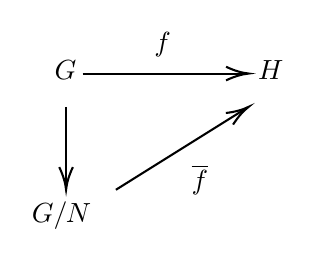
\begin{tikzpicture}[x=0.75pt,y=0.75pt,yscale=-1,xscale=1]
%uncomment if require: \path (0,476); %set diagram left start at 0, and has height of 476

%Straight Lines [id:da7538581077545223] 
\draw    (160,184) -- (238,184) ;
\draw [shift={(240,184)}, rotate = 180] [color={rgb, 255:red, 0; green, 0; blue, 0 }  ][line width=0.75]    (10.93,-3.29) .. controls (6.95,-1.4) and (3.31,-0.3) .. (0,0) .. controls (3.31,0.3) and (6.95,1.4) .. (10.93,3.29)   ;
%Straight Lines [id:da10873715429294717] 
\draw    (152,200) -- (152,238) ;
\draw [shift={(152,240)}, rotate = 270] [color={rgb, 255:red, 0; green, 0; blue, 0 }  ][line width=0.75]    (10.93,-3.29) .. controls (6.95,-1.4) and (3.31,-0.3) .. (0,0) .. controls (3.31,0.3) and (6.95,1.4) .. (10.93,3.29)   ;
%Straight Lines [id:da2888844088977629] 
\draw    (176,240) -- (238.3,201.06) ;
\draw [shift={(240,200)}, rotate = 147.99] [color={rgb, 255:red, 0; green, 0; blue, 0 }  ][line width=0.75]    (10.93,-3.29) .. controls (6.95,-1.4) and (3.31,-0.3) .. (0,0) .. controls (3.31,0.3) and (6.95,1.4) .. (10.93,3.29)   ;

% Text Node
\draw (145,176.4) node [anchor=north west][inner sep=0.75pt]    {$G$};
% Text Node
\draw (243,176.4) node [anchor=north west][inner sep=0.75pt]    {$H$};
% Text Node
\draw (134,244.4) node [anchor=north west][inner sep=0.75pt]    {$G/N$};
% Text Node
\draw (193,162.4) node [anchor=north west][inner sep=0.75pt]    {$f$};
% Text Node
\draw (211,226.4) node [anchor=north west][inner sep=0.75pt]    {$\overline{f}$};
\end{tikzpicture}
\end{center}
is commutative.
\begin{proof}
We first proof that $\overline{f}$ is well-defined. For any $b\in aN$, there exists $n\in N$ such that $b=an$. Now $f(b)=f(an)=f(a)f(n)=f(a)$ since $N\subset\mathrm{Ker}f$. Hence $\overline{f}$ has same effect on elements in $aN$. Observed that 
$$
\overline{f}\left( abN \right) =f\left( ab \right) =f\left( a \right) f\left( b \right) =\overline{f}\left( aN \right) \overline{f}\left( bN \right) ,
$$
hence $\overline{f}$ is a homomorphism. It is trivial by definition of $\overline{f}$ that $\mathrm{Im}\overline{f}=\mathrm{Im}f$. Now we proof that $\mathrm{Ker}\overline{f}=(\mathrm{Ker}f)/N$. Let $xN\in\mathrm{Ker}\overline{f}$, then $\overline{f}(xN)=f(x)=e$, hence $x\in\mathrm{Ker}f$ and therefore $xN\in(\mathrm{Ker}f/N)$. Conversely, if $yN\in(\mathrm{Ker}f)/N$, then $y\in\mathrm{Ker}f$ and hence $\overline{f}(yN)=f(y)=e$, which implies $yN\in\mathrm{Ker}\overline{f}$ and then $\mathrm{Ker}\overline{f}=(\mathrm{Ker}f)/N$. Now if $f$ is an epimorphism, then so is $\overline{f}$. If $N=\mathrm{Ker}f$, then $\mathrm{Ker}\overline{f}=\mathrm{Ker}f/\mathrm{Ker}f=\left<e\right>$. Therefore by theorem 2.9 we know that $\overline{f}$ is an isomorphism.
\end{proof}
\begin{corollary}(First Isomorphism Theorem)
If $f:G\to H$ is a homomorphism of groups, then $f$ induces an isomorphism $G/\mathrm{Ker}f\cong\mathrm{Im}f$.
\end{corollary}
This is an immediate corollary of theorem 2.35 for $G\to\mathrm{Im}f$ is epimorphic. We skip the proof.
\begin{corollary}
If $f:G\to H$ is a homomorphism of groups, $N\lhd G,M\lhd H$, and $f(N)<M$, then $f$ induces a homomorphism $\overline{f}:G/N\to H/M$, given by $aN\mapsto f(a)M$. $\overline{f}$ is an isomorphism if and only if $\mathrm{Im}f\vee M=H$ and $f^{-1}(M)\subset N$. In particular if $f$ is an epimorphism such that $f(N)=M$ and $\mathrm{Ker}f\subset N$, then $\overline{f}$ is an isomorphism.
\end{corollary}
\begin{proof}
We consider the composition 
$$
G\overset{f}{\longrightarrow}H\overset{\pi}{\longrightarrow}H/M,
$$
here $\pi f:G\to H/M$. Then by theorem 2.35 we know that $\pi f$ induces a homomorphism $\overline{f}:G/N\to H/M$ given by $aN\mapsto f(a)M$. By theorem 2.35 we know that $\overline{f}$ is an isomorphism if and only if $\pi f$ is an epimorphism and $\mathrm{Ker}\pi f=N$, which is equivalent to the condition $\mathrm{Im}f\vee M=H$ and $f^{-1}(M)\subset N$.
\end{proof}
This corollary can also be rephrased as the commutative diagram as follows:
\begin{center}
\tikzset{every picture/.style={line width=0.75pt}} %set default line width to 0.75pt        

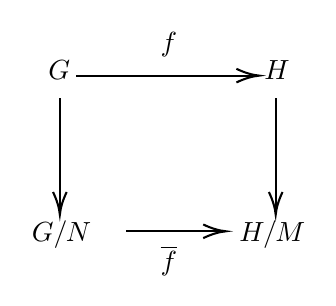
\begin{tikzpicture}[x=0.75pt,y=0.75pt,yscale=-1,xscale=1]
%uncomment if require: \path (0,476); %set diagram left start at 0, and has height of 476

%Straight Lines [id:da1481227158581686] 
\draw    (240,157) -- (326,157) ;
\draw [shift={(328,157)}, rotate = 180] [color={rgb, 255:red, 0; green, 0; blue, 0 }  ][line width=0.75]    (10.93,-3.29) .. controls (6.95,-1.4) and (3.31,-0.3) .. (0,0) .. controls (3.31,0.3) and (6.95,1.4) .. (10.93,3.29)   ;
%Straight Lines [id:da13347059157002916] 
\draw    (232,168) -- (232,222) ;
\draw [shift={(232,224)}, rotate = 270] [color={rgb, 255:red, 0; green, 0; blue, 0 }  ][line width=0.75]    (10.93,-3.29) .. controls (6.95,-1.4) and (3.31,-0.3) .. (0,0) .. controls (3.31,0.3) and (6.95,1.4) .. (10.93,3.29)   ;
%Straight Lines [id:da6724755868913452] 
\draw    (336,168) -- (336,222) ;
\draw [shift={(336,224)}, rotate = 270] [color={rgb, 255:red, 0; green, 0; blue, 0 }  ][line width=0.75]    (10.93,-3.29) .. controls (6.95,-1.4) and (3.31,-0.3) .. (0,0) .. controls (3.31,0.3) and (6.95,1.4) .. (10.93,3.29)   ;
%Straight Lines [id:da16316142037972892] 
\draw    (264,232) -- (310,232) ;
\draw [shift={(312,232)}, rotate = 180] [color={rgb, 255:red, 0; green, 0; blue, 0 }  ][line width=0.75]    (10.93,-3.29) .. controls (6.95,-1.4) and (3.31,-0.3) .. (0,0) .. controls (3.31,0.3) and (6.95,1.4) .. (10.93,3.29)   ;

% Text Node
\draw (225,148.4) node [anchor=north west][inner sep=0.75pt]    {$G$};
% Text Node
\draw (329,148.4) node [anchor=north west][inner sep=0.75pt]    {$H$};
% Text Node
\draw (217,225.4) node [anchor=north west][inner sep=0.75pt]    {$G/N$};
% Text Node
\draw (317,225.4) node [anchor=north west][inner sep=0.75pt]    {$H/M$};
% Text Node
\draw (279,134.4) node [anchor=north west][inner sep=0.75pt]    {$f$};
% Text Node
\draw (279,237.4) node [anchor=north west][inner sep=0.75pt]    {$\overline{f}$};


\end{tikzpicture}
\end{center}
\begin{corollary}(Second Isomorphism Theorem)
If $K$ and $N$ are subgroups of a group $G$, with $N$ normal in $G$, then $K/(N\cap K)\cong NK/N$.
\end{corollary}
\begin{proof}
Consider the composition 
$$
K\overset{\subset}{\longrightarrow}NK\overset{\pi}{\longrightarrow}NK/N
$$
$f$, which is a homomorphism with kernel $H\cap K$. Hence by the first Isomorphism Theorem we know that $K/(H\cap K)\cong\mathrm{Im}f$. Every element in $NK/N$ has a form of $nkN=kn^\prime N=kN$, hence $f$ is an epimorphism and $\mathrm{Im}f=KN/N$, which finished our proof.
\begin{center}
\tikzset{every picture/.style={line width=0.75pt}} %set default line width to 0.75pt        

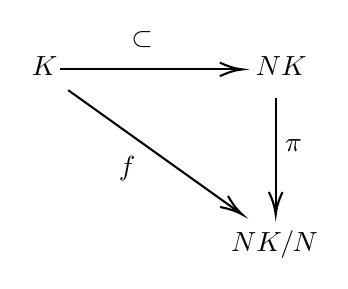
\begin{tikzpicture}[x=0.75pt,y=0.75pt,yscale=-1,xscale=1]
%uncomment if require: \path (0,476); %set diagram left start at 0, and has height of 476

%Straight Lines [id:da6768105974377752] 
\draw    (264,146) -- (350,146) ;
\draw [shift={(352,146)}, rotate = 180] [color={rgb, 255:red, 0; green, 0; blue, 0 }  ][line width=0.75]    (10.93,-3.29) .. controls (6.95,-1.4) and (3.31,-0.3) .. (0,0) .. controls (3.31,0.3) and (6.95,1.4) .. (10.93,3.29)   ;
%Straight Lines [id:da9794328893642172] 
\draw    (368,160) -- (368,214) ;
\draw [shift={(368,216)}, rotate = 270] [color={rgb, 255:red, 0; green, 0; blue, 0 }  ][line width=0.75]    (10.93,-3.29) .. controls (6.95,-1.4) and (3.31,-0.3) .. (0,0) .. controls (3.31,0.3) and (6.95,1.4) .. (10.93,3.29)   ;
%Straight Lines [id:da5963291247279754] 
\draw    (268,156) -- (350.37,214.84) ;
\draw [shift={(352,216)}, rotate = 215.54] [color={rgb, 255:red, 0; green, 0; blue, 0 }  ][line width=0.75]    (10.93,-3.29) .. controls (6.95,-1.4) and (3.31,-0.3) .. (0,0) .. controls (3.31,0.3) and (6.95,1.4) .. (10.93,3.29)   ;

% Text Node
\draw (249,138.4) node [anchor=north west][inner sep=0.75pt]    {$K$};
% Text Node
\draw (357,138.4) node [anchor=north west][inner sep=0.75pt]    {$NK$};
% Text Node
\draw (345,222.4) node [anchor=north west][inner sep=0.75pt]    {$NK/N$};
% Text Node
\draw (297,126.4) node [anchor=north west][inner sep=0.75pt]    {$\subset $};
% Text Node
\draw (371,178.4) node [anchor=north west][inner sep=0.75pt]    {$\pi $};
% Text Node
\draw (291,186.4) node [anchor=north west][inner sep=0.75pt]    {$f$};
\end{tikzpicture}
\end{center}
\end{proof}
\begin{corollary}(Third Isomorphism Theorem)
If $H$ and $K$ are normal subgroups of a group $G$ such that $K<H$, then $H/K$ is a normal subgroup of $G/K$ and $(G/K)(H/K)\cong G/H$.
\end{corollary}
\begin{proof}
Define $f:G/K\rightarrow G/H$ by $aK\mapsto aH$. From $K<H$ we know that $f$ is an epimorphism. Consider the kernel of $f$, we have 
$$
\mathrm{Ker}f=\left\{ aK:a\in H \right\} =H/K
$$
since $f(aK)\in H$ if and only if $a\in H$. Therefore $\mathrm{Ker}f=H/K\lhd G/K$ and hence 
$$
\mathrm{Im}f=G/H\cong \left( G/K \right) /\left( \mathrm{Ker}f \right) =\left( G/K \right) /\left( H/K \right) .
$$
\begin{center}
\tikzset{every picture/.style={line width=0.75pt}} %set default line width to 0.75pt        

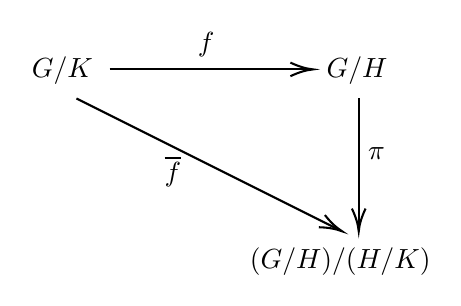
\begin{tikzpicture}[x=0.75pt,y=0.75pt,yscale=-1,xscale=1]
%uncomment if require: \path (0,476); %set diagram left start at 0, and has height of 476

%Straight Lines [id:da6750362936107648] 
\draw    (248,162) -- (344,162) ;
\draw [shift={(346,162)}, rotate = 180] [color={rgb, 255:red, 0; green, 0; blue, 0 }  ][line width=0.75]    (10.93,-3.29) .. controls (6.95,-1.4) and (3.31,-0.3) .. (0,0) .. controls (3.31,0.3) and (6.95,1.4) .. (10.93,3.29)   ;
%Straight Lines [id:da9589750420240954] 
\draw    (368,176) -- (368,238) ;
\draw [shift={(368,240)}, rotate = 270] [color={rgb, 255:red, 0; green, 0; blue, 0 }  ][line width=0.75]    (10.93,-3.29) .. controls (6.95,-1.4) and (3.31,-0.3) .. (0,0) .. controls (3.31,0.3) and (6.95,1.4) .. (10.93,3.29)   ;
%Straight Lines [id:da8916432325404353] 
\draw    (232,176) -- (358.21,239.11) ;
\draw [shift={(360,240)}, rotate = 206.57] [color={rgb, 255:red, 0; green, 0; blue, 0 }  ][line width=0.75]    (10.93,-3.29) .. controls (6.95,-1.4) and (3.31,-0.3) .. (0,0) .. controls (3.31,0.3) and (6.95,1.4) .. (10.93,3.29)   ;

% Text Node
\draw (209,154.4) node [anchor=north west][inner sep=0.75pt]    {$G/K$};
% Text Node
\draw (351,154.4) node [anchor=north west][inner sep=0.75pt]    {$G/H$};
% Text Node
\draw (314,246.4) node [anchor=north west][inner sep=0.75pt]    {$( G/H) /( H/K)$};
% Text Node
\draw (289,142.4) node [anchor=north west][inner sep=0.75pt]    {$f$};
% Text Node
\draw (371,198.4) node [anchor=north west][inner sep=0.75pt]    {$\pi $};
% Text Node
\draw (273,202.4) node [anchor=north west][inner sep=0.75pt]    {$\overline{f}$};


\end{tikzpicture}
\end{center}
\end{proof}
\begin{theorem}
If $f:G\to H$ is an isomorphism of groups, then the assignment $K\mapsto f(K)$ defines a one-to-one correspondence between the set $S_f(G)$ of all subgroups $K$ of $G$ which contain $\mathrm{Ker}f$ and the set $S(H)$ of all subgroups of $H$. Under this correspondence normal subgroups correspond to normal subgroups.
\end{theorem}
\begin{proof}
Denote $\varphi:S_f(G)\to S(H)$ given by $K\mapsto f(K)$. We first proof that $\varphi$ is bijective. By exercise 2.20 we know that for all $J\in S(H)$, $f^{-1}(J)$ is a subgroup of $G$. Since $J<H$, we have $\mathrm{Ker}f<f^{-1}(J)$ and hence $f(f^{-1}(J))=J$. That is, for all $J\in S(H)$, there exists $f^{-1}(J)\in S_f(G)$ such that $f(f^{-1}(J))=J$, hence $\varphi$ is surjective. By an exercise of this section(we shall admit this to be true here) we know that $f^{-1}(f(J))=J$ if and only if $\mathrm{Ker}f<J$, which is
$$
f\left( K \right) =f\left( J \right) \Rightarrow K=f^{-1}\left( f\left( K \right) \right) =f^{-1}\left( f\left( J \right) \right) =J\Rightarrow K=J,
$$
hence $\varphi$ is injective. For the last statement, we proof that $K\lhd G$ implies $f(K)\lhd H$, which is easy to verify by definition of a normal group. Similarly we have $J\lhd H$ implies $f^{-1}(J)\lhd G$.
\end{proof}
\begin{corollary}
If $G$ is a group and $N$ is a normal subgroup of $G$, then every subgroup of $G/N$ has a form of $K/N$, where $K$ is a subgroup of $G$ that contains $N$. Furthermore, $K/N$ is normal in $G/N$ if and only if $K$ is normal in $G$.
\end{corollary}
\begin{proof}
Apply theorem 2.40 to the canonical mapping $\pi:G\to G/N$. It is familiar to us that $\mathrm{Ker}\pi=N$, hence by theorem 2.40, any subgroup $K$ satisfies $N<K<G$ corresponds with a subgroup $K/N$ satisfies $K/N<G/N$. Since the correspondence is one-to-one, we know all subgroups of $G/N$ has such a form.Also if $K/N$ is a normal subgroup of $G/N$, then $K\lhd G$.The converse statement is also true since the correspondence is one-to-one.
\end{proof}
\begin{center}
\begin{large}
    \textbf{Exercises for 2.5}
\end{large}
\end{center}
\begin{problem}\em
If $N$ is a subgroup of index $2$ in a group $G$, then $N$ is normal in $G$.
\end{problem}
\begin{proof}
We consider all cosets of $N$ in $G$. Clearly $N$ itself is a coset of $N$. Since $[G:N]=2$, then another coset is the complement of $N$ since cosets completely separated $G$. Observed the discussion above does not involve the concept of a left coset or right coset, hence they are totally symmetric. By definition of normal group we have $N\lhd G$.
\end{proof}
\begin{problem}\em
If $\{N_i:i\in I\}$ is a family of normal subgroups of $G$, then $\bigcap_{i\in I}N_i$ is a normal subgroup of $G$.
\end{problem}
\begin{proof}
We proof by definition. Take $n\in\bigcap_{i\in I}N_i$, then for any $i\in I$ and $a\in G$ we have $ana^{-1}\in N_i$ since $N_i\lhd G$. Since this is generally true for all $i\in I$, we know that $ana^{-1}\in\bigcap_{i\in I}N_i$, which implies $a\left(\bigcap_{i\in I}N_i\right)a^{-1}\subset\bigcap_{i\in I}N_i$ and hence $\left(\bigcap_{i\in I}N_i\right)\lhd G$.
\end{proof}
\begin{problem}\em
Let $N$ be a subgroup of $G$. $N$ is normal in $G$ if and only if (right) congruence modulo $N$ is a congruence relation on $G$.
\end{problem}
\begin{proof}
Suppose $N$ is normal in $G$. If $a_1\equiv b_1(\mathrm{mod}N)$ and $a_2\equiv b_2(\mathrm{mod}N)$, then $a_1b_1^{-1}\in N,a_2b_2^{-1}\in N$. It suffices to show that $a_1a_2b_2^{-1}b_1^{-1}\in G$, which can be obtained by the same trick used in Theorem 2.33. Conversely, by definition of a congruence relation and $n\equiv e(\mathrm{mod}N)$, $a\equiv a(\mathrm{mod}N)$, here $n\in N$ and $a\in G$ are arbitrarily chosen, we have $an\equiv a(\mathrm{mod}N)$ and hence $ana^{-1}\in N$. Therefore $aNa^{-1}\subset N$ for all $a\in G$ and hence $N\lhd G$.
\end{proof}
\begin{problem}\em
Let $\sim$ be an equivalence relation on a group $G$ and let $N=\{a\in G:a\sim e\}$. Then $\sim$ is a congruence relation on $G$ if and only if $N$ is a normal subgroup of $G$ and $\sim$ is congruence modulo $N$.
\end{problem}
\begin{proof}
Let $\sim$ be a congruence relation on $G$. Hence for all $n\in N$ and $a\in G$ we have $ana^{-1}\sim e$ by the same method used in exercise 2.56, hence $ana^{-1}\in N$. Therefore $aNa^{-1}\in N$ and $N\lhd G$. What's more, if $a\sim b$, then $ab^{-1}\sim e$, which is $ab^{-1}\in N$, hence $\sim$ is congruence modulo $N$. The converse condition is trivial.
\end{proof}
\begin{problem}\em
Let $N<S_4$ consist of all those permutations $\sigma$ such that $\sigma(4)=4$. Is $N$ normal in $S_4$?
\end{problem}
\begin{proof}
No. Take 
$$
\sigma =\left( \begin{matrix}
	1&		2&		3&		4\\
	2&		3&		1&		4\\
\end{matrix} \right) \in N,\tau =\left( \begin{matrix}
	1&		2&		3&		4\\
	2&		3&		4&		1\\
\end{matrix} \right) \in S_4,
$$
then $\tau \sigma \tau ^{-1}\left( 4 \right) =2\ne 4$, hence $\tau\sigma\tau^{-1}\notin N$.
\end{proof}
\begin{problem}\em
Let $H<G$. Then the set $aHa^{-1}$ is a subgroup for each $a\in G$, and $H\cong aHa^{-1}$.
\end{problem}
\begin{proof}
First since $H$ is a subgroup then $e\in H$, we know that $e=aa^{-1}=aea^{-1}\in aHa^{-1}$. Then if $aha^{-1}\in aHa^{-1}$, since $G$ and $H$ are all groups, we have $a^{-1}\in G$ and $h^{-1}\in H$, therefore $ah^{-1}a^{-1}\in aHa^{-1}$. Hence $aHa^{-1}$ is a subgroup of $G$. Now define $f:aHa^{-1}\to H$ by $aha^{-1}\mapsto h$, it is easy to verify $f$ is an isomorphism and hence $H\cong aHa^{-1}$.
\end{proof}
\begin{problem}\em
Let $G$ be a finite group and $H$ be a subgroup of $G$ ordered $n$. If $H$ is the only subgroup of $G$ of order $n$, then $H$ is normal in $G$.
\end{problem}
\begin{proof}
Let $a\in G$. Then by exercise 2.59 we know that $H\cong aHa^{-1}$. Therefore $aHa^{-1}$ is also a subgroup of $G$ with order $n$. However there is only one such subgroup, we have $H=aHa^{-1}$ and hence $H\lhd G$.
\end{proof}
\begin{problem}\em
All subgroups of the quaternion group are normal.
\end{problem}
\begin{proof}
We denote 
$$
I=\left( \begin{matrix}
	0&		\mathrm{i}\\
	\mathrm{i}&		0\\
\end{matrix} \right) ,J=\left( \begin{matrix}
	0&		1\\
	1&		0\\
\end{matrix} \right) ,K=\left( \begin{matrix}
	\mathrm{i}&		0\\
	0&		-\mathrm{i}\\
\end{matrix} \right) ,L=-I.
$$
Then subgroups of $Q_8$ are $0,\left< L \right> ,\left< I \right> ,\left< J \right> ,\left< K \right> ,Q_8$. Both $0$ and $Q_8$ are trivial normal subgroups. Subgroups generated by $I,J$ and $K$ have an order $2$. Finally $L$ is the intersection of normal groups. Hence by exercise 2.54 and exercise 2.55 we finished our proof.
\end{proof}
\begin{note}\em
Notice that $Q_8$ is non-abelian. This exercise gives an example that a group with all its subgroups normal may not be abelian.
\end{note}
\begin{problem}\em
(a) If $G$ is a group, then the center of $G$ is normal subgroup of $G$.\par
(b) The center of $S_n$ is the identity subgroup for all $n>2$.
\end{problem}
\begin{proof}
(a) We denote the center of $G$ as $C$. For all $x\in C$ we have $ax=xa$, where $a\in G$ is arbitrarily chosen. Hence $aC=Ca$ holds for all $a$ and therefore $C\lhd G$.\par
(b) We denote the center of $S_n$ as $Z(S_n)$. If there exists such an element $\sigma$ that $\sigma\ne(1)$, WLOG we suppose $\sigma(1)=2$, then for $\tau=(23)$, we observed that $\sigma\tau(1)=2$ and $\tau\sigma=3$, which contradicts to the definition of the center of a group.
\end{proof}
\begin{problem}\em
Find subgroups $H$ and $K$ of $D_4^*$ such that $H\lhd K$ and $K\lhd D_4^*$, but $H$ is not normal in $D_4^*$.
\end{problem}
\begin{proof}
Consider the subgroup $H$ generated by $T_x$, which is a subgroup of the group $K$ generated by $R^2$ and $T_x$ with index $2$. Therefore by exercise 2.54 we know that $H$ is normal in $K$. Also $K$ is a subgroup of index $2$ in $D_4^*$, hence $K$ is normal in $D_4^*$. However, we may check that $H$ is not normal in $D_4^*$.
\end{proof}
\begin{note}\em
This exercise provided an example that normality may not be transitive.
\end{note}
\begin{problem}\em
If $H$ is a cyclic subgroup of a group $G$ and $H$ is normal in $G$, then every subgroup of $H$ is normal in $G$.
\end{problem}
\begin{proof}
Let $H=\left<a\right>$. Then if $K$ is a subgroup of $H$, take $k\in K$, it has the form $k=a^j$, here $j\in\mathbb{Z}$. Since $H$ is normal in $G$, then for all $g\in G$ we have $ga^jg^{-1}=(gag^{-1})^k=a^{mk}\in K$, hence $gKg^{-1}\subset K$ and therefore $K$ is normal in $G$.
\end{proof}
\begin{problem}\em
If $H$ is a normal subgroup of a group $G$ such that $H$ and $G/H$ are finitely generated, then so is $G$.
\end{problem}
\begin{proof}
Suppose $H$ is generated by a finite set $X$ and $G/H$ is generated by a finite group $Y$. It suffices to show that $G$ is generated by $X\cup Y$. Now observed that 
$$
G=\bigcup_{a\in G}{aH}=\bigcup_{x_i\in X}{\left( \prod_i{x_{i}^{r_i}H} \right)}=\bigcup_{x_i\in X}{\left( \prod_i{x_{i}^{r_i}\left( \bigcup_{y_j\in Y}{\prod_j{y_{j}^{s_j}}} \right)} \right)}=\bigcup_X{\bigcup_Y{\left( \prod_i{\prod_j{x_{i}^{r_i}y_{j}^{s_j}}} \right)}},
$$
hence $G$ is generated by $X\cup Y$ and we finished our proof.
\end{proof}
\begin{problem}\em
Let $H\lhd G,K\lhd G$. Show that $H\vee K$ is normal in $G$.
\end{problem}
\begin{proof}
Since $H$ and $K$ are normal in $G$, then $H\vee K=HK$ by Theorem 2.32. Hence for all $x\in H\vee K$, we may set $x=hk$. Now since $H$ and $K$ are all normal in $G$, for all $g\in G$ we have $gxg^{-1}=ghgg^{-1}kg\in HK$, hence $gHKg^{-1}\subset HK$ and therefore $H\vee K=HK$ is normal in $G$.
\end{proof}
\begin{problem}\em
If $N_1\lhd G_1,N_2\lhd G_2$ then $(N_1\times N_2)\lhd(G_1\times G_2)$ and $(G_1\times G_2)/(N_1\times N_2)\cong(G_1/N_1)\times(G_2/N_2)$.
\end{problem}
\begin{proof}
Let $(n_1,n_2)\in N_1\times N_2$. Then for $(g_1,g_2)\in G_1\times G_2$, then since $N_1\lhd G_1,N_2\lhd G_2$ we know that 
$$
\left( g_1,g_2 \right) \left( n_1,n_2 \right) \left( g_1,g_2 \right) ^{-1}=\left( g_1n_1g_{1}^{-1},g_2n_2g_{2}^{-1} \right) \in N_1\times N_2,
$$
hence $\left( g_1,g_2 \right) \left( N_1\times N_2 \right) \left( g_1,g_2 \right) ^{-1}\subset N_1\times N_2$, whence $N_1\times N_2$ is normal in $G_1\times G_2$. Now define $f:(G_1\times G_2)/(N_1\times N_2)\to(G_1/N_1)\times(G_2/N_2)$ by $\left( g_1,g_2 \right) \left( N_1\times N_2 \right) \mapsto \left( g_1N_1,g_2N_2 \right) $, it is easy to verify that $f$ is an isomorphism.
\end{proof}
\begin{problem}\em
Let $N\lhd G$ and $K\lhd G$. If $N\cap K=\left<e\right>$ and $N\vee K=G$, then $G/N\cong K$.
\end{problem}
\begin{proof}
We proof by the Second Homomorphism Theorem, by which we know that $HN/N\cong K/(H\cap K)$. However, since $N$ and $K$ are normal in $G$, we know by theorem 2.32 that $HN=H\vee N=G$. Also observed that $N\cap K=\left<e\right>$, hence $HN/N=G/N\cong K/(N\cap K)=K$.
\end{proof}
\begin{problem}\em
If $f:G\to H$ is a homomorphism, $H$ is abelian and $N$ is a subgroup of $G$ containing $\mathrm{Ker}f$, then $N$ is normal in $G$.
\end{problem}
\begin{proof}
We proof by the First Homomorphism Theorem, by which we know that $G/\mathrm{Ker}f\cong\mathrm{Im}f$. It suffices to show that $N/\mathrm{Ker}f\lhd G/\mathrm{Ker}f$ by theorem 2.40. Since $G/\mathrm{Ker}f\cong\mathrm{Im}f$, we only need to proof $N/\mathrm{Ker}f\lhd\mathrm{Im}f$. Since $H$ is abelian and $\mathrm{Im}f$ is a subgroup of $H$, clearly $\mathrm{Im}f$ is also abelian. Then $N/\mathrm{Ker}f\lhd\mathrm{Im}f$ follows immediately since all subgroups of an abelian group are normal, since $aha^{-1}=aa^{-1}h=h\in H$ for all $h\in N/\mathrm{Ker}f$ and $a\in\mathrm{Im}f$.
\end{proof}
\begin{problem}\em
(a) Consider the subgroups $\left<6\right>$ and $\left<30\right>$ of $\mathbb{Z}$ and show that $\left<6\right>/\left<30\right>\cong\mathbb{Z}_5$.\par
(b) For any $k,m>0$, $\left<k\right>/\left<km\right>\cong\mathbb{Z}_m$. In particular, $\mathbb{Z}/\left<m\right>\cong\mathbb{Z}_m$.
\end{problem}
\begin{proof}
(a) Observed that 
$$\left<6\right>/\left<30\right>=\{\left<30\right>,6+\left<30\right>,12+\left<30\right>,18+\left<30\right>,24+\left<30\right>\},$$
we may define $f:\left<6\right>/\left<30\right>\to\mathbb{Z}_5$ by $6m+\left<30\right>\mapsto\overline{m}$, which is easy to verify to be an isomorphism.\par
(b) Observed that 
$$
\left< m \right> /\left< km \right> =\left\{ \left< km \right> ,m+\left< km \right> ,2m+\left< km \right> ,\cdots ,\left( k-1 \right) m+\left< km \right> \right\} ,
$$
by same method used for (a) we may define an isomorphism from $\left<m\right>/\left<km\right>$ to $\mathbb{Z}_m$, which shows that $\left<k\right>/\left<km\right>\cong\mathbb{Z}_m$.
\end{proof}
\begin{problem}\em
If $f:G\to H$ is a homomorphism with kernel $N$ and $K<G$, then prove that $f^{-1}(f(K))=KN$.
\end{problem}
\begin{proof}
First observed 
$$
\begin{aligned}
f^{-1}\left( f\left( K \right) \right) &=\left\{ x\in G:f\left( k \right) =f\left( x \right) \,\,\mathrm{for} \mathrm{some} k\in K \right\} 
\\
&=\left\{ x\in G:kx^{-1}\in N,\in K \right\} =\left\{ x\in G:x\in kN,k\in K \right\} \subset KN,
\end{aligned}
$$
hence $f^{-1}f(K)\subset KN$. Conversely, for $x\in KN$, let $x=kn$, then 
$$
f^{-1}\left( f\left( kn \right) \right) =f^{-1}\left( f\left( k \right) f\left( n \right) \right) =f^{-1}\left( f\left( k \right) \right) \in f^{-1}\left( f\left( K \right) \right) ,
$$
therefore $f^{-1}(f(K))\supset KN$, hence $f^{-1}(f(K))=KN$.
\end{proof}
\begin{note}\em
By this exercise we know that $f^{-1}(f(K))=K$ if and only if $N<K$, which is used in the proof of theorem 2.40.
\end{note}
\begin{problem}\em
If $N\lhd G$, $[G:N]$ finite, $H<G$, $G$ finite, and $[G:N]$ and $|H|$ are relatively prime, then $H<N$.
\end{problem}
\begin{proof}
Let $G=N\cup a_1N\cup \cdots \cup a_nN$. It suffices to show $N\subset H$. Let $a\in H$, then $a=a_in,n\in N,i\in\{1,2,\cdots,n\}$. Since $N$ is normal in $G$, we have $(a_in)^{|H|}=e\Rightarrow a_i^{|H|}n^{|H|}=e$. However $a_i^{[G:N]}=e$ and $[G:N]$ and $|H|$ are relatively prime, hence $a_i\in N$, which implies $a\in N$ and we finished our proof.
\end{proof}
\begin{problem}\em
Let $H\ne\mathbb{Z}(p^\infty)$ be a subgroup of $\mathbb{Z}(p^\infty)$, prove that $\mathbb{Z}(p^\infty)/H\cong\mathbb{Z}(p^{\infty})$.
\end{problem}
\begin{proof}
First $H$ must be a cyclic subgroup with all its elements have a finite order by exercise 2.36. Let $H_i=\left<\overline{1/p^i}\right>$. Now we have the canonical projection homomorphisms $\pi_i:\mathbb{Z}(p^\infty)\to\mathbb{Z}(p^\infty)/H_i$. Notice the image contains elements $x_n=\overline{1/p^{n+i}}+H_i$, therefore
$$
px_{n+1}=pf\left( \overline{1/p^{\left( n+1 \right) +i}} \right) =f\left( \overline{p/p^{\left( n+1 \right) +i}} \right) =f\left( \overline{1/p^{n+i}} \right) =x_n,
$$
Also $i$ is finite, so $x_n$ exists for any $n\in\mathbb{Z}_+$. Therefore by exercise 2.36 we know that $\mathbb{Z}(p^\infty)/H\cong\mathbb{Z}(p^{\infty})$.
\end{proof}
\subsection{Symmetric, Alternating, and Dihedral Groups}
In this section we shall study in some detail the symmetric group $S_n$ and its subgroups. By definition $S_n$ is a bijection $I_n\to I_n$, where $I_n=\{1,2,\cdots,n\}$. We first introduce another notation of a permutation:
\begin{definition}
Let $i_1,i_2,\cdots,i_r$ be distinct elements of $I_n$, here $r\le n$. Then $(i_1i_2\cdots i_n)$ denotes a permutation that maps $i_1\mapsto i_2,i_2\mapsto i_3,\cdots,i_r\mapsto i_1$, and maps every other elements in $I_n$ onto itself. $(i_1i_2\cdots i_n)$ is called a \textbf{cycle with length $r$} or an \textbf{$r$-cycle}. In particular, a $2$-cycle is called a \textbf{transposition}.
\end{definition}
Here are some examples.
\begin{example}\em
A permutation $
\sigma =\left( \begin{matrix}
	1&		2&		3&		4\\
	2&		3&		4&		1\\
\end{matrix} \right) 
$ is a $4$-cycle denote as $(1234)$ or $(2341)$ or $(3412)$ or $(4123)$.
\end{example}
As we can see a cycle may be written in many different ways. However, one may eliminate ambiguities by context.\par
There is one condition that some cycles are commute.
\begin{definition}
The permutations $\sigma_1,\sigma_2,\cdots,\sigma_r$ of $S_n$ is said to be \textbf{disjoint} provided for each $1\le i\le r$, and every $k\in I_n,\sigma_i(k)\ne k$ implies $\sigma_j(k)=k$ for all $j\ne i$.
\end{definition}
In other words, $\sigma_1,\sigma_2,\cdots,\sigma_r$ are said to be disjoint if and only if no element of $I_n$ is moved by more than one of $\sigma_i,1\le i\le r$.
\begin{example}\em
In $S_4$, the transposition $(13)$ and $(24)$ are disjoint. It is easy to verify that disjoint cycles are commute since every element is only moved once.
\end{example}
We have the important theorem as follows:
\begin{theorem}
Every non-identity permutation in $S_n$ is uniquely a product of disjoint cycles, each of which has length at least $2$.
\end{theorem}
\begin{proof}
Let $\sigma$ be a non-trivial permutation in $S_n$. We first proof that there exists some disjoint cycles of length at least $2$, such that $\sigma$ is the product of them. We begin by define a relation on $I_n$: $a\sim b$ for $a,b\in I_n$ if and only if $b=\sigma^m(a)$ for some $m\in\mathbb{Z}$. Now we proof $\sim$ is an equivalence relation:\par
(i) $a\sim a$: This is trivial.\par
(ii) $a\sim b\Rightarrow b\sim a$: By $a\sim b$ we know that there exists $m\in\mathbb{Z}$ such that $b=\sigma^m(a)$, hence $a=\sigma^{-m}(b)$ and therefore $a\sim b$.\par
(iii) $a\sim b,b\sim c\Rightarrow a\sim c$: By $a\sim b$ and $b\sim c$ we know that there exists $m,n\in\mathbb{Z}$ such that $b=\sigma^m(a)$ and $c=\sigma^n(b)$, hence $c=\sigma^{m+n}(a)$, therefore $a\sim c$.\par
Now $\sim$ is an equivalence relation and therefore it induces equivalence classes $\{B_i\}$, where $B_i=\{x:x\sim x_i\}=\{\sigma^m(x_i):m\in\mathbb{Z}\}$, here $x_i$ is a select element in $I_n$. By properties of equivalent classes we know $B_i$ are disjoint. We call $B_i=\{\sigma^m(x_i):m\in\mathbb{Z}\}$ the \textbf{orbit of $x_i$ generated by $\sigma$}. Now we define $
\sigma _i\left( x \right) =\begin{cases}
	\sigma \left( x \right) ,x\in B_i,\\
	x,x\notin B_i,\\
\end{cases}
$ it is easy to verify $\sigma=\sigma_1\sigma_2\cdots\sigma_s$, here we assume the index class of $\{B_i\}$ is $1,2,\cdots,s$, that is, $1\le i\le s$. Now it suffices to show that for any $x\in I_n$ there exists $d\in\mathbb{Z}_+$ such that $\sigma^d(x)=x$, since $\sigma_j$ are disjoint and hence $\sigma(x)=\sigma_i(x)$ for some $i\in I_s$. First, we know that there exists a least $d$ such that $\sigma^d(x)=\sigma^j(x)$ for some $0\le j<d$, since $S_n$ is obviously finite. Therefore $\sigma^{d-j}(x)=x$, which forces $j=0$ and $\sigma^d(x)=x$. Now for any $m\in\mathbb{Z}$, there exists $a,b\in\mathbb{Z}$ such that $m=ad+b$, hence $\sigma^m(x)=\sigma^{ad+b}(x)=\sigma^b(x)\in B_i$ for a unique $i\in I_s$, therefore we proved that $\sigma_i$ is a cycle. Since $x\in I_n$ is arbitrarily chosen, the result is true for all $\sigma_j$.\par
Now we proof that the product of disjoint cycles are unique. If there is another presentation $\tau_1\tau_2\cdots\tau_t$, then for all $x\in I_n$, there exists unique $i$ and $j$ such that $\sigma_i(x)=\tau_j(x)$. Since $\sigma\tau_j=\tau_j\sigma$, we know that the orbit generated by $\sigma_i$ is precisely the orbit generated by $\tau_j$, and since permutations discussed here are all cycles, it suffices to show that cycles have only one non-trivial orbit. Let $(i_1i_2\cdots i_r)$ be a cycle. If $i_k\ne i_j,j=1,2,\cdots,r$, then $i_k$ generates a trivial orbit. Otherwise we have the orbit 
$$
i_k\rightarrow i_{k+1}\rightarrow \cdots \rightarrow i_r\rightarrow i_1\rightarrow \cdots \rightarrow i_{k-1},
$$
which is easy to see is equivalent for all $k\in I_r$. Hence by induction we finished our proof.
\end{proof}
\begin{corollary}
The order of a permutation $\sigma\in S_n$ is the least common multiple of the orders of its disjoint cycles.
\end{corollary}
\begin{proof}
By theorem 2.44 we know that $\sigma$ can be written as the product of some cycles $\sigma_1\sigma_2\cdots\sigma_r$. Now if $\sigma^m(x)=x$ for all $x\in I_n$, then $\sigma_j^m(x)=x$ for all $j=1,2,\cdots,r$. Therefore $m$ is multiple of the order of $\sigma_j$. Since this is true for all $j=1,2,\cdots,r$, we finished our proof.
\end{proof}
\begin{corollary}
Every permutation in $S_n$ can be written as a product of some transpositions(not necessarily disjoint).
\end{corollary}
\begin{proof}
By theorem 2.44 we know that $\sigma\in S_n$ can be written as the product of some cycles $\sigma_1\sigma_2\cdots\sigma_r$. It suffices to show that for all cycles $\sigma_j$, it can be written as product of some transpositions. This is clearly true since if the length of cycle is $2$, then it itself is a transposition, otherwise let $(i_1i_2\cdots i_r)$ be the cycle, observed that $(i_1i_2\cdots i_r)=(i_1i_r)(i_2i_r)\cdots(i_{r-1}i_r)$.
\end{proof}
\begin{definition}
A permutation $\tau\in S_n$ is said to be \textbf{even} [resp. \textbf{odd}] if $\tau$ can be written as a product of an even [resp. odd] number of transpositions.
\end{definition}
We have to check if an even [resp. odd] permutation is well-defined. That is, can a permutation be both even and odd?
\begin{theorem}
A permutation in $S_n(n\ge 2)$ is either odd or even.
\end{theorem}
\begin{proof}
Let $i_1,i_2,\cdots,i_n$ be integers $1,2,\cdots,n$ in some order. Define 
$$
\Delta \left( i_1,i_2,\cdots ,i_n \right) =\prod_{1\le j<k\le n}{\left( i_j-i_k \right)}.
$$
It is clear that $\Delta(i_1,i_2,\cdots,i_n)\ne 0$. Let $\sigma=(i_ci_d)$ be a transposition and we compute $\Delta(\sigma(i_1),\sigma(i_2),\cdots,\sigma(i_n))$:
$$
\Delta \left( \sigma \left( i_1 \right) ,\sigma \left( i_2 \right) ,\cdots ,\sigma \left( i_n \right) \right) =\prod_{1\le j<k\le n}{\left( \sigma \left( i_j \right) -\sigma \left( i_k \right) \right)}=\prod_{j<k,j,k\ne c,d}{\left( i_j-i_k \right)}\cdot \left( i_d-i_c \right) .
$$
Hence $\Delta(i_1,i_2,\cdots,i_n)=-\Delta(\sigma(i_1),\sigma(i_2),\cdots,\sigma(i_n))$. Now suppose $\sigma\in S_n$ is both even and odd, then 
$$
\Delta \left( \sigma \left( i_1 \right) ,\sigma \left( i_2 \right) ,\cdots ,\sigma \left( i_n \right) \right) =\left( -1 \right) ^s\Delta \left( i_1,i_2,\cdots ,i_n \right) =\left( -1 \right) ^t\Delta \left( i_1,i_2,\cdots ,i_n \right) ,
$$
therefore $\Delta(i_1,i_2,\cdots,i_n)=0$, a contradiction!
\end{proof}
\begin{theorem}
For each $n\ge 2$, let $A_n$ be the set of all even permutations of $S_n$. Then $A_n$ is a normal subgroup of $S_n$ of index $2$ and order $\frac{|S_n|}{2}$. Furthermore, $A_n$ is the only subgroup of $S_n$ of index $2$.
\end{theorem}
\begin{proof}
Let $C$ be the multiplicative group $\{-1,1\}$. Define a homomorphism $f:S_n\to C$ by $\sigma\mapsto\mathrm{sgn}\sigma$, where $\mathrm{sgn}\sigma$ is defined as follows:
$$
\mathrm{sgn} \sigma =\begin{cases}
	1,\sigma \,\,\mathrm{is}\, \mathrm{even},\\
	-1,\sigma \,\,\mathrm{is}\, \mathrm{odd},\\
\end{cases}
$$
Then by the First Isomorphism Theorem we have $S_n/\mathrm{Ker}f\cong\mathrm{Im}f$, where $\mathrm{Ker}f=A_n$. Since $\mathrm{Ker}f\lhd S_n$ we know that $A_n\lhd S_n$. What's more, $\mathrm{Im}f=C$ and hence $S_n/A_n\cong C$, therefore $[S_n:A_n]=2$ and $|A_n|=\frac{|S_n|}{2}$. We will proof the uniqueness in exercises.
\end{proof}
\begin{note}\em
The group $A_n$ is called the \textbf{alternating group on $n$ letters} or the \textbf{alternating group of degree $n$}.
\end{note}
\begin{definition}
A group $G$ is said to be \textbf{simple} if $G$ has no proper normal subgroups.
\end{definition}
The only abelian simple groups are $\mathbb{Z}_p$ where $p$ is prime as shown in exercise 2.42. There are many non-abelian simple groups. Now we proof that all $A_n$ except $A_4$ are simple groups.
\begin{theorem}
The alternating group $A_n$ is simple if and only if $n\ne 4$.
\end{theorem}
\begin{proof}
Let $N$ be a nontrivial normal subgroup of $A_n$. We proof $N=A_n$ by several steps.\par
(i) $N$ contains a $3$-cycle. Let $\sigma\in N$. First of all $\sigma$ must rearrange the position of at least $3$ elements in $I_n$, or otherwise $\sigma$ is a transposition, which is odd. If $\sigma$ rearrange precisely $4$ elements in $I_n$, then $\sigma=(a_1a_2)(a_3a_4)$, where $a_i(1\le i\le 4)$ are elements of $I_n$ being rearranged. Since $n\ge 5$, $\beta(a_3a_4a_5)\in A_n$, hence $\sigma_1=\beta\sigma\beta^{-1}=(a_1a_3a_4a_2\cdots)\cdots\in N$. Therefore $\sigma\sigma_1=(a_3a_4)(a_4a_5)=(a_3a_4a_5)\in N$. If $\sigma$ rearrange at least $5$ elements, then we discuss each case below separately:\par
\textbf{Case 1}: $\sigma$ contains a cycle of length more than $4$. Let $\sigma=(a_1a_2a_3a_4\cdots)\cdots$. Take $\beta=(a_2a_3a_4)\in A_n$, therefore $\sigma_1=\beta\sigma\beta^{-1}=(a_1a_3a_4a_2\cdots)\cdots\in N$. Hence there are at most $4$ elements being rearranged in $\sigma_1\sigma^{-1}$, a contradiction!\par
\textbf{Case 2}: $\sigma$ has its longest cycle of length $3$. Let $\sigma=(a_1a_2a_3)(a_4a_5\cdots)\cdots$. Since $\sigma$ rearranges at least $5$ elements in $I_n$, $\sigma$ is not a cycle of length $3$. Hence such $\sigma$ must rearrange at least $6$ elements. Take $\beta=(a_2a_3a_4)\in A_n$, then $\sigma_1=\beta\sigma\beta^{-1}=(a_1a_3a_4)(a_2a_5\cdots)\cdots\in N$, which rearrange at most $5$ elements, a contradiction!\par
\textbf{Case 3}: $\sigma$ be the product of some transpositions. Let $\sigma=(a_1a_2)(a_3a_4)\cdots$, it rearranges at least $6$ elements. Take $\beta=(a_2a_3a_4)\in A_n$, then $\sigma_1=\beta\sigma\beta^{-1}=(a_1a_3)(a_4a_2)\cdots\in N$, and $\sigma\sigma_1^{-1}$ rearranged only $4$ elements, a contradiction!\par
(ii) Let $a_1,a_2$ be distinct elements of $I_n$. Then $A_n$ is generated by the $3$-cycles $\{(a_1a_2a_k):k=3,4,\cdots\}$. Every element of $A_n$ is a product of terms of the form $(a_1a_2)(a_3a_4)$ or $(a_1a_2)(a_1a_3)$, since $(a_1a_2)(a_3a_4)=(a_1a_3a_2)(a_1a_3a_4)$ and $(a_1a_2)(a_1a_3)=(a_1a_3a_2)$, $A_n$ is generated by the set of all $3$-cycles. Any $3$-cycle is of the form 
$$(a_1a_ka_2),(a_1a_2a_k),(a_1a_ka_r),(a_2a_ka_r),(a_ka_ra_s),$$ where $a_k,a_r,a_s$ are distinct from each other and $a_1,a_2$. Since 
$$
\left( a_1a_ka_2 \right) =\left( a_1a_2a_k \right) ^2,\left( a_1a_ka_r \right) =\left( a_1a_2a_r \right) \left( a_1a_2a_k \right) ^2,
$$
$$
\left( a_2a_ka_r \right) =\left( a_1a_2a_r \right) ^2\left( a_1a_2a_k \right) ,\left( a_ka_ra_s \right) =\left( a_1a_2a_k \right) ^2\left( a_1a_2a_s \right) \left( a_1a_2a_k \right) ^2\left( a_1a_2a_k \right) ,
$$
we know that $A_n$ is generated by all $3$-cycles of the form $(a_1a_2a_k)$.\par
(iii) Now if $N$ is a nontrivial normal subgroup of $A_n$, then by (i) $N$ contains a $3$-cycle. If $(a_1a_2a_3)\in N$, then for all $a_k\in I_n$ and $a_k$ distinct from $a_1,a_2,a_3$, we observed that 
\begin{small}
$$
\left( a_1a_2a_k \right) =\left( a_1a_2 \right) \left( a_3a_k \right) \left( a_1a_2a_3 \right) ^2\left( a_3a_k \right) \left( a_1a_2 \right) =\left[ \left( a_1a_2 \right) \left( a_3a_k \right) \right] \left( a_1a_2a_3 \right) ^2\left[ \left( a_1a_2 \right) \left( a_3a_k \right) \right] ^{-1}\in N,
$$    
\end{small}
hence $N=A_n$ by (ii) and we finished our proof.
\end{proof}
Another important subgroup of $S_n$ is the subgroup $D_n$ generated by $a=(12\cdots n)$ and 
$$
b=\left( \begin{matrix}
	1&		2&		3&		\cdots&		i&		\cdots&		n-1&		n\\
	1&		n&		n-1&		\cdots&		n+2-i&		\cdots&		3&		2\\
\end{matrix} \right) =\prod_{2\le i<n+2-i}{\left( i\,\,n+2-i \right)}.
$$
$D_n$ is called the \textbf{dihedral group of degree $n$}. The group $D_n$ is isomorphic to and usually defined with the group of all symmetries of a regular polygon with $n$ sides, which we will show in exercises. In particular $D_4\cong A_4^*$.
\begin{theorem}
For each $n\ge 3$ the dihedral group $D_n$ is a group of order $2n$ whose generators $a$ and $b$ satisfy: \par
(i) $a^n=(1),b^2=(1),a^k\ne(1)$ for $0\le k<n$;\par
(ii) $ba=a^{-1}b$.\par
Any group $G$ generated by elements $a,b\in G$ satisfying (i) and (ii) for some $n\ge 3$(with $e\in G$ in place of $(1)$) is isomorphic to $D_n$.
\end{theorem}
\begin{proof}
We first verify $a,b$ in the definition of $D_n$ satisfy (i) and (ii), which is the relatively easy part in our proof. For (i), let $j\in I_n$, then $a^n(j)=a^{n-1}(j+1)=\cdots=a(j-1)=j$, hence $a^n=(1)$. Also we have $a^k\ne(1)$ through the proof. For $b^2$, if $j=1$, then it is trivial that $b^1(1)=1$. Otherwise $b^2(j)=b(n+2-j)=n+2-(n+2-j)=j$, hence $b^2=(1)$.\par
For (ii), again let $j\in I_n$. If $j=1$, trivial. Otherwise 
$$
ba\left( x \right) =b\left( x+1 \right) =n+1-x,a^{-1}b\left( x \right) =a^{-1}\left( n+2-x \right) =n+1-x,
$$
hence $ba=a^{-1}b$. It is easy to verify $a^ib^j(0\le i<n,j=0,1)$ are different elements and they are all elements in $D_n$, hence $|D_n|=2n$.
\par
Now we show that if $G$ is a group generated by $a,b$ satisfying (i) and (ii), then $G\cong D_n$. For an arbitrarily chosen element $x\in G$, it has the form $a^{m_1}b^{m_2}a^{m_3}b^{m_4}\cdots a^{m_{2k-1}}b^{m_{2k}}$. But we also observed that $ba=a^{-1}b$, hence we may rearrange and let $x=a^ib^j$. Then since $b^2=(1)$, we know that $j=0,1$. Now we define $f:G\to D_n$ by $a_1^ib_1^j\mapsto a^ib^j$, here $a_1,b_1$ is the generator of $G$ to eliminate the ambiguity. We proof this is an isomorphism. First, 
$$
\begin{aligned}
f\left( a_{1}^{i_1}b_{1}^{j_1}a_{1}^{i_2}b_{1}^{j_2} \right) 
&=f\left( a_{1}^{i_1}b_{1}^{j_1}a_{1}^{j_1}a_{1}^{i_2-j_1}b_{1}^{j_2} \right) =f\left( a_{1}^{i_1-j_1}b_{1}^{j_1}a_{1}^{i_2-j_1}b_{1}^{j_2} \right) 
\\
&=f\left( a_{1}^{i_1-j_1}a_{1}^{j_1-i_2}b_{1}^{j_1}b_{1}^{j_2} \right) =f\left( a_{1}^{i_1-i_2}b_{1}^{j_1+j_2} \right) =a^{i_1-i_2}b^{j_1+j_2}
\\
&=a^{i_1}a^{-i_2}b^{j_1}b^{j_2}=a^{i_1}b^{j_1}a^{i_2}b^{j_2}=f\left( a_{1}^{i_1}b_{1}^{j_1} \right) f\left( a_{1}^{i_2}b_{1}^{j_2} \right) ,
\end{aligned}
$$
hence $f$ is a homomorphism. Clearly it is an epimorphism. Now it suffices to show $\mathrm{Ker}f=\left<e\right>$. Suppose $f(a_1^ib_1^j)=e$, where $0\le i<n$ and $j=0,1$. If $j=1$, then $a^ib=e$, hence $a^i=b$, therefore $a^{i+1}=ba=a^{-1}b=a^{i-1}$, which implies $a^2=(1)$ and is a contradiction! If $j=0$, then $a^i=e$, hence $i=0$, that is $\mathrm{Ker}f=\left<e\right>$. Now we showed that $f$ is an isomorphism and hence $G\cong D_n$.
\end{proof}
\begin{center}
\begin{large}
    \textbf{Exercises for 2.6}
\end{large}
\end{center}
\begin{problem}\em
Find four different subgroups of $S_4$ that are isomorphic to $S_3$ and nine isomorphic to $S_2$.
\end{problem}
\begin{proof}
Consider subgroups generated by $(123),(124),(134),(234)$. They are subgroups of $S_4$ and isomorphic to $S_3$. Then consider subgroups generated by 
$$(12),(13),(14),(23),(24),(34),(12)(34),(13)(24),(14)(23),$$ they are subgroups of $S_4$ and isomorphic to $S_2$.
\end{proof}
\begin{problem}\em
(a) $S_n$ is generated by the $n-1$ transpositions $(12),(13),\cdots,(1n)$.\par
(b) $S_n$ is generated by the $n-1$ transpositions $(12),(23),\cdots,(n-1 n)$.
\end{problem}
\begin{proof}
(a) By corollary 2.46 we know that any element $\sigma\in S_n$ can be written as the product of some transpositions. Hence it suffices to show that every transposition can be generated by $(12),(13),\cdots,(1n)$, which only need to observe $(ij)=(1i)(1j)$.\par
(b) It suffices to show that every $(j j+1)$ can be written as the product of $(1k_1)(1k_2)\cdots$, which we only need to observe that $(j j+1)=(1 j-1)(j-1 j)(1j)$ and use induction.
\end{proof}
\begin{problem}\em
If $\sigma=(i_1i_2\cdots i_r)\in S_n$ and $\tau\in S_n$, then $\tau\sigma\tau^{-1}$ is the $r$-cycle $(\tau(i_1)\tau(i_2)\cdots\tau(i_r))$.
\end{problem}
\begin{proof}
Let $k\in I_n$. If $k=i_j$, then 
$$
\left( \tau \sigma \tau ^{-1} \right) \left( \tau \left( i_j \right) \right) =\tau \sigma \left( i_j \right) =\tau \left( i_{j+1} \right) .
$$
Otherwise 
$$
\left( \tau \sigma \tau ^{-1} \right) \left( j \right) =\left( \tau \sigma \right) \left( \tau ^{-1}\left( j \right) \right) =\tau \left( \tau ^{-1}\left( j \right) \right) =j.
$$
Hence we finished our proof.
\end{proof}
\begin{problem}\em
(a) $S_n$ is generated by $\sigma=(12)$ and $\tau=(12\cdots n)$.\par
(b) $S_n$ is generated by $\sigma=(12)$ and $\tau=(23\cdots n)$.
\end{problem}
\begin{proof}
(a) We denote $\sigma=\sigma_1$ and $\tau\sigma\tau^{-1}=(23)=\sigma_2$ and so on. Now by exercise 2.75 we know that $S_n$ can be generated by $\sigma_1,\sigma_2,\cdots$, hence $S_n$ can be generated by $\sigma$ and $\tau$.\par
(b) We use the same method of (a). Let $\sigma=\sigma_1$ and $\tau\sigma\tau=(13)=\sigma_2$ and so on. Again by exercise 2.75 we know that $S_n$ can be generated by $\sigma_1,\sigma_2,\cdots$, hence $S_n$ can be generated by $\sigma$ and $\tau$.
\end{proof}
\begin{problem}\em
Let $\sigma,\tau\in S_n$. If $\sigma$ is odd(even), so is $\tau\sigma\tau^{-1}$.
\end{problem}
\begin{proof}
Let $\sigma$ be an even permutation, hence we may write $\sigma=\prod_{1\le i\le n,2\mid n}(a_ib_i)$. By theorem 2.48 we know that if $\sigma$ is written in any other form of products of transpositions, then the sum of transpositions must be even. Hence let $\tau=\prod_{1\le j\le m}(a_i^\prime b_i^\prime)$, then 
$$
\tau \sigma \tau ^{-1}=\left( \prod_{1\le j\le m}{\left( a_{j}^{\prime}b_{j}^{\prime} \right)} \right) \left( \prod_{1\le i\le n,2\mid n}{\left( a_ib_i \right)} \right) \left( \prod_{1\le j\le m}{\left( a_{j}^{\prime}b_{j}^{\prime} \right)} \right) ^{-1},
$$
hence $\tau\sigma\tau^{-1}$ can be written as the product of $2m+n$ transpositions, which is even.
\end{proof}
\begin{problem}\em
$A_n$ is the only subgroup of $S_n$ of index $2$.
\end{problem}
\begin{proof}
Let $T$ be a subgroup of $S_n$ that $[S_n:T]=2$. We proof by showing that any $3$-cycle $\tau\in S_n$ with order $3$ must be in $T$. If not, then $\tau^{-1}\notin T$, either. Since $[S_n:T]=2$ we know that $\tau T$ is the only non-trivial coset of $T$ in $S_n$, hence 
$$T=\tau T\tau^{-1}T=\tau T\tau T=\tau^2 T=\tau^{-1} T=\tau T,$$
which is a contradiction! Hence $\tau\in T$. That is, any $\tau$ of $3$-cycle is contained in $T$ and therefore by the proof of theorem 2.51 we know that $T=A_n$.
\end{proof}
\begin{problem}\em
Show that $N=\{(1),(12)(34),(13)(24),(14)(23)\}$ is a normal subgroup of $S_4$ contained in $A_4$ such that $S_4/N\cong S_3$.
\end{problem}
\begin{proof}
Let 
$$
P_1=\left\{ \left\{ 1,2 \right\} ,\left\{ 3,4 \right\} \right\} ,P_2=\left\{ \left\{ 1,3 \right\} ,\left\{ 2,4 \right\} \right\} ,P_3=\left\{ \left\{ 1,4 \right\} ,\left\{ 2,3 \right\} \right\} ,
$$
and define $f:S_4\to S_3$ by $\sigma\mapsto\overline{\sigma}$, where 
$$\overline{\sigma}(P_1)=\{\{\sigma(1),\sigma(2)\},\{\sigma(3),\sigma(4)\}$$
and so on. It is easy to verify that $f$ is a homomorphism and hence by the First Isomorphism Theorem we have $G/\mathrm{Ker}f\cong\mathrm{Im}f$, where we may check $\mathrm{Ker}f=N$ and $\mathrm{Im}f=S_3$. Since $\mathrm{Ker}f$ is always the normal subgroup of $S_n$, hence $N\lhd S_4$. 
\end{proof}
\begin{problem}\em
The group $A_4$ has no subgroup of order $6$.
\end{problem}
\begin{proof}
Suppose $T$ is a subgroup of $A_4$ with order $6$. Then we take a $3$-cycle element $\tau\in A_4$ of order $3$ such that $\tau\notin T$. We claim such $\tau$ must exists, or otherwise by the proof of theorem 2.51 $T=A_4$. Now consider $T,\tau T$ and $\tau^2T$. Since the index of $T$ is $2$ and $T\ne\tau T$, there must be $T=\tau^2T$ or $T=\tau T$. However, by the same method used in exercise 2.79, we know this is impossible, hence there are no subgroups of order $6$ in $A_4$.
\end{proof}
\begin{problem}\em
For $n\ge 3$ let $G_n$ be the multiplicative group of complex matrices generated by 
$$
x=\left( \begin{matrix}
	0&		1\\
	1&		0\\
\end{matrix} \right) ,y=\left( \begin{matrix}
	e^{\frac{2\pi \mathrm{i}}{n}}&		0\\
	0&		e^{-\frac{2\pi \mathrm{i}}{n}}\\
\end{matrix} \right) , \text{where $i^2=-1$,}
$$
show that $G_n\cong D_n$.
\end{problem}
\begin{proof}
We show that $x$ and $y$ have the same properties as $a$ and $b$ shown in theorem 2.52, by which we may finish our proof. First observed that 
$$
x^2=\left( \begin{matrix}
	0&		1\\
	1&		0\\
\end{matrix} \right) \left( \begin{matrix}
	0&		1\\
	1&		0\\
\end{matrix} \right) =\left( \begin{matrix}
	1&		0\\
	0&		1\\
\end{matrix} \right) ,y^k=\left( \begin{matrix}
	e^{\frac{2k\pi \mathrm{i}}{n}}&		0\\
	0&		e^{-\frac{2k\pi \mathrm{i}}{n}}\\
\end{matrix} \right) ,
$$
hence $x^2=I,y^n=I$ and $y^k\ne I$ for $k=1,2,\cdots,n-1$. Also observed that 
$$
xy=\left( \begin{matrix}
	0&		1\\
	1&		0\\
\end{matrix} \right) \left( \begin{matrix}
	e^{\frac{2\pi \mathrm{i}}{n}}&		0\\
	0&		e^{-\frac{2\pi \mathrm{i}}{n}}\\
\end{matrix} \right) =\left( \begin{matrix}
	0&		e^{-\frac{2\pi \mathrm{i}}{n}}\\
	e^{\frac{2\pi \mathrm{i}}{n}}&		0\\
\end{matrix} \right) 
$$
and
$$
y^{-1}x=\left( \begin{matrix}
	e^{-\frac{2\pi \mathrm{i}}{n}}&		0\\
	0&		e^{\frac{2\pi \mathrm{i}}{n}}\\
\end{matrix} \right) \left( \begin{matrix}
	0&		1\\
	1&		0\\
\end{matrix} \right) =\left( \begin{matrix}
	0&		e^{-\frac{2\pi \mathrm{i}}{n}}\\
	e^{\frac{2\pi \mathrm{i}}{n}}&		0\\
\end{matrix} \right) ,
$$
therefore $xy=y^{-1}x$ and we finished our proof by theorem 2.52.
\end{proof}
\begin{problem}\em
Let $a$ be a generator of order $n$ of $D_n$. Show that $\left<a\right>\lhd D_n$ and $D_n/\left<a\right>\cong\mathbb{Z}_2$.
\end{problem}
\begin{proof}
We define a homomorphism from $D_n\to\mathbb{Z}_2$ given by $a^ib^j\mapsto \overline{0}$ if $j=0$ and $a^ib^j\mapsto\overline{1}$ if $j=1$. We may verify that $f$ given above is a homomorphism with kernel $\left<a\right>$. Hence $\left<a\right>\lhd D_n$ and by the First Isomorphism Theorem we know that $D_n/\left<a\right>\cong\mathbb{Z}_2$.
\end{proof}
\begin{problem}\em
Find all normal subgroups of $D_n$.
\end{problem}
\begin{proof}
We list all normal subgroups of $D_n$.\par
If $n$ is odd, then the only normal subgroups of $D_n$ are trivial subgroups and all $\left<a^k\right>$, here $1\le k<n$, which may be verified through the statement that subgroups of a cyclic group which is a normal subgroup of a group $G$ is normal in $G$.\par
If $n$ is even, then beside subgroups mentioned above, there are $\left<a^2,b\right>$ and $\left<a^2,ab\right>$ that verified also to be the normal subgroup of $D_n$.
\end{proof}
\begin{problem}\em
The center of the group $D_n$ is $\left<e\right>$ if $n$ is odd and isomorphic to $\mathbb{Z}_2$ if $n$ is even.
\end{problem}
\begin{proof}
We denote the center of $D_n$ as $Z(D_n)$. Now if $a^i\in Z(D_n)$, then $a^ib=ba^i=ba^{-i}$, hence either $i=0$ or $2i\mid n$, whence $2\mid n$. Now if $n$ is odd, then the elements in $Z(D_n)$ can only be the trivial $\left<e\right>$. Now if $n$ is even, then $i=\frac{n}{2}$. If $a^ib\in Z(D_n)$, then $a^ib=a^iba=a(a^ib)=a^{i+1}b$, hence $a^{i-1}=a^{i+1}$, which implies $n=2$ and $D_n\cong\mathbb{Z}_2\oplus\mathbb{Z}_2$ and the center is the entire group. Thus the center of $D_n$ is $\left<e\right>$ if $n$ is odd and isomorphic to $\mathbb{Z}_2$ if $n$ is even.
\end{proof}
\begin{problem}\em
For each $n\ge 3$ let $P_n$ be a regular polygon of $n$ sides. A symmetry of $P_n$ is a bijection $P_n\to P_n$ that preserves distances and maps adjacent vertices onto adjacent vertices.\par
(a) The set $D_n^*$ of all symmetries of $P_n$ is a group under the binary operation of composition of functions.\par
(b) Every $f\in D_n^*$ is completely determined by its action on the vertices of $P_n$. Number the vertices consecutively $1,2,\cdots,n$; then each $f\in D_n^*$ determines a unique permutation $\sigma_f$ of $\{1,2,\cdots,n\}$. The assignment $f\mapsto\sigma_f$ defines a monomorphism of groups $\varphi:D_n^*\to S_n$.\par
(c) $D_n^*$ is generated by $f$ and $g$, where $f$ is a rotation of $\frac{2\pi}{n}$ degrees about the center of $P_n$ and $g$ is a reflection about the diameter through the center and vertex $1$.\par
(d) $\sigma_f=(12\cdots n)$ and $
\sigma _g=\left( \begin{matrix}
	1&		2&		3&		\cdots&		n-1&		n\\
	1&		n&		n-1&		\cdots&		2&		1\\
\end{matrix} \right) 
$, whence $\mathrm{Im}\varphi=D_n$ and $D_n^*\cong D_n$.
\end{problem}
\begin{proof}
(a) We denote $R$ be a rotation counter-clockwise and $T_i$ be a flip along a certain axis of symmetry. Then the identity element of $D_n^*$ here is stay still, or $R^n$, and for each element it has an inverse for one may rotate back, or $R^{n-k}$ be the inverse of $R^k$ and $T_i$ itself be the inverse of $T_i$. Hence by definition of a group we finish our proof.\par
(b) It is trivial that the assignment defined above is a homomorphism. If two actions $a$ and $b$ turn the polygon into the same condition, then for each $k,k\in I_n$, it is transformed into another point $k^\prime$. Hence these two actions has the same image $k\mapsto k^\prime$, therefore $a=b$ and the assignment defined above is a monomorphism.\par
(c) Observed that $f$ and $g$ here is the $R$ and $T_i$ we used in (a).\par
(d) We verify $f$ and $g$ has the same property as $a,b$ mentioned in theorem 2.52. First, for a $n$-polygon, to rotate $n$ times is to stay still, hence $f^n=e$. However, to stay the same as the original state one must at least rotate $n$ times and hence $f^k\ne e$ for $1\le k<n$. It is also true for $g$ that $g^2=e$. Then we may verify, which is of a strong geometric intuition that $fg=g^{-1}f$ and hence by theorem 2.52 we know that $D_n^*\cong D_n$.
\end{proof}
\subsection{Categories: Products, Coproducts and Free Objects}
In this section, we will introduce the concept of a category, which is a useful language when dealing with a number of different mathematical situations.\par
The intuitive idea underlying the definition of a category is that a number of mathematical objects have been introduced (such as groups) or going to be introduced(such as rings, modules) together with the appropriate maps of these objects (such as functions or homomorphisms) have a number of formal properties in common. We now give the definition of a category.
\begin{definition}
A \textbf{category} is a class $\mathcal{C}$ of objects (denoted $A,B,C,\cdots$) together with\par
(i) a class of disjoint sets, denoted $\hom(A,B)$, one for each pair of objects in $\mathcal{C}$. An element $f\in\hom(A,B)$ is called a \textbf{morphism} from $A$ to $B$ and is denoted $A\to B$;\par
(ii) for each triple $(A,B,C)$ of objects of $\mathcal{C}$ a function
$$\hom(B,C)\times\hom(A,B)\to\hom(A,C),$$
all subject to the two axioms:\par
(I) Associativity. If $f:A\to B,g:B\to C,h:C\to D$ are morphisms of $\mathcal{C}$, then $h\circ(g\circ f)=(h\circ g)\circ f$.\par
(II) Identity. For each object $B$ of $\mathcal{C}$ there exists a morphism $1_B:B\to B$ such that for all $f:A\to B$ and $g:B\to C$, we have 
$1_B\circ f=f \ \text{and} \ g\circ 1_B=g$.
\end{definition}
For morphisms $f:A\to B,g:B\to C$ this function is written as $(g,f)\mapsto g\circ f$ and $g\circ f$ is called the \textbf{composite} of $f$ and $g$.\par
In a category $\mathcal{C}$ a morphism $f:A\to B$ is called an \textbf{equivalence} if there is in $\mathcal{C}$ a morphism $g:B\to A$ such that $g\circ f=1_A$ and $f\circ g=1_B$. The composite of two equivalences, when defined, is an equivalence. If $f:A\to B$ is an equivalence, $A$ and $B$ are said to be \textbf{equivalent}.\par
Here are some examples of categories:\par
\begin{example}\em
Let $\mathcal{S}$ be the class of all sets. For each $A,B\in\mathcal{S}$, $\hom(A,B)$ is the set of all functions $f:A\to B$. Then $\mathcal{S}$ is a category, a morphism in $\mathcal{S}$ is an equivalence if and only if it is a bijection.
\end{example}
\begin{example}\em
Let $\mathcal{G}$ be the class of all groups. For each $G,H\in\mathcal{G}$, $\hom(G,H)$ is the set of all homomorphisms $f:G\to H$. Then $\mathcal{G}$ is a category, a morphism in $\mathcal{G}$ is an equivalence if and only if it is an isomorphism.
\end{example}
\begin{example}\em
A multiplicative group $G$ can be considered as a category with one object $G$. The set $\hom(G,G)$ is defined simply elements of $G$ and there composition is simply multiplication of elements in $G$. Since $G$ is a group, every morphism of $G$ is an equivalence.
\end{example}
\begin{example}\em
Let the objects be partially ordered sets $(S,\le)$. A morphism $(S,\le)\to (T,\le)$ is a function $f:S\to T$ such that for $x,y\in S$, $x\le y\Rightarrow f(x)\le f(y)$.
\end{example}
\begin{example}\em
Let $\mathcal{C}$ be a category and define the category $\mathcal{D}$ whose objects are morphisms of $\mathcal{C}$. If $f:A\to B$ and $g:C\to D$ are two morphisms of $\mathcal{C}$, then $\hom(f,g)$ consists of all pairs $(\alpha,\beta)$, where $\alpha:A\to C$ and $\beta:B\to D$ are morphisms of $\mathcal{C}$ such that the following diagram is commutative:
\begin{center}


\tikzset{every picture/.style={line width=0.75pt}} %set default line width to 0.75pt        

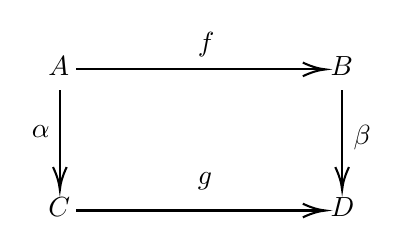
\begin{tikzpicture}[x=0.75pt,y=0.75pt,yscale=-1,xscale=1]
%uncomment if require: \path (0,476); %set diagram left start at 0, and has height of 476

%Straight Lines [id:da7570086255673307] 
\draw    (208,150) -- (326,150) ;
\draw [shift={(328,150)}, rotate = 180] [color={rgb, 255:red, 0; green, 0; blue, 0 }  ][line width=0.75]    (10.93,-3.29) .. controls (6.95,-1.4) and (3.31,-0.3) .. (0,0) .. controls (3.31,0.3) and (6.95,1.4) .. (10.93,3.29)   ;
%Straight Lines [id:da2086758955241419] 
\draw    (336,160) -- (336,206) ;
\draw [shift={(336,208)}, rotate = 270] [color={rgb, 255:red, 0; green, 0; blue, 0 }  ][line width=0.75]    (10.93,-3.29) .. controls (6.95,-1.4) and (3.31,-0.3) .. (0,0) .. controls (3.31,0.3) and (6.95,1.4) .. (10.93,3.29)   ;
%Straight Lines [id:da9244959521459397] 
\draw    (208,218) -- (326,218) ;
\draw [shift={(328,218)}, rotate = 180] [color={rgb, 255:red, 0; green, 0; blue, 0 }  ][line width=0.75]    (10.93,-3.29) .. controls (6.95,-1.4) and (3.31,-0.3) .. (0,0) .. controls (3.31,0.3) and (6.95,1.4) .. (10.93,3.29)   ;
%Straight Lines [id:da04532308225696924] 
\draw    (200,160) -- (200,206) ;
\draw [shift={(200,208)}, rotate = 270] [color={rgb, 255:red, 0; green, 0; blue, 0 }  ][line width=0.75]    (10.93,-3.29) .. controls (6.95,-1.4) and (3.31,-0.3) .. (0,0) .. controls (3.31,0.3) and (6.95,1.4) .. (10.93,3.29)   ;

% Text Node
\draw (193,142.4) node [anchor=north west][inner sep=0.75pt]    {$A$};
% Text Node
\draw (329,142.4) node [anchor=north west][inner sep=0.75pt]    {$B$};
% Text Node
\draw (193,210.4) node [anchor=north west][inner sep=0.75pt]    {$C$};
% Text Node
\draw (329,210.4) node [anchor=north west][inner sep=0.75pt]    {$D$};
% Text Node
\draw (265,130.4) node [anchor=north west][inner sep=0.75pt]    {$f$};
% Text Node
\draw (265,198.4) node [anchor=north west][inner sep=0.75pt]    {$g$};
% Text Node
\draw (185,175.4) node [anchor=north west][inner sep=0.75pt]    {$\alpha $};
% Text Node
\draw (340,175.4) node [anchor=north west][inner sep=0.75pt]    {$\beta $};


\end{tikzpicture}
\end{center}
\end{example}
\begin{definition}
Let $\mathcal{C}$ be a category and $\{A_i:i\in I\}$ a family of objects of $\mathcal{C}$. A \textbf{product} for the family $\{A_i:i\in I\}$ is an object $P$ of $\mathcal{C}$ together with a family of morphisms $\{\pi_i:P\to A_i:i\in I\}$ such that for any object $B$ and family of morphisms $\{\varphi_i:B\to A_i\}$, there is a unique morphism $\varphi:B\to P$ such that $\pi_i\circ\varphi=\varphi_i$ for all $i\in I$.
\end{definition}
We often denote the element $P=\prod_{i\in I}A_i$. We may rephrase the definition of product as that there exists a unique morphism $\varphi:B\to P$, such that the diagram for each $i\in I$
\begin{center}


\tikzset{every picture/.style={line width=0.75pt}} %set default line width to 0.75pt        

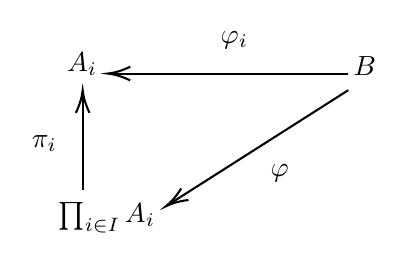
\begin{tikzpicture}[x=0.75pt,y=0.75pt,yscale=-1,xscale=1]
%uncomment if require: \path (0,476); %set diagram left start at 0, and has height of 476

%Straight Lines [id:da7917139115963452] 
\draw    (208,216) -- (208,170) ;
\draw [shift={(208,168)}, rotate = 90] [color={rgb, 255:red, 0; green, 0; blue, 0 }  ][line width=0.75]    (10.93,-3.29) .. controls (6.95,-1.4) and (3.31,-0.3) .. (0,0) .. controls (3.31,0.3) and (6.95,1.4) .. (10.93,3.29)   ;
%Straight Lines [id:da6002607042449972] 
\draw    (336,160) -- (222,160) ;
\draw [shift={(220,160)}, rotate = 360] [color={rgb, 255:red, 0; green, 0; blue, 0 }  ][line width=0.75]    (10.93,-3.29) .. controls (6.95,-1.4) and (3.31,-0.3) .. (0,0) .. controls (3.31,0.3) and (6.95,1.4) .. (10.93,3.29)   ;
%Straight Lines [id:da40319741776590323] 
\draw    (336,168) -- (249.69,222.93) ;
\draw [shift={(248,224)}, rotate = 327.53] [color={rgb, 255:red, 0; green, 0; blue, 0 }  ][line width=0.75]    (10.93,-3.29) .. controls (6.95,-1.4) and (3.31,-0.3) .. (0,0) .. controls (3.31,0.3) and (6.95,1.4) .. (10.93,3.29)   ;

% Text Node
\draw (199,148.4) node [anchor=north west][inner sep=0.75pt]    {$A_{i}$};
% Text Node
\draw (195,220.4) node [anchor=north west][inner sep=0.75pt]    {$\prod _{i\in I} A_{i}$};
% Text Node
\draw (337,150.4) node [anchor=north west][inner sep=0.75pt]    {$B$};
% Text Node
\draw (273,138.4) node [anchor=north west][inner sep=0.75pt]    {$\varphi _{i}$};
% Text Node
\draw (182,188.4) node [anchor=north west][inner sep=0.75pt]    {$\pi _{i}$};
% Text Node
\draw (297,202.4) node [anchor=north west][inner sep=0.75pt]    {$\varphi $};


\end{tikzpicture}
\end{center}
is commute.\par
A family of objects in a category need not have a product. In several familiar categories, however, products always exist. For example, in the category of sets the Cartesian product $\prod_{i\in I}A_i$ is a product of the family $\{A_i:i\in I\}$, which always exist. In the next section we will show that products exist in the category of groups.
\begin{theorem}
If $(P,\{\pi_i\})$ and $(Q,\{\psi_i\})$ are both products of the family $\{A_i:i\in I\}$ of objects of a category $\mathcal{C}$, then $P$ and $Q$ are equivalent.
\end{theorem}
\begin{proof}
Since $P$ and $Q$ are all products of $\{A_i:i\in I\}$, hence there exists morphisms $f$ and $g$ such that the following diagrams 
\begin{center}


\tikzset{every picture/.style={line width=0.75pt}} %set default line width to 0.75pt        

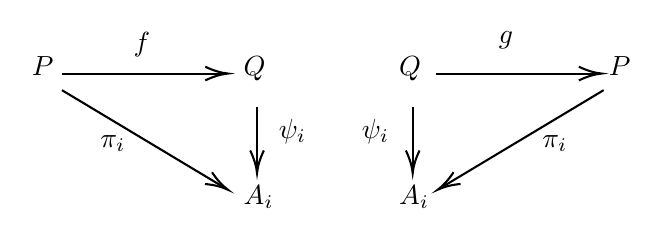
\begin{tikzpicture}[x=0.75pt,y=0.75pt,yscale=-1,xscale=1]
%uncomment if require: \path (0,476); %set diagram left start at 0, and has height of 476

%Straight Lines [id:da7225286591575897] 
\draw    (136,184) -- (214,184) ;
\draw [shift={(216,184)}, rotate = 180] [color={rgb, 255:red, 0; green, 0; blue, 0 }  ][line width=0.75]    (10.93,-3.29) .. controls (6.95,-1.4) and (3.31,-0.3) .. (0,0) .. controls (3.31,0.3) and (6.95,1.4) .. (10.93,3.29)   ;
%Straight Lines [id:da032279626256402905] 
\draw    (230,200) -- (230,230) ;
\draw [shift={(230,232)}, rotate = 270] [color={rgb, 255:red, 0; green, 0; blue, 0 }  ][line width=0.75]    (10.93,-3.29) .. controls (6.95,-1.4) and (3.31,-0.3) .. (0,0) .. controls (3.31,0.3) and (6.95,1.4) .. (10.93,3.29)   ;
%Straight Lines [id:da8049502306412264] 
\draw    (136,192) -- (214.29,238.97) ;
\draw [shift={(216,240)}, rotate = 210.96] [color={rgb, 255:red, 0; green, 0; blue, 0 }  ][line width=0.75]    (10.93,-3.29) .. controls (6.95,-1.4) and (3.31,-0.3) .. (0,0) .. controls (3.31,0.3) and (6.95,1.4) .. (10.93,3.29)   ;
%Straight Lines [id:da6416669281867011] 
\draw    (316,184) -- (394,184) ;
\draw [shift={(396,184)}, rotate = 180] [color={rgb, 255:red, 0; green, 0; blue, 0 }  ][line width=0.75]    (10.93,-3.29) .. controls (6.95,-1.4) and (3.31,-0.3) .. (0,0) .. controls (3.31,0.3) and (6.95,1.4) .. (10.93,3.29)   ;
%Straight Lines [id:da4963797883748118] 
\draw    (305,200) -- (305,230) ;
\draw [shift={(305,232)}, rotate = 270] [color={rgb, 255:red, 0; green, 0; blue, 0 }  ][line width=0.75]    (10.93,-3.29) .. controls (6.95,-1.4) and (3.31,-0.3) .. (0,0) .. controls (3.31,0.3) and (6.95,1.4) .. (10.93,3.29)   ;
%Straight Lines [id:da03213362948006537] 
\draw    (397,192) -- (318.71,238.97) ;
\draw [shift={(317,240)}, rotate = 329.04] [color={rgb, 255:red, 0; green, 0; blue, 0 }  ][line width=0.75]    (10.93,-3.29) .. controls (6.95,-1.4) and (3.31,-0.3) .. (0,0) .. controls (3.31,0.3) and (6.95,1.4) .. (10.93,3.29)   ;

% Text Node
\draw (120,174.4) node [anchor=north west][inner sep=0.75pt]    {$P$};
% Text Node
\draw (222,174.4) node [anchor=north west][inner sep=0.75pt]    {$Q$};
% Text Node
\draw (222,236.4) node [anchor=north west][inner sep=0.75pt]    {$A_{i}$};
% Text Node
\draw (169,162.4) node [anchor=north west][inner sep=0.75pt]    {$f$};
% Text Node
\draw (239,204.4) node [anchor=north west][inner sep=0.75pt]    {$\psi _{i}$};
% Text Node
\draw (153,212.4) node [anchor=north west][inner sep=0.75pt]    {$\pi _{i}$};
% Text Node
\draw (297,174.4) node [anchor=north west][inner sep=0.75pt]    {$Q$};
% Text Node
\draw (398,174.4) node [anchor=north west][inner sep=0.75pt]    {$P$};
% Text Node
\draw (297,236.4) node [anchor=north west][inner sep=0.75pt]    {$A_{i}$};
% Text Node
\draw (279,204.4) node [anchor=north west][inner sep=0.75pt]    {$\psi _{i}$};
% Text Node
\draw (345,162.4) node [anchor=north west][inner sep=0.75pt]    {$g$};
% Text Node
\draw (366,212.4) node [anchor=north west][inner sep=0.75pt]    {$\pi _{i}$};


\end{tikzpicture}
\end{center}
are commute for all $i\in I$. Now by composing these diagrams we get the following diagram:
\begin{center}


\tikzset{every picture/.style={line width=0.75pt}} %set default line width to 0.75pt        

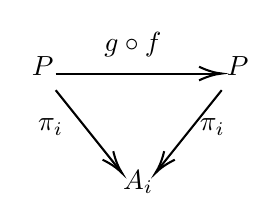
\begin{tikzpicture}[x=0.75pt,y=0.75pt,yscale=-1,xscale=1]
%uncomment if require: \path (0,476); %set diagram left start at 0, and has height of 476

%Straight Lines [id:da4312490537168616] 
\draw    (136,184) -- (214,184) ;
\draw [shift={(216,184)}, rotate = 180] [color={rgb, 255:red, 0; green, 0; blue, 0 }  ][line width=0.75]    (10.93,-3.29) .. controls (6.95,-1.4) and (3.31,-0.3) .. (0,0) .. controls (3.31,0.3) and (6.95,1.4) .. (10.93,3.29)   ;
%Straight Lines [id:da9269323080776339] 
\draw    (136,192) -- (166.75,230.44) ;
\draw [shift={(168,232)}, rotate = 231.34] [color={rgb, 255:red, 0; green, 0; blue, 0 }  ][line width=0.75]    (10.93,-3.29) .. controls (6.95,-1.4) and (3.31,-0.3) .. (0,0) .. controls (3.31,0.3) and (6.95,1.4) .. (10.93,3.29)   ;
%Straight Lines [id:da0759773200651006] 
\draw    (216,192) -- (185.25,230.44) ;
\draw [shift={(184,232)}, rotate = 308.66] [color={rgb, 255:red, 0; green, 0; blue, 0 }  ][line width=0.75]    (10.93,-3.29) .. controls (6.95,-1.4) and (3.31,-0.3) .. (0,0) .. controls (3.31,0.3) and (6.95,1.4) .. (10.93,3.29)   ;

% Text Node
\draw (123,174.4) node [anchor=north west][inner sep=0.75pt]    {$P$};
% Text Node
\draw (217,174.4) node [anchor=north west][inner sep=0.75pt]    {$P$};
% Text Node
\draw (167,229.4) node [anchor=north west][inner sep=0.75pt]    {$A_{i}$};
% Text Node
\draw (158,162.4) node [anchor=north west][inner sep=0.75pt]    {$g\circ f$};
% Text Node
\draw (126,204.4) node [anchor=north west][inner sep=0.75pt]    {$\pi _{i}$};
% Text Node
\draw (204,204.4) node [anchor=north west][inner sep=0.75pt]    {$\pi _{i}$};


\end{tikzpicture}
\end{center}
Thus $g\circ f:P\to P$ is a morphism such that $\pi_i\circ(g\circ f)=\pi_i$ for all $i\in I$. However by definition of a product, we know such morphism is unique and hence $g\circ f=1_P$. Similarly we know that $f\circ g=1_Q$ and hence $f:P\to Q$ is an equivalence.
\end{proof}
Since abstract categories involve only objects and morphisms, every statement about them has a dual statement, obtained by reversing all arrows(morphisms) in the original statement. For example, we know that the product can be state as the commuting diagram as follows:
\begin{center}


\tikzset{every picture/.style={line width=0.75pt}} %set default line width to 0.75pt        

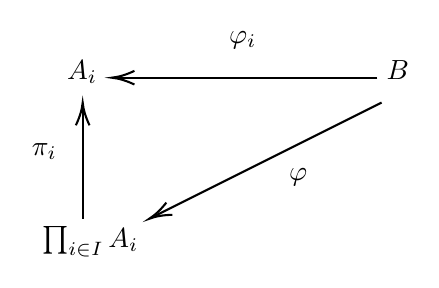
\begin{tikzpicture}[x=0.75pt,y=0.75pt,yscale=-1,xscale=1]
%uncomment if require: \path (0,476); %set diagram left start at 0, and has height of 476

%Straight Lines [id:da2649918540937004] 
\draw    (184,192) -- (184,138) ;
\draw [shift={(184,136)}, rotate = 90] [color={rgb, 255:red, 0; green, 0; blue, 0 }  ][line width=0.75]    (10.93,-3.29) .. controls (6.95,-1.4) and (3.31,-0.3) .. (0,0) .. controls (3.31,0.3) and (6.95,1.4) .. (10.93,3.29)   ;
%Straight Lines [id:da12188979211863638] 
\draw    (326,124) -- (200,124) ;
\draw [shift={(198,124)}, rotate = 360] [color={rgb, 255:red, 0; green, 0; blue, 0 }  ][line width=0.75]    (10.93,-3.29) .. controls (6.95,-1.4) and (3.31,-0.3) .. (0,0) .. controls (3.31,0.3) and (6.95,1.4) .. (10.93,3.29)   ;
%Straight Lines [id:da6877451403419319] 
\draw    (328,136) -- (217.79,191.11) ;
\draw [shift={(216,192)}, rotate = 333.43] [color={rgb, 255:red, 0; green, 0; blue, 0 }  ][line width=0.75]    (10.93,-3.29) .. controls (6.95,-1.4) and (3.31,-0.3) .. (0,0) .. controls (3.31,0.3) and (6.95,1.4) .. (10.93,3.29)   ;

% Text Node
\draw (175,114.4) node [anchor=north west][inner sep=0.75pt]    {$A_{i}$};
% Text Node
\draw (163,194.4) node [anchor=north west][inner sep=0.75pt]    {$\prod _{i\in I} A_{i}$};
% Text Node
\draw (329,114.4) node [anchor=north west][inner sep=0.75pt]    {$B$};
% Text Node
\draw (158,154.4) node [anchor=north west][inner sep=0.75pt]    {$\pi _{i}$};
% Text Node
\draw (253,100.4) node [anchor=north west][inner sep=0.75pt]    {$\varphi _{i}$};
% Text Node
\draw (282,166.4) node [anchor=north west][inner sep=0.75pt]    {$\varphi $};


\end{tikzpicture}
\end{center}
If we reverse all the arrows above, we get another commuting diagram: 
\begin{center}


\tikzset{every picture/.style={line width=0.75pt}} %set default line width to 0.75pt        

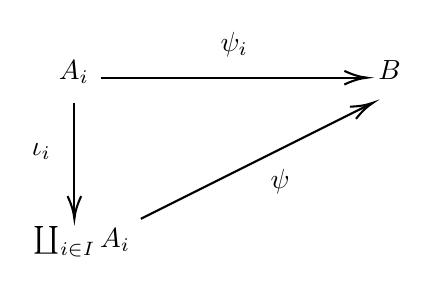
\begin{tikzpicture}[x=0.75pt,y=0.75pt,yscale=-1,xscale=1]
%uncomment if require: \path (0,476); %set diagram left start at 0, and has height of 476

%Straight Lines [id:da2649918540937004] 
\draw    (184,136) -- (184,190) ;
\draw [shift={(184,192)}, rotate = 270] [color={rgb, 255:red, 0; green, 0; blue, 0 }  ][line width=0.75]    (10.93,-3.29) .. controls (6.95,-1.4) and (3.31,-0.3) .. (0,0) .. controls (3.31,0.3) and (6.95,1.4) .. (10.93,3.29)   ;
%Straight Lines [id:da12188979211863638] 
\draw    (197,124) -- (323,124) ;
\draw [shift={(325,124)}, rotate = 180] [color={rgb, 255:red, 0; green, 0; blue, 0 }  ][line width=0.75]    (10.93,-3.29) .. controls (6.95,-1.4) and (3.31,-0.3) .. (0,0) .. controls (3.31,0.3) and (6.95,1.4) .. (10.93,3.29)   ;
%Straight Lines [id:da6877451403419319] 
\draw    (216,192) -- (326.21,136.89) ;
\draw [shift={(328,136)}, rotate = 153.43] [color={rgb, 255:red, 0; green, 0; blue, 0 }  ][line width=0.75]    (10.93,-3.29) .. controls (6.95,-1.4) and (3.31,-0.3) .. (0,0) .. controls (3.31,0.3) and (6.95,1.4) .. (10.93,3.29)   ;

% Text Node
\draw (175,114.4) node [anchor=north west][inner sep=0.75pt]    {$A_{i}$};
% Text Node
\draw (163,194.4) node [anchor=north west][inner sep=0.75pt]    {$\coprod _{i\in I} A_{i}$};
% Text Node
\draw (329,114.4) node [anchor=north west][inner sep=0.75pt]    {$B$};
% Text Node
\draw (162,154.4) node [anchor=north west][inner sep=0.75pt]    {$\iota _{i}$};
% Text Node
\draw (253,100.4) node [anchor=north west][inner sep=0.75pt]    {$\psi _{i}$};
% Text Node
\draw (277,166.4) node [anchor=north west][inner sep=0.75pt]    {$\psi $};


\end{tikzpicture}
\end{center}
From which we give the definition of coproducts:
\begin{definition}
A \textbf{coproduct} (or \textbf{sum}) for the family $\{A_i:i\in I\}$ of objects in a category $\mathcal{C}$ is an object $S$ of $\mathcal{C}$, together with a family of morphisms $\{\iota_i:A_i\to S\}$, such that for any object $B$ and family of morphisms $\{\psi_i:A_i\to B:i\in I\}$, there is a unique morphism $\psi:S\to B$ such that $\psi\circ\iota_i=\psi_i$ for all $i\in I$.
\end{definition}
By the same method used in theorem 2.55 one can proof that the coproduct is unique for a category $\mathcal{C}$. We skip the proof of this proposition.\par
In several of the categories mentioned above, every object in the category is in fact a set (usually with some additional structure) and every morphism in the category is a function on the "underlying sets". We formalize this idea in
\begin{definition}
A \textbf{concrete category} is a category $\mathcal{C}$ together with a function $\sigma$ that assigns to each object $A$ of $\mathcal{C}$ a set $\sigma(A)$(called the \textbf{underlying set} of $A$) in such a way that:\par
(i) every morphism $A\to B$ of $\mathcal{C}$ is a function on the underlying sets $\sigma(A)\to\sigma(B)$;\par
(ii) the identity morphism of each object $A$ of $\mathcal{C}$ is the identity function on the underlying set of $\sigma(A)$;\par
(iii) composition of morphisms in $\mathcal{C}$ agrees with the composition of functions on the underlying sets.
\end{definition}
Indeed, the function $\sigma$ has an effect to "forget" some structures of objects $A$ in the category $\mathcal{C}$. Actually such $\sigma$ is called a \textbf{forgetful functor}.\par
\begin{example}\em
The category of groups $\mathcal{G}$, equipped with the function that assigns to each group its underlying set in the usual sense, is a concrete category.
\end{example}
Concrete categories are frequently useful since one has available not only the properties of a category, but also certain properties of sets, subsets, etc. Since in virtually every concrete category we are interested in, the function $\sigma$ assigns to an object its underlying set in the usual sense, we shall denote both the object and its underlying set by the same symbol and omit any explicit reference to $\sigma$. There is little chance of confusion since we shall be careful in a concrete category $\mathcal{C}$ to distinguish morphisms of $\mathcal{C}$ and maps, which may not be a morphism on $\mathcal{C}$.
\begin{definition}
Let $F$ be an object in a concrete category $\mathcal{C}$. $X$ is a nonempty set, and $i:X\to F$ is a map (of sets). $F$ is \textbf{free on the set $X$} provided that for any object $A$ of $\mathcal{C}$ and map (of sets) $f:X\to A$, there exists a unique morphism $\overline{f}:F\to A$ in $\mathcal{C}$, such that $\overline{f}i=f$ (as a map of sets $X\to A$).
\end{definition}
Also this definition can be rephrased into a commute diagram:
\begin{center}


\tikzset{every picture/.style={line width=0.75pt}} %set default line width to 0.75pt        

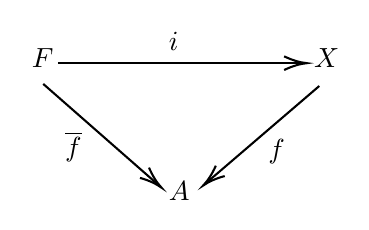
\begin{tikzpicture}[x=0.75pt,y=0.75pt,yscale=-1,xscale=1]
%uncomment if require: \path (0,476); %set diagram left start at 0, and has height of 476

%Straight Lines [id:da3029953557396716] 
\draw    (215,147) -- (333,147) ;
\draw [shift={(335,147)}, rotate = 180] [color={rgb, 255:red, 0; green, 0; blue, 0 }  ][line width=0.75]    (10.93,-3.29) .. controls (6.95,-1.4) and (3.31,-0.3) .. (0,0) .. controls (3.31,0.3) and (6.95,1.4) .. (10.93,3.29)   ;
%Straight Lines [id:da7623644977709794] 
\draw    (341,158) -- (286.52,204.7) ;
\draw [shift={(285,206)}, rotate = 319.4] [color={rgb, 255:red, 0; green, 0; blue, 0 }  ][line width=0.75]    (10.93,-3.29) .. controls (6.95,-1.4) and (3.31,-0.3) .. (0,0) .. controls (3.31,0.3) and (6.95,1.4) .. (10.93,3.29)   ;
%Straight Lines [id:da4655396103461529] 
\draw    (208,157) -- (263.5,205.68) ;
\draw [shift={(265,207)}, rotate = 221.26] [color={rgb, 255:red, 0; green, 0; blue, 0 }  ][line width=0.75]    (10.93,-3.29) .. controls (6.95,-1.4) and (3.31,-0.3) .. (0,0) .. controls (3.31,0.3) and (6.95,1.4) .. (10.93,3.29)   ;

% Text Node
\draw (201,138.4) node [anchor=north west][inner sep=0.75pt]    {$F$};
% Text Node
\draw (337,138.4) node [anchor=north west][inner sep=0.75pt]    {$X$};
% Text Node
\draw (267,202.4) node [anchor=north west][inner sep=0.75pt]    {$A$};
% Text Node
\draw (267,130.4) node [anchor=north west][inner sep=0.75pt]    {$i$};
% Text Node
\draw (315,182.4) node [anchor=north west][inner sep=0.75pt]    {$f$};
% Text Node
\draw (217,178.4) node [anchor=north west][inner sep=0.75pt]    {$\overline{f}$};


\end{tikzpicture}
\end{center}
We will give an example of free objects in section 9, where we will further study some properties of free groups. Now we show an essential fact about a free object $F$, which is, in order to define a morphism with domain $F$, it suffices to specify the image of the subset $i(X)$ as is seen in the following examples.\par
\begin{example}\em
Let $G$ be any group and $g\in G$. Then the map $\overline{f}:\mathbb{Z}\to G$ defined by $\overline{f}(n)=g^n$ is easily to be the unique homomorphism $\mathbb{Z}\to G$ such that $1\mapsto g$. Consequently, if $X=\{1\}$ and $i:X\to\mathbb{Z}$ be the inclusion map, then $\mathbb{Z}$ is free on $X$ in the category of groups. In other words, to determine a unique homomorphism from $\mathbb{Z}$ to $G$, we need only specify the image of $1\in\mathbb{Z}$, which is $i(X)$. 
\end{example}
\begin{theorem}
If $\mathcal{C}$ is a concrete category, $F$ and $F^\prime$ are objects of $\mathcal{C}$ such that $F$ is free on $X$ and $F^\prime$ is free on $X^\prime$, if $|X|=|X^\prime|$, then $F$ and $F^\prime$ are equivalent.
\end{theorem}
\begin{proof}
Since $F$ and $F^\prime$ are free on $X$ and $X^\prime$ separately and $|X|=|X^\prime|$, we may define a bijection $f:X\to X^\prime$ and maps $i:X\to F$, $j:X^\prime\to F^\prime$. Consider the map $jf:X\to F^\prime$. Since $F$ is free on $X$, there exists a morphism $\varphi:F\to F^\prime$ such that the diagram 
\begin{center}


\tikzset{every picture/.style={line width=0.75pt}} %set default line width to 0.75pt        

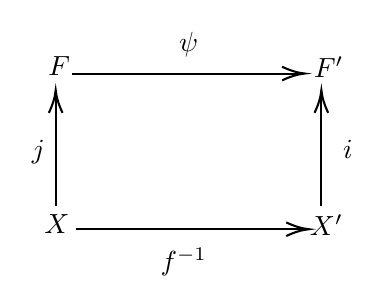
\begin{tikzpicture}[x=0.75pt,y=0.75pt,yscale=-1,xscale=1]
%uncomment if require: \path (0,476); %set diagram left start at 0, and has height of 476

%Straight Lines [id:da9276054517030092] 
\draw    (216,144) -- (326,144) ;
\draw [shift={(328,144)}, rotate = 180] [color={rgb, 255:red, 0; green, 0; blue, 0 }  ][line width=0.75]    (10.93,-3.29) .. controls (6.95,-1.4) and (3.31,-0.3) .. (0,0) .. controls (3.31,0.3) and (6.95,1.4) .. (10.93,3.29)   ;
%Straight Lines [id:da34128781451565393] 
\draw    (208,208) -- (208,154) ;
\draw [shift={(208,152)}, rotate = 90] [color={rgb, 255:red, 0; green, 0; blue, 0 }  ][line width=0.75]    (10.93,-3.29) .. controls (6.95,-1.4) and (3.31,-0.3) .. (0,0) .. controls (3.31,0.3) and (6.95,1.4) .. (10.93,3.29)   ;
%Straight Lines [id:da047714159922908506] 
\draw    (218,219) -- (328,219) ;
\draw [shift={(330,219)}, rotate = 180] [color={rgb, 255:red, 0; green, 0; blue, 0 }  ][line width=0.75]    (10.93,-3.29) .. controls (6.95,-1.4) and (3.31,-0.3) .. (0,0) .. controls (3.31,0.3) and (6.95,1.4) .. (10.93,3.29)   ;
%Straight Lines [id:da6552908409349356] 
\draw    (336,208) -- (336,154) ;
\draw [shift={(336,152)}, rotate = 90] [color={rgb, 255:red, 0; green, 0; blue, 0 }  ][line width=0.75]    (10.93,-3.29) .. controls (6.95,-1.4) and (3.31,-0.3) .. (0,0) .. controls (3.31,0.3) and (6.95,1.4) .. (10.93,3.29)   ;

% Text Node
\draw (201,210.4) node [anchor=north west][inner sep=0.75pt]    {$X$};
% Text Node
\draw (329,210.4) node [anchor=north west][inner sep=0.75pt]    {$X^{\prime }$};
% Text Node
\draw (203,134.4) node [anchor=north west][inner sep=0.75pt]    {$F$};
% Text Node
\draw (331,134.4) node [anchor=north west][inner sep=0.75pt]    {$F^{\prime }$};
% Text Node
\draw (257,226.4) node [anchor=north west][inner sep=0.75pt]    {$f^{-1}$};
% Text Node
\draw (345,174.4) node [anchor=north west][inner sep=0.75pt]    {$i$};
% Text Node
\draw (195,174.4) node [anchor=north west][inner sep=0.75pt]    {$j$};
% Text Node
\draw (266,122.4) node [anchor=north west][inner sep=0.75pt]    {$\psi $};


\end{tikzpicture}
\end{center}
is commutative. Similarly, we have another commute diagram as follow:
\begin{center}


\tikzset{every picture/.style={line width=0.75pt}} %set default line width to 0.75pt        

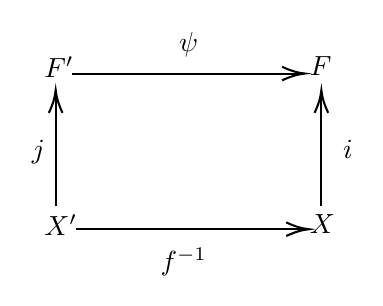
\begin{tikzpicture}[x=0.75pt,y=0.75pt,yscale=-1,xscale=1]
%uncomment if require: \path (0,476); %set diagram left start at 0, and has height of 476

%Straight Lines [id:da9276054517030092] 
\draw    (216,144) -- (326,144) ;
\draw [shift={(328,144)}, rotate = 180] [color={rgb, 255:red, 0; green, 0; blue, 0 }  ][line width=0.75]    (10.93,-3.29) .. controls (6.95,-1.4) and (3.31,-0.3) .. (0,0) .. controls (3.31,0.3) and (6.95,1.4) .. (10.93,3.29)   ;
%Straight Lines [id:da34128781451565393] 
\draw    (208,208) -- (208,154) ;
\draw [shift={(208,152)}, rotate = 90] [color={rgb, 255:red, 0; green, 0; blue, 0 }  ][line width=0.75]    (10.93,-3.29) .. controls (6.95,-1.4) and (3.31,-0.3) .. (0,0) .. controls (3.31,0.3) and (6.95,1.4) .. (10.93,3.29)   ;
%Straight Lines [id:da047714159922908506] 
\draw    (218,219) -- (328,219) ;
\draw [shift={(330,219)}, rotate = 180] [color={rgb, 255:red, 0; green, 0; blue, 0 }  ][line width=0.75]    (10.93,-3.29) .. controls (6.95,-1.4) and (3.31,-0.3) .. (0,0) .. controls (3.31,0.3) and (6.95,1.4) .. (10.93,3.29)   ;
%Straight Lines [id:da6552908409349356] 
\draw    (336,208) -- (336,154) ;
\draw [shift={(336,152)}, rotate = 90] [color={rgb, 255:red, 0; green, 0; blue, 0 }  ][line width=0.75]    (10.93,-3.29) .. controls (6.95,-1.4) and (3.31,-0.3) .. (0,0) .. controls (3.31,0.3) and (6.95,1.4) .. (10.93,3.29)   ;

% Text Node
\draw (329,210.4) node [anchor=north west][inner sep=0.75pt]    {$X$};
% Text Node
\draw (201,210.4) node [anchor=north west][inner sep=0.75pt]    {$X^{\prime }$};
% Text Node
\draw (329,134.4) node [anchor=north west][inner sep=0.75pt]    {$F$};
% Text Node
\draw (201,134.4) node [anchor=north west][inner sep=0.75pt]    {$F^{\prime }$};
% Text Node
\draw (257,226.4) node [anchor=north west][inner sep=0.75pt]    {$f^{-1}$};
% Text Node
\draw (345,174.4) node [anchor=north west][inner sep=0.75pt]    {$i$};
% Text Node
\draw (195,174.4) node [anchor=north west][inner sep=0.75pt]    {$j$};
% Text Node
\draw (266,122.4) node [anchor=north west][inner sep=0.75pt]    {$\psi $};


\end{tikzpicture}
\end{center}
Combining these two diagram together, we have 
\begin{center}


\tikzset{every picture/.style={line width=0.75pt}} %set default line width to 0.75pt        

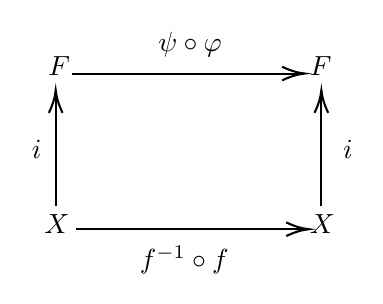
\begin{tikzpicture}[x=0.75pt,y=0.75pt,yscale=-1,xscale=1]
%uncomment if require: \path (0,476); %set diagram left start at 0, and has height of 476

%Straight Lines [id:da9276054517030092] 
\draw    (216,144) -- (326,144) ;
\draw [shift={(328,144)}, rotate = 180] [color={rgb, 255:red, 0; green, 0; blue, 0 }  ][line width=0.75]    (10.93,-3.29) .. controls (6.95,-1.4) and (3.31,-0.3) .. (0,0) .. controls (3.31,0.3) and (6.95,1.4) .. (10.93,3.29)   ;
%Straight Lines [id:da34128781451565393] 
\draw    (208,208) -- (208,154) ;
\draw [shift={(208,152)}, rotate = 90] [color={rgb, 255:red, 0; green, 0; blue, 0 }  ][line width=0.75]    (10.93,-3.29) .. controls (6.95,-1.4) and (3.31,-0.3) .. (0,0) .. controls (3.31,0.3) and (6.95,1.4) .. (10.93,3.29)   ;
%Straight Lines [id:da047714159922908506] 
\draw    (218,219) -- (328,219) ;
\draw [shift={(330,219)}, rotate = 180] [color={rgb, 255:red, 0; green, 0; blue, 0 }  ][line width=0.75]    (10.93,-3.29) .. controls (6.95,-1.4) and (3.31,-0.3) .. (0,0) .. controls (3.31,0.3) and (6.95,1.4) .. (10.93,3.29)   ;
%Straight Lines [id:da6552908409349356] 
\draw    (336,208) -- (336,154) ;
\draw [shift={(336,152)}, rotate = 90] [color={rgb, 255:red, 0; green, 0; blue, 0 }  ][line width=0.75]    (10.93,-3.29) .. controls (6.95,-1.4) and (3.31,-0.3) .. (0,0) .. controls (3.31,0.3) and (6.95,1.4) .. (10.93,3.29)   ;

% Text Node
\draw (201,210.4) node [anchor=north west][inner sep=0.75pt]    {$X$};
% Text Node
\draw (203,134.4) node [anchor=north west][inner sep=0.75pt]    {$F$};
% Text Node
\draw (329,134.4) node [anchor=north west][inner sep=0.75pt]    {$F$};
% Text Node
\draw (247,225.4) node [anchor=north west][inner sep=0.75pt]    {$f^{-1} \circ f$};
% Text Node
\draw (345,174.4) node [anchor=north west][inner sep=0.75pt]    {$i$};
% Text Node
\draw (195,174.4) node [anchor=north west][inner sep=0.75pt]    {$i$};
% Text Node
\draw (256,122.4) node [anchor=north west][inner sep=0.75pt]    {$\psi \circ \varphi $};
% Text Node
\draw (329,210.4) node [anchor=north west][inner sep=0.75pt]    {$X$};


\end{tikzpicture}
\end{center}
Hence $(\psi\circ\varphi)i=i1_X=i$. But $1_Fi=i$, thus by uniqueness of free objects we must have $\psi\circ\varphi=1_F$. A similar argument shows that $\varphi\circ\psi=1_{F^\prime}$. Therefore $F$ is equivalent to $F^\prime$.
\end{proof}
Products, coproducts, and free objects are all defined via \textbf{universal mapping properties}, that is, in terms of the existence of certain uniquely determined morphisms. We formalize the definition as follows:
\begin{definition}
An object $I$ in a category $\mathcal{C}$ is said to be \textbf{universal} (or \textbf{initial}) if for each object $C$ of $\mathcal{C}$ there exists one and only one morphism $I\to C$. An object $T$ in a category $\mathcal{C}$ is said to be \textbf{couniversal} (or \textbf{terminal}) if for each object $C$ of $\mathcal{C}$ there exists one and only one morphism $C\to T$.
\end{definition}
We shall now show that any two universal (couniversal) objects in a category $\mathcal{C}$ are equivalent.
\begin{theorem}
Any two universal (couniversal) objects in a category $\mathcal{C}$ are equivalent.
\end{theorem}
\begin{proof}
Let $I$ and $J$ be universal objects in $\mathcal{C}$. Since $I$ is universal, there is a unique morphism $f:I\to J$. Similarly, there is a unique morphism $g:J\to I$. The composition $g\circ f:I\to I$ is a morphism of $\mathcal{C}$. But $1_I:I\to I$ is also a morphism, then by uniqueness we know that $g\circ f=1_I$. Similarly we have $f\circ g=1_J$ and hence $f$ and $g$ are equivalent. The proof for couniversal objects is analogous.
\end{proof}
Note that categories is a language rather than technique, so we list only a few exercises and we proceed our study for more examples and usage of this language.
\begin{center}
\begin{large}
    \textbf{Exercises for 2.7}
\end{large}
\end{center}
\begin{problem}\em
A pointed set is a pair $(S,x)$ with $S$ a set and $x\in S$. A morphism of pointed sets $(S,x)\mapsto(S^\prime,x^\prime)$ is a triple $(f,x,x^\prime)$ where $f:S\to S^\prime$ is a function satisfies $f(x)=x^\prime$. Show that points sets form a category.
\end{problem}
\begin{proof}
It is clear that for each $(S_1,x_1)$ and $(S_2,x_2)$, the set $\hom((S_1,x_1),(S_2,x_2))$ are disjoint. Also the identity and associativity is trivial. Now we proof that 
$$\hom((S_1,x_1),(S_2,x_2))\times\hom((S_2,x_2),(S_3,x_3))=\hom((S_1,x_1),(S_3,x_3)).$$
To show this, we define the composition $(f,x_1,x_2)\in\hom((S_1,x_1),(S_2,x_2))$ and $(g,x_2,x_3)\in\hom((S_2,x_2),(S_3,x_3))$ as the usual composition of functions, therefore $gf(x_1)=g(x_2)=x_3$ and hence $(gf,x_1,x_3)\in\hom((S_1,x_1),(S_3,x_3))$, which finished our proof.
\end{proof}
\begin{problem}\em
If $f:A\to B$ is an equivalence in a category $\mathcal{C}$ and $g:B\to A$ satisfies $f\circ g=1_B$ and $g\circ f=1_A$, show that $g$ is unique.
\end{problem}
\begin{proof}
Suppose $g$ and $g^\prime$ both satisfy the condition, we proof that $g=g^\prime$. Observed that 
$$
g=1_B\circ g=\left( g^{\prime}\circ f \right) \circ g=g^{\prime}\circ \left( f\circ g \right) =g^{\prime}\circ 1_A=g^{\prime},
$$
hence $g=g^\prime$ and we finished our proof.
\end{proof}
\begin{problem}\em
In the category of groups $\mathcal{G}$, show that the group $G_1\times G_2$ together with the homomorphisms $\pi_1:G_1\times G_2\to G_1$ and $\pi_2:G_1\times G_2\to G_2$ is a product for $\{G_1,G_2\}$.
\end{problem}
\begin{proof}
We first proof that for a class of sets $\{A_i:i\in I\}$ the Cartesian product $\prod_{i\in I}A_i$ is the product in the category $\mathcal{S}$. Let $\pi_i:\prod_{i\in I}A_i\to A_i$, now we show that for an arbitrarily chosen set $C$ and a class of maps $\{\varphi_i:C\to A_i\}$, there exists a unique $\varphi:B\to\prod_{i\in I}A_i$ such that $\varphi_i=\pi_i\circ\varphi$. Let $\varphi$ given by $b\mapsto f_b$, where $f_b(i)=\varphi_i(b)$. It is easy to verify that such $\varphi$ satisfy $\varphi_i=\pi_i\circ\varphi$. Now if there exists another $\varphi^\prime$, observed that 
$$
\varphi ^{\prime}\left( b \right) \left( t \right) =\pi _i\circ \varphi ^{\prime}\left( b \right) =\varphi _i\left( b \right) =f_b\left( i \right) =\varphi \left( b \right) \left( i \right) ,
$$
hence we finished our proof.\par
For this exercise, we simply need to show that $\varphi$ we defined above is a homomorphism, which is easy when observed that 
$$
\varphi \left( ab \right) \left( i \right) =f_{ab}\left( i \right) =\varphi _i\left( ab \right) =\varphi _i\left( a \right) \varphi _i\left( b \right) =f_a\left( i \right) f_b\left( i \right) =\varphi \left( a \right) \varphi \left( b \right) \left( i \right) ,
$$
and hence we finished our proof.
\end{proof}
\begin{problem}\em
Every family $\{A_i:i\in I\}$ in the category of sets has a coproduct.
\end{problem}
\begin{proof}
We define the \textbf{disjoint union} of the set $A_i$ as follows:
$$
\bigsqcup_{i\in I}{A_i}=\left\{ \left( a,i \right) \in \left( \bigcup_{i\in I}{A_i} \right) \times I:a\in A_i \right\} .
$$
Now we define the map $A_i\to\bigsqcup_{i\in I}A_i$ given by $a\mapsto(a,i)$. We proof that $\bigsqcup_{i\in I}{A_i}$ is a coproduct of $\{A_i:i\in I\}$ in the category of sets.\par
For another set $C$ and a class of $\{\psi_i:A_i\to C:i\in I\}$, we define $\psi$ by $(a,i)\mapsto\psi_i(a)$, therefore it is easy to verify that $\psi$ satisfy the condition and unique.
\end{proof}
\subsection{Direct Products and Direct Sums}
In this section we study the product in the category of groups and the coproduct in the category of abelian groups.\par
We begin by extending the definition of the direct product $G\times H$ of groups $G$ and $H$, which we once defined in example 2.3, to an arbitrarily chosen family of groups $\{G_i:i\in I\}$. Define a binary operation on the Cartesian product $\prod_{i\in I}G_i$, which we defined in exercise 2.89. If $f,g\in\prod_{i\in I}G_i$, then $fg$ is given by $i\mapsto f(i)g(i)$. Since $G_i$ is a group, $f(i)g(i)\in G_i$ for all $i\in I$, thence $fg\in\prod_{i\in I}G_i$. $\prod_{i\in I}G_i$, together with the binary operation defined above, is called the \textbf{direct product} of the family of groups $\{G_i:i\in I\}$. If $I$ is finite, we may denote $\prod_{i\in I}G_i=G_1\times G_2\times\cdots\times G_n$. In additive notation, the \textbf{complete direct sum} is denoted as $\bigoplus_{i\in I}G_i$ or $G_1\oplus G_2\oplus\cdots\oplus G_n$ when $I$ is finite. We have shown in exercise 2.89 that $\prod_{i\in I}G_i$ is a product in the category of groups, now we study more properties of direct product.
\begin{proposition}
If $\{G_i:i\in I\}$ is a family of group, then the direct product $\prod_{i\in I}G_i$ is a group, and for each $k\in I$, the map $\pi_k:\prod_{i\in I}G_i\to G_k$ given by $f\mapsto f(k)$ is an epimorphism of groups.
\end{proposition}
\begin{proof}
Clearly for $f,g,h\in\prod_{i\in I}G_i$, $(fg)h=f(gh)$, hence $\prod_{i\in I}G_i$ is a semi-group. Observed that $1\in\prod_{i\in I}G_i$ given by $i\mapsto e_i$, where $e_i$ is the identity element of $G_i$ satisfies $1f=f$, $g1=g$, hence $1$ is the identity element of $\prod_{i\in I}G_i$ and hence a monoid. Now for an arbitrarily chosen $f\in\prod_{i\in I}G_i$, we define $g$ by $i\mapsto(f(i))^{-1}$, which is well-defined since $G_i$ is a group for all $i\in I$. Then $fg=gf=1$, hence $g$ is the inverse of $f$ and $\prod_{i\in I}G_i$ is a group. For each $a\in G_k$, there exists an element $f\in\prod_{i\in I}G_i$ given by $f(k)=a$ and $f(j)=e_j$ where $j\ne k$, hence $\pi_k$ is an epimorphism.
\end{proof}
\begin{note}\em
The map $\pi_k$ here is called the \textbf{canonical projections} of the direct product.
\end{note}
Note that since the direct product of abelian groups is clearly abelian, it follows that the direct product of abelian groups is a product in the category of abelian groups also.\par
\begin{definition}
The \textbf{weak direct product} or the \textbf{external direct product} of a family of groups, denoted as ${\prod}^W_{i\in I}G_i$, is the set of all $f\in\prod_{i\in I}G_i$ such that $f(i)=e_i$, the identity in $G_i$, for all but a finite number of $i\in I$. If all the groups $G_i$ are additive abelian, ${\prod}^W_{i\in I}G_i$ is called the \textbf{external direct sum} and denoted as $\sum_{i\in I}G_i$.
\end{definition}
If $I$ is finite, the weak direct product coincides with the direct product. In any case, we have the following proposition:
\begin{proposition}
If $\{G_i:i\in I\}$ is a family of groups, then\par
(i) ${\prod}^W_{i\in I}G_i$ is a normal subgroup of $\prod_{i\in I}G_i$.\par
(ii) for each $k\in I$, the map $\iota_k:G_k\to{\prod}^W_{i\in I}G_i$ given by $\iota_k(a)=\{a_i\}_{i\in I}$, where $a_i=e$ for $i\ne k$ and $a_k=a$, is a monomorphism of groups.\par
(iii) for each $i\in I$, $\iota_i(G_i)$ is a normal subgroup of $\prod_{i\in I}G_i$.
\end{proposition}
\begin{proof}
(i) Let $f\in{\prod}^W_{i\in I}G_i$ and $f\in\prod_{i\in I}G_i$. Now we consider $gfg^{-1}$, which satisfies $gfg^{-1}(i)=g_if_ig_i^{-1}=g_ig_i^{-1}=e_i$ for all but a finite number of $i$, hence $gfg^{-1}\in{\prod}^W_{i\in I}G_i$ and hence normal in $\prod_{i\in I}G_i$.
(ii) Let $\iota_k(a)=\iota_k(b)$. Therefore the image $\{a_i\}_{i\in I}$ and $\{b_i\}_{i\in I}$ satisfies $a_i=b_i=e$ when $i\ne k$ and $a_k=b_k=a=b$ when $i=k$, hence $a=b$, therefore $\iota_k$ is a monomorphism.\par
(iii) Let $f\in\iota_k(G_k)$ and $g\in\prod_{k\in I}G_k$, therefore 
$$
gfg^{-1}\left( i \right) =g_if_ig_{i}^{-1}=\begin{cases}
	g_ieg_{i}^{-1}=g_ig_{i}^{-1}=e,i\ne k,\\
	g_kf_kg_{k}^{-1}\in G_k,i=k,\\
\end{cases}
$$
hence $gfg^{-1}\in\iota_k(G_k)$ and hence $\iota_k(G_k)\lhd\prod_{i\in I}G_i$.
\end{proof}
\begin{note}\em
The maps $\iota_k$ here is called the \textbf{canonical injection}.
\end{note}
\begin{theorem}
Let $\{A_i:i\in I\}$ be a family of abelian groups written additively. If $B$ is an abelian group and $\{\psi:A_i\to B:i\in I\}$ a family of homomorphisms, then there is a unique homomorphism $\psi:\sum_{i\in I}A_i\to B$ such that $\psi\iota_i=\psi_i$ for all $i\in I$ and this property determine $\sum_{i\in I}A_i$ uniquely up to isomorphism. In other words, $\sum_{i\in I}A_i$ is a coproduct in the category of abelian groups.
\end{theorem}
\begin{proof}
By definition of the external direct sum we know that for each $f\in\sum_{i\in I}A_i$, there is only finite number of $k$ such that $f(k)\ne 0$. We denote such $f(k)$ as $a_k$ and let $\psi(f)=\sum_{k}a_k$. Clearly $\psi$ satisfies the condition $\psi\iota_i=\psi_i$ and it is a homomorphism. Now if $\xi$ is another homomorphism that satisfies $\xi\iota_i=\psi_i$, observed that 
\begin{small}
$$
\xi \left( \left\{ a_i \right\} \right) =\xi \left( \sum_k{\iota _k\left( a \right)} \right) =\sum_k{\xi \iota _k\left( a_k \right)}=\sum_k{\psi _k\left( a_k \right)}=\sum_k{\psi \iota _k\left( a_k \right)}=\psi \left( \sum_k{\iota _k\left( a_k \right)} \right) =\psi \left( \left\{ a_i \right\} \right) ,
$$
\end{small}
hence $\xi=\psi$, which shows that $\psi$ is unique. Therefore $\sum A_i$ is a coproduct in the category of abelian groups and hence is determined up to isomorphism by theorem 2.55 and duality.
\end{proof}
Now we investigate conditions under which a group $G$ is isomorphic to the weak product of a family of its subgroups.
\begin{theorem}
Let $\{N_i:i\in I\}$ be a family of normal subgroups of a group $G$ such that $G=\left<\bigcup_{i\in I}\right>$, and for each $k\in I$, $N_k\cap\left<\bigcup_{i\ne k}\right>=\left<e\right>$. Then $G\cong{\prod}^W_{i\in I}G_i$.
\end{theorem}
\begin{proof}
Let $\{a_i\}\in{\prod}^W_{i\in I}G_i$, then by definition of a weak direct product we know that there are only finite $a_k$ such that $a_k\ne e$. Hence $\{a_i\}=\prod_{k}a_k$. Now we define $\psi:{\prod}^W_{i\in I}G_i\to G$ by $\{a_i\}\mapsto\prod_{k}a_k$. Note that for $a_i\in N_i$ and $a_j\in N_j$ $a_i$ and $a_j$ are commute which we have proved in theorem 2.32, and now we proof that $\psi$ is an isomorphism. First, it is easy to verify that $\psi$ is a homomorphism. Let $a\in G$, by definition of $G$ we may let $a=\prod_{i\in I}a_i$. Now take all $a_k\ne e$ and observed that 
$$
\psi \left( \prod_k{\iota _k\left( a_k \right)} \right) =\prod_k{\psi \iota _k\left( a_k \right)}=\prod_k{a_k}=a,
$$
hence $\psi$ is an epimorphism. Now we show that $\mathrm{Ker}\psi=\left<e\right>$ and hence a monomorphism. Let $\psi \left( \left\{ a_i \right\} \right) =\prod_k{a_k}=e$. Then for all $a_{k_0}$ we have $\prod_k{a_k}=a_{k_0}\prod_{k\ne k_0}{a_k}=e$ and hence 
$$
a_{k_0}^{-1}=\prod_{k\ne k_0}{a_k}\in N_{k_0}\cap \left< \bigcup_{i\ne k_0}{N_i} \right> =\left< e \right> ,
$$
which is $a_{k_0}=e$. Observed that it generally holds and hence $\{a_i\}=e$, therefore $\psi$ is an isomorphism and $G\cong{\prod}^W_{i\in I}G_i$.
\end{proof}
\begin{corollary}
If $N_1,N_2,\cdots,N_r$ are normal subgroups of a group $G$ such that $G=N_1N_2\cdots N_r$ and for each $1\le k\le r$, $N_k\cap(N_1\cdots N_{k-1}N_{k+1}\cdots N_r)=\left<e\right>$, then $G\cong N_1\times N_2\times\cdots\times N_r$.
\end{corollary}
This is an immediate consequence of theorem 2.66 since $I$ can be finite. We skip the proof of this corollary.\par
As another easy corollary of theorem 2.66 we have the following characterization of internal weak direct products.
\begin{theorem}
Let $\{N_i:i\in I\}$ be a family of normal subgroups of a group $G$. $G$ is the internal weak direct product of the family $\{N_iLi\in I\}$ if and only if every non-identity element of $G$ is a unique product $a_{i_1}a_{i_2}\cdots a_{i_n}$ with $i_1,i_2,\cdots,i_n$ distinct elements of $I$ and $e\ne a_{i_k}\in N_{i_k}$ for each $k=1,2,\cdots,n$.
\end{theorem}
\begin{proof}
By theorem 2.66 we know that the internal subgroup of $\{N_i:i\in I\}$ is isomorphic to ${\prod}^W_{i\in I}N_i$, and the theorem immediately follows by the definition of external direct product.
\end{proof}
There are some distinctions between the internal direct product and external direct product. For example, by definition of the internal direct product $G$, each $N_i$ is the subgroup of $G$, then $G$ is isomorphic to ${\prod}^W_{i\in I}N_i$. However, $N_i$ doesn't necessarily be the subgroup of ${\prod}^W_{i\in I}N_i$. In fact, only copies of them are isomorphic to ${\prod}^W_{i\in I}N_i$(namely $\iota_i(N_i)$, we will discuss it later in exercises). Practically speaking, this distinction is not very important and the adjectives "internal" and "external" may be omitted when no confusion is possible to occur.\par
We denote $G={\prod}^w_{i\in I}N_i$ as the internal weak direct product of the family of its subgroups $\{N_i:i\in I\}$.
\begin{theorem}
Let $\{f_i:G_i\to H_i:i\in I\}$ be a family of homomorphisms of groups and let $f=\prod_{i\in I}f_i$ be the map $\prod_{i\in I}G_i\to\prod_{i\in I}H_i$ given by $\{a_i\}\mapsto\{f_i(a_i)\}$. Then $f$ is a homomorphism of groups such that $f\left({\prod}^W_{i\in I}G_i\right)\subset{\prod}^W_{i\in I}H_i$, $\mathrm{Ker}f=\prod_{i\in I}\mathrm{Ker}f_i$ and $\mathrm{Im}f=\prod_{i\in I}\mathrm{Im}f_i$. Consequently $f$ is a monomorphism [resp. epimorphism] if and only if each $f_i$ is.
\end{theorem}
\begin{proof}
We first proof that $f$ is a homomorphism, which only need to observe that 
$$
f\left( \left\{ a_ib_i \right\} \right) =f_i\left( a_ib_i \right) =f_i\left( a_i \right) f_i\left( b_i \right) =f\left( \left\{ a_i \right\} \right) f\left( \left\{ b_i \right\} \right) .
$$
Now it is trivial that $f\left({\prod}^W_{i\in I}G_i\right)\subset{\prod}^W_{i\in I}H_i$ and we show $\mathrm{Ker}f=\prod_{i\in I}\mathrm{Ker}f_i$, $\mathrm{Im}f=\prod_{i\in I}\mathrm{Im}f_i$. In fact, if $\{a_i\}\in\prod_{i\in I}\mathrm{Ker}f_i$, then $f\left( \left\{ a_i \right\} \right) =\left\{ f_i\left( a_i \right) \right\} =\left< e \right> $ and hence $\mathrm{Ker}f\supset \prod_{i\in I}{\mathrm{Ker}f_i}$. Conversely, if $\{a_i\}\in\mathrm{Ker}f$, then $f\left( \left\{ a_i \right\} \right) =\left\{ f_i\left( a_i \right) \right\} =\left< e \right> $ for all $i\in I$, whence $\left\{ a_i \right\} \in \prod_{i\in I}{\mathrm{Ker}f_i}$. Hence $\mathrm{Ker}f=\prod_{i\in I}\mathrm{Ker}f_i$. Similarly one may verify that $\mathrm{Im}f=\prod_{i\in I}\mathrm{Im}f_i$.
\end{proof}
\begin{corollary}
Let $\{G_i:i\in I\}$ and $\{N_i:i\in I\}$ be two families of groups such that $N_i\lhd G_i$ for each $i\in I$.\par
(i)$\prod_{i\in I}{N_i}\lhd \prod_{i\in I}{G_i}$ and $\prod_{i\in I}{G_i}/\prod_{i\in I}{N_i}\cong \prod_{i\in I}{\left( G_i/N_i \right)}$.\par
(ii)${\prod}^W_{i\in I}{N_i}\lhd {\prod}^W_{i\in I}{G_i}$ and ${\prod}^W_{i\in I}{G_i}/{\prod}^W_{i\in I}{N_i}\cong {\prod}^W_{i\in I}{\left( G_i/N_i \right)}$.
\end{corollary}
\begin{proof}
We only proof (i) and (ii) can be proved similarly.\par
Define the canonical epimorphism $\pi_i:G_i\to G_i/N_i$. Then the product $\pi =\prod_{i\in I}{\pi _i}:\prod_{i\in I}{G_i}\rightarrow \prod_{i\in I}{\left( G_i/N_i \right)}$ is an epimorphism with kernel $\mathrm{Ker}\pi=\prod_{i\in I}N_i$. Hence by the First Isomorphism Theorem we have $\prod_{i\in I}{N_i}\lhd \prod_{i\in I}{G_i}$ and $\prod_{i\in I}{G_i}/\prod_{i\in I}{N_i}\cong \prod_{i\in I}{\left( G_i/N_i \right)}$.
\end{proof}
\begin{center}
\begin{large}
    \textbf{Exercises for 2.8}
\end{large}
\end{center}
\begin{problem}\em
Show that $S_3$ is not the direct product of any family of its proper groups. The same is true for $\mathbb{Z}_{p^n}$ and $\mathbb{Z}$.
\end{problem}
\begin{proof}
Our proof depend on an observation that if $A$ and $B$ are abelian, then so is $A\times B$. Now we consider the subgroups of $S_3$. By Lagrange's Theorem, it has an order either $2$ or $3$, which are all prime. Hence subgroups of $S_3$ are all abelian, so if $S_3$ is the direct product of some of its subgroups, it must be abelian, which is a contradiction!\par
The proof for $\mathbb{Z}_{p^n}$ is similar since $\mathbb{Z}_{p^n}$ has its subgroups of the form $\left<p^k\right>$ where $1\le k\le n-1$. Consider any product $\left<p^i\right>\times\left<p^j\right>$. Let $G=\mathbb{Z}_{p^{i_1}}\times\mathbb{Z}_{p^{i_2}}\times\cdots\times\mathbb{Z}_{p^{i_m}}$, then both $\left<(p^{i-1},0,\cdots,0)\right>$ and $\left<(0,0,\cdots,p^{j-1})\right>$ are both subgroups with order $p$. However, this can't be true since by exercise 2.35 we know that such subgroup should be unique. Therefore $G$ is not the internal subgroup of $\mathbb{Z}_{p^n}$.\par
The group $\mathbb{Z}$ is cyclic. However, any product of its subgroups contains a subgroup $m\mathbb{Z}\times n\mathbb{Z}$, which is not cyclic. Hence $\mathbb{Z}$ is not the direct product of some of its subgroups by the same reason.
\end{proof}
\begin{problem}\em
Give an example of groups $H_i,K_j$ such that $H_1\times H_2\cong K_1\times K_2$, but $H_i\not\cong K_j$ for any $i,j=1,2$.
\end{problem}
\begin{proof}
Consider the example $\mathbb{Z}_2\times\mathbb{Z}_6$ and $(\mathbb{Z}_2\times\mathbb{Z}_2)\times\mathbb{Z}_3$. We first show that $\mathbb{Z}_2\times\mathbb{Z}_6\cong(\mathbb{Z}_2\times\mathbb{Z}_2)\times\mathbb{Z}_3$. Observed that the element $(1,1)\in\mathbb{Z}_2\times\mathbb{Z}_3$ generates the whole $\mathbb{Z}_2\times\mathbb{Z}_3$, therefore $\mathbb{Z}_2\times\mathbb{Z}_3\cong\mathbb{Z}_6$. Now define the map $(0,1)\mapsto((0,1)),0$ and $(1,0)\mapsto((1,0),0)$. Since the generators determined the whole map, we know that it is an isomorphism. However, no isomorphism exists in $\mathbb{Z}_2,\mathbb{Z}_6,\mathbb{Z}_2\times\mathbb{Z}_2$ and $\mathbb{Z}_3$.
\end{proof}
\begin{note}\em
This example shows that the decomposition of a group may not be unique.
\end{note}
\begin{problem}\em
Let $G$ be an additive abelian group with subgroups $H$ and $K$. Show that $G\cong H\oplus K$ if and only if there are homomorphisms $H\underset{\iota _1}{\overset{\pi _1}{\leftrightarrows}}G\underset{\iota _2}{\overset{\pi _2}{\leftrightarrows}}K$ such that $\pi_1\iota_1=1_H,\pi_2\iota_2=1_K,\pi_1\iota_2=0$ and $\pi_2\iota_1=0$, where $0$ is the map sending every element onto zero element, and $\iota_1\pi_1(x)+\iota_2\pi_2(x)=x$ for all $x\in G$.
\end{problem}
\begin{proof}
If $G\cong H\oplus K$, then for all $x\in G$, we may write $x=(h,k)$ where $h\in H$ and $k\in K$. Hence we define $\pi_1:(h,k)\mapsto h,\pi_2:(h,k)\mapsto k$ and $\iota_1:h\mapsto(h,0),\iota_2:k\mapsto(0,k)$, then it is easy to verify that these maps are homomorphisms and satisfy the condition shown in exercise. Conversely, since $\pi_1\iota_1=1_H$, we know that $\iota_1$ is injective and $\pi_1$ is surjective. Hence $H$ is embedded in $G$, that is, $H^\prime=\iota_1(H)<G$. Given $h^\prime\in H^\prime$, there is a unique $h\in H$ such that $\iota_1(h)=h^\prime$, hence $H\cong H^\prime$. Similarly we have $K\cong H^\prime$. Now that $\iota_1\pi_1(x)+\iota_2\pi_2(x)=x$ hence $G=H^\prime+K^\prime$. We define $f:G\to H\oplus K$ by $h^\prime+k^\prime\mapsto(h,k)$, which is easy to see is an isomorphism, hence $G\cong H\oplus H$.
\end{proof}
\begin{problem}\em
Let $G,H$ be cyclic groups. Then $G\times H$ is cyclic if and only if $(|G|,|H|)=1$.
\end{problem}
\begin{proof}
If $G\times H$ is cyclic but $(|G|,|H|)\ne 1$. Then we may take elements from $G$ and $H$, denote $g,h$, have the same order. Now consider $G\times H$. Since $(g,e_H)$ and $(e_G,h)$ are both elements of $G\times H$, then $\left<(g,e_H\right>$ and $\left<e_G,h\right>$ have the same order and all subgroups of $G\times H$, which contradicts to the fact that $G\times H$ is cyclic. Conversely, if $(|G|,|H|)=1$, then suppose $|G|=p$ and $|H|=q$, we know by exercise 2.31 that $G\times H$ is an abelian group that contains an element of order $[m,n]$. Observed that $mn=[m,n](m,n)=[m,n]$ and $|G\times H|=|G|\times|H|=mn$, we know that $G\times H$ is cyclic since it can be generated by one element.
\end{proof}
\begin{problem}\em
Every finite generated abelian group $G\ne\left<e\right>$ in which every element (except $e$) has order $p$ ($p$ prime) is isomorphic to $\mathbb{Z}_p\oplus\mathbb{Z}_p\oplus\cdots\oplus\mathbb{Z}_p$.
\end{problem}
\begin{proof}
Let $A=\{a_1,a_2,\cdots,a_n\}$ be the collection of all generators of $G$, which satisfy $\left< A\setminus \left\{ a_k \right\} \right> \ne G$ for all $k\in\{1,2,\cdots,n\}$. Denote $\left<a_k\right>=N_k$, then $N_k\lhd G$. We now show that $G$ is the direct product of $N_k,k=1,2,\cdots,n$. First observed that 
$A\subset (N_1\cup N_2\cup \cdots \cup N_n)$, hence $G\subset \left< N_1\cup N_2\cup \cdots \cup N_n \right> $. The converse condition is trivial and hence $G=\left< N_1\cup N_2\cup \cdots \cup N_n \right> $. Now we show that 
$$N_k\cap \left( N_1\cup \cdots \cup N_{k-1}\cup N_{k+1}\cup \cdots \cup N_n \right) =0$$ 
for all $k\in\{1,2,\cdots,n\}$. Observed that 
$$N_k\cap \left( N_1\cup \cdots \cup N_{k-1}\cup N_{k+1}\cup \cdots \cup N_n \right) $$
is the subset of $N_k$ and $N_k$ has an order $p$, which is prime, therefore 
$$N_k\cap \left( N_1\cup \cdots \cup N_{k-1}\cup N_{k+1}\cup \cdots \cup N_n \right) =N_k\ \text{or}\ 0.$$
If the first, $\left< N_1\cup \cdots \cup N_{k-1}\cup N_{k+1}\cup \cdots \cup N_n \right> $ generates the whole $G$, which contradict to the definition of $A$. Hence $N_k\cap \left( N_1\cup \cdots \cup N_{k-1}\cup N_{k+1}\cup \cdots \cup N_n \right) =0 $ and therefore we finished our proof.
\end{proof}
\begin{problem}\em
Let $H,K,N$ be nontrivial normal subgroups of a group $G$ and suppose $G=H\times K$. Prove that $N$ is in the center of $G$ or $N$ intersects one of $H,K$ nontrivially. Give examples to show that both possibilities can actually occur when $G$ is not abelian.
\end{problem}
\begin{proof}
Suppose $N\cap H=N\cap K=\left<e\right>$. Now take $n\in N$ and $k\in K$. Since $N$ is normal in $G$, we know that $knk^{-1}\in N$. Also we know that $nk^{-1}n^{-1}\in K$ since $k$ is normal in $G$. This shows that $knk^{-1}n^{-1}\in N\cap K=\left<e\right>$ and hence $kn=nk$. Similarly we have $hn=nh$ and therefore $Z(G)=G$, we finished our proof.\par
Now we give an example that both two condition may be true when $G$ is not abelian. Consider $D_2\cong\mathbb{Z}_2\oplus\mathbb{Z}_2$. We denote $D_2=\left<a\right>\times\left<b\right>$ and it has a subgroup $\left<ab\right>$ which does not intersect either product. However, since the group is abelian then every element is contained in the center. Then consider $D_6$. We observed that $D_6=\left<a^3\right>\times\left<a^2,b\right>\cong\mathbb{Z}_2\oplus D_3$, where $\left<a^3\right>\cap\left<a^2,b\right>=\left<e\right>$.
\end{proof}
\begin{problem}\em
Corollary 2.67 is false if one of the $N_i$ is not normal.
\end{problem}
\begin{problem}\em
If a group $G$ is the (internal) direct product of its subgroups $H,K$, then $H\cong G/K$ and $K\cong G/H$.
\end{problem}
\begin{proof}
Consider the canonical projection $\pi_H:G\to H$ and $\pi_K:G\to K$. We have shown that $\mathrm{Ker}\pi_K=H$, therefore by the First Isomorphism Theorem we have $G/\mathrm{Ker}\pi_K\cong\mathrm{Im}\pi_K$. However, it is easy to verify $\pi_K$ is an epimorphism and hence $\mathrm{Im}\pi_K=K$, therefore $G/H\cong K$. Analogously we have $G/K\cong H$.
\end{proof}
\begin{problem}\em
If $\{G_i:i\in I\}$ is a family of groups, then ${\prod}^w_{i\in I}G_i$ is the internal weak product of its subgroups $\{\iota_i(G_i):i\in I\}$.
\end{problem}
\begin{proof}
We have shown that $\iota_i(G_i)$ is normal in ${\prod}^w_{i\in I}G_i$. Now we show that 
$$
\iota _i\left( G_i \right) \cap \left( \iota _1\left( G_1 \right) \cup \cdots \cup \iota _{i-1}\left( G_{i-1} \right) \cup \iota _{i+1}\left( G_{i+1} \right) \cup \cdots \cup \iota _n\left( G_n \right) \right) =\left< e \right> .
$$
In fact we know that the map $\iota _i:G_i\rightarrow {\prod}^w_{i\in I}{G_i}$ is an embedding that 
$$\iota _i\left( G_i \right) =\left( e_1,\cdots ,e_{i-1},G_i,e_{i+1},\cdots ,e_n \right) ,$$
hence
$$
\iota _i\left( G_i \right) \cap \left( \iota _1\left( G_1 \right) \cup \cdots \cup \iota _{i-1}\left( G_{i-1} \right) \cup \iota _{i+1}\left( G_{i+1} \right) \cup \cdots \cup \iota _n\left( G_n \right) \right) =\left< e \right> .
$$
Then the statement follows by the fact that $
{\prod}^w_{i\in I}{G_i}=\left< \bigcup_{i\in I}{\iota _i\left( G_i \right)} \right> $.
\end{proof}
\begin{problem}\em
Let $\{N_i:i\in I\}$ is a family of subgroups of a group $G$. Then $G$ is the internal weak product of $\{N_i:i\in I\}$ if and only if:\par
(i) $a_ia_j=a_ja_i$ for all $i\ne j$ and $a_i\in N_i,a_j\in N_j$.\par
(ii) every non-identity element of $G$ is uniquely a product $a_{i_1}\cdots a_{i_n}$, where $i_1,i_2,\cdots,i_n$ are distinct elements of $I$ and $e\ne a_{i_k}$ for each $k$.
\end{problem}
\begin{proof}
By definition of an internal weak direct product we know that each $N_i$ is the normal subgroup of $G$. Then the statement immediately follows by theorem 2.32 and theorem 2.68. Conversely, by theorem 2.68 it suffices to show that each $N_i$ is normal in $G$, which is trivial when observed that for all $n_i\in N_i$ and $g\in G$, by (ii) we write $g=a_{i_1}\cdots a_{i_k}$, we have 
$$
gn_ig^{-1}=n_{i_1}n_{i_2}\cdots n_{i_n}n_in_{i_n}^{-1}n_{i_{n-1}}^{-1}\cdots n_{i_1}^{-1}=\left( n_{i_1}n_{i_1}^{-1} \right) \left( n_{i_2}n_{i_2}^{-1} \right) \cdots \left( n_{i_n}n_{i_n}^{-1} \right) n_i=n_i\in N_i,
$$
by which we finished our proof.
\end{proof}
\begin{problem}\em
Let $\{G_i:i\in I\}$ be a family of groups and $J\subset I$. The map $\alpha:\prod_{j\in J}G_j\to\prod_{i\in I}G_i$ given by $\{a_i\}\mapsto\{b_i\}$, where $b_j=a_j$ for $j\in J$ and $b_i=e_i$ for $i\notin J$, is a monomorphism of groups and $\prod_{i\in I}G_i/\alpha\left(\prod_{j\in J}G_j\right)\cong\prod_{i\in I\setminus J}G_i$.
\end{problem}
\begin{proof}
It is easy to verify that $\alpha$ is a monomorphism, we now proof $\prod_{i\in I}G_i/\alpha\left(\prod_{j\in J}G_j\right)\cong\prod_{i\in I\setminus J}G_i$. Define $\beta :\prod_{i\in I}{G_i}\rightarrow \prod_{i\in I\setminus J}{G_i}$ by $\{a_i\}\mapsto e$ if $\{a_i\}\in\prod_{j\in J}G_j$, otherwise $\{a_i\}\mapsto\{a_i\}$. It is easy to verify that $\beta$ is a homomorphism and $\mathrm{Ker}\beta=\alpha\left(\prod_{i\in I}G_i\right)$. Therefore by the First Isomorphism Theorem we have $\prod_{i\in I}G_i/\alpha\left(\prod_{j\in J}G_j\right)\cong\prod_{i\in I\setminus J}G_i$.
\end{proof}
\subsection{Free Groups, Free Products, Generators and Relations}
We shall show that free objects exists in the category of groups, and we shall use these to develop a method of describing groups in terms of "generators and relations". In addition, we indicate how to construct coproduct (free product) in the category of groups.\par
We now construct a free group on a given group $X$. If $X=\emptyset$, then $F$ is trivially $\left<e\right>$. Otherwise we consider the sequence $x_1x_2\cdots x_n\in F$, here $x_i\in X,i=1,2,\cdots,n$. In order $F$ to be a group, there must be an inverse for such an element in $F$. Hence we define a set $X^{-1}$ disjoint from $X$, such that $|X|=|X^{-1}|$. Hence there is a bijection $x\mapsto x^{-1}$ from $X$ to $X^{-1}$. Now choose an element $1$ out of $X\cup X^{-1}$. We say the sequence $x_1x_2\cdots x_n\cdots$ is a \textbf{word}, if there exists an index $k$ such that $a_j=1$ when $j\ge k$. The constant sequence $11\cdots1\cdots$ is denoted as $1$. A word $x_1x_2\cdots x_n$ is \textbf{reduced}, if \par
(i) for all $x\in X$, $x$ and $x^{-1}$ are not adjacent. That is, if $x_k=x$, then $x_{k+1}\ne x^{-1}$ and vice versa.\par
(ii) $a_k=1$ implies $a_j=1$ for all $j\ge k$.\par
Every reduced word has the form $x_1^{\lambda_1}x_2^{\lambda_2}\cdots x_n^{\lambda_n}$, where $x_i\in X$ and $\lambda_i=1$ or $-1$. Observed that $x_{1}^{\delta _1}x_{2}^{\delta _2}\cdots x_{n}^{\delta _n}=y_{1}^{\lambda _1}y_{2}^{\lambda _2}\cdots y_{m}^{\lambda _m}$ if and only if $m=n$, $x_i=y_i$ and $\delta_i=\lambda_i$. We now define the binary product as follows (in order that the product of two reduced words is reduced):
$$
\left( x_{1}^{\delta _1}x_{2}^{\delta _2}\cdots x_{n}^{\delta _n} \right) \left( y_{1}^{\lambda _1}y_{2}^{\lambda _2}\cdots y_{m}^{\lambda _m} \right) =\begin{cases}
	x_{1}^{\delta _1}x_{2}^{\delta _2}\cdots x_{n-k}^{\delta _{n-k}}y_{k+1}^{\lambda _{k+1}}y_{k+2}^{\lambda _{k+2}}\cdots y_{m}^{\lambda _m},k<m,\\
	y_{n+1}^{\lambda _{n+1}}y_{n+2}^{\lambda _{n+2}}\cdots y_{m}^{\lambda _m},k=m<n,\\
	1,k=m=n,\\
\end{cases}
$$
here $k$ is the largest integer such that $x_{n-j}^{\delta_{m-j}}=y_{j+1}^{-\lambda_{j+1}}$ for $j=1,2,\cdots,k-1$.
\begin{theorem}
If $X$ is a nonempty set and $F=F(X)$ is the set of all reduced words on $X$, then $F$ is a group under the binary operation defined above and $F=\left<X\right>$.
\end{theorem}
\begin{proof}
By definition of $F$ we know that $F$ has an identity element $1$ and for each $w\in F$ there is an inverse element $w^{-1}$. Now we show that elements in $F$ is associative. For each $x\in X$ and $\delta=-1$ or $1$, we define the map $|x^\delta|:F\to F$ given by 
$$
\left| x^{\delta} \right|\left( x_{1}^{\delta _1}x_{2}^{\delta _2}\cdots x_{n}^{\delta _n} \right) =\begin{cases}
	x^{\delta}x_{1}^{\delta _1}x_{2}^{\delta _2}\cdots x_{n}^{\delta _n},x^{\delta}x_{1}^{\delta _1}\ne 1,\\
	x_{2}^{\delta _2}\cdots x_{n}^{\delta _n},x^{\delta}x_1^{\delta_1}=1,\\
\end{cases}
$$
Since $|x||x^{-1}|=|x^{-1}||x|=1_F$, we know that every $|x^\delta|$ is a permutation of $F$. Let $F_0$ be the subgroup generated by $\{|x|:x\in X\}$. Now we define a map $\varphi:F\to F_0$ by $1\mapsto 1_F$ and $x_{1}^{\delta _1}x_{2}^{\delta _2}\cdots x_{n}^{\delta _n}\mapsto \left| x_{1}^{\delta _1} \right|\left| x_{2}^{\delta _2} \right|\cdots \left| x_{n}^{\delta _n} \right|$. We first show that it is a homomorphism. Observed that 
$$
\varphi \left( w_1w_2 \right) =\left| w_1w_2 \right|=\left| w_1 \right|\left| w_2 \right|=\varphi \left( w_1 \right) \varphi \left( w_2 \right) 
$$
hence $\varphi$ is a homomorphism. Clearly $\varphi$ is surjective. Then by definition of $\varphi$ that $1\mapsto 1_F$, hence $\mathrm{Ker}\varphi=1$ and hence injective. Therefore $\varphi$ is an isomorphism and hence $F\cong F_0$. Elements in $F_0$ is associative since $F_0$ is a group, therefore elements in $F$ is associative and we finished our proof.
\end{proof}
\begin{note}\em
The proof method above is called the \textbf{van der Waerden trick}.
\end{note}
\begin{definition}
The group $F=F(X)$ is called the \textbf{free group on the set $X$}.
\end{definition}
Here we explain the terminology "free".
\begin{theorem}
Let $F$ be the free group on a set $X$ and $\iota:X\to F$ is the inclusion map. If $G$ is a group and $f:X\to G$ a map of sets, then there exists a unique homomorphism of groups $\overline{f}:F\to G$ such that $\overline{f}\iota=f$.
\end{theorem}
\begin{proof}
We define the map $\overline{f}:F\to G$ by $\overline{f}(1)=e_G$ and 
$$\overline{f}\left( x_{1}^{\delta _1}x_{2}^{\delta _2}\cdots x_{n}^{\delta _n} \right) =f^{\delta _1}\left( x_1 \right) f^{\delta _2}\left( x_2 \right) \cdots f^{\delta _n}\left( x_n \right) .$$
We first proof that $\overline{f}$ is a homomorphism. Observed that 
$$
\begin{aligned}
\overline{f}\left( x_{1}^{\delta _1}x_{2}^{\delta _2}\cdots x_{n}^{\delta _n}y_{1}^{\lambda _1}y_{2}^{\lambda _2}\cdots y_{m}^{\lambda _m} \right) &=f^{\delta _1}\left( x_1 \right) f^{\delta _2}\left( x_2 \right) \cdots f^{\delta _n}\left( x_n \right) f^{\lambda _1}\left( y_1 \right) f^{\lambda _2}\left( y_2 \right) \cdots f^{\lambda _m}\left( y_m \right) \\
&=\overline{f}\left( x_{1}^{\delta _1}x_{2}^{\delta _2}\cdots x_{n}^{\delta _n} \right) \overline{f}\left( y_{1}^{\lambda _1}y_{2}^{\lambda _2}\cdots y_{m}^{\lambda _m} \right) ,
\end{aligned}
$$
hence $\overline{f}$ is a homomorphism. Now we show that $\overline{f}\iota=f$, which we observed that for all $x\in X$, $\iota(x)=x$, hence $\overline{f}\iota(x)=\overline{f}(x)=f(x)$, therefore $\overline{f}\iota=f$. Now if there is another homomorphism $g$ such that $g\iota=f$, we show that $g=\overline{f}$ by 
$$
\begin{aligned}
g\left( x_{1}^{\delta _1}x_{2}^{\delta _2}\cdots x_{n}^{\delta _n} \right) &=g\left( x_{1}^{\delta _1} \right) g\left( x_{2}^{\delta _2} \right) \cdots g\left( x_{n}^{\delta _n} \right)\\
&=g^{\delta _1}\left( x_1 \right) g^{\delta _2}\left( x_2 \right) \cdots g^{\delta _n}\left( x_n \right)=g\iota ^{\delta _1}\left( x_1 \right) g\iota ^{\delta _2}\left( x_2 \right) \cdots g\iota ^{\delta _n}\left( x_n \right)\\
&=f^{\delta _1}\left( x_1 \right) f^{\delta _2}\left( x_2 \right) \cdots f^{\delta _n}\left( x_n \right) =\overline{f}\left( x_{1}^{\delta _1}x_{2}^{\delta _2}\cdots x_{n}^{\delta _n} \right) ,
\end{aligned}
$$
hence we finished our proof.
\end{proof}
\begin{note}\em
In other words, $F$ is a free object on the set $X$ in the category of groups.
\end{note}
\begin{corollary}
Every group $G$ is isomorphic to quotient group of a free group.
\end{corollary}
\begin{proof}
By theorem 2.73 we know that the map $\overline{f}$ is an epimorphism, hence by the First Isomorphism Theorem we know that $G\cong F/\mathrm{Ker}\overline{f}$.
\end{proof}
By corollary 2.74 we know that in order to determine a group $G$, it suffices to determine $F,X$ and $\mathrm{Ker}\overline{f}=N$. However $F$ is determined up to isomorphism by $X$, and $N$ is determined by the homomorphism $\mathrm{Ker}\overline{f}$. Now if $w=x_1^{\delta_1}x_2^{\delta_2}\cdots x_n^{\delta_n}$ is a generator of $N$, then under the epimorphism $x_1^{\delta_1}x_2^{\delta_2}\cdots x_n^{\delta_n}=e$. We call the equation $x_1^{\delta_1}x_2^{\delta_2}\cdots x_n^{\delta_n}=e$ a \textbf{relation} of generators $x_i$ on $G$. Clearly a group can be determined by a set $X$ of generators and a suitable set $R$ of relations. This description is not unique, since there are many choices of $X$ and $R$.\par
Conversely, we may ask given a set $X$ and $Y$ of reduced words on the element of $X$, does there exists a group $G$ such that $G$ is generated by $X$ and the relations $w=e,w\in Y$ are all valid? We will see that the statement is true, providing one allows for the possibility that in the group $G$ the elements of $X$ may not all be distinct. For example, let $a,b\in X$ and $ab^{-1}\in Y$. Then every group $G$ containing $a$ and $b$ and satisfying $ab^{-1}=e$ must have $a=b$.\par
We now construct the group as follows. Let $F$ be the free group on $X$ and $N$ be the normal group generated by $Y$ (which is the intersection of all normal groups in $F$ that contains $Y$). Let $G$ be the quotient group $F/N$ and identify $X$ with its image in $F/N$ under the map $X\subset F\to F/N$. Then $G$ is a group generated by $X$ and for all $w\in Y$, 
$$
w=x_{1}^{\delta _1}x_{2}^{\delta _2}\cdots x_{n}^{\delta _n}\in Y\Rightarrow x_{1}^{\delta _1}x_{2}^{\delta _2}\cdots x_{n}^{\delta _n}\in N\Rightarrow x_{1}^{\delta _1}Nx_{2}^{\delta _2}N\cdots x_{n}^{\delta _n}N=N,
$$
hence $w=e$ in $G$.\par
\begin{definition}
Let $X$ be a set and $Y$ be a set of reduced words on $X$. A group $G$ is said to be the \textbf{group defined by the generators $x\in X$ and relations $w=e(w\in Y)$} provided $G\cong F/N$, where $F$ is the free group of $X$ and $N$ be the normal subgroup of $F$ generated by $Y$. One says that $(X\mid Y)$ is the \textbf{presentation} of $G$.
\end{definition}
The preceding discussion shows that the group defined by given generators and relations always exists. Furthermore it is the largest possible such group in the following sense.
\begin{theorem}(Van Dyck)
Let $X$ be a set, $Y$ a set of reduced words on $X$ and $G$ the group defined by the generators $x\in X$ and relations $w=e,w\in Y$. If $H$ is any group such that $H=\left<X\right>$ and $H$ satisfies all the relations $w=e(w\in Y)$, then there is an epimorphism $G\to H$.
\end{theorem}
\begin{note}\em
The elements of $Y$ are being interpreted as words in $X$, products in $G$ and products in $H$ as the context indicates.
\end{note}
\begin{proof}
If $F$ is the free group on $X$ then the inclusion map $X\to H$ induces an epimorphism $\varphi:F\to H$ by corollary 2.74. Since $H$ satisfies $w=e$ for all $w\in Y$, we know that $Y\subset\mathrm{Ker}\varphi$. Consequently, the normal subgroup generated by $Y$ is contained in $\mathrm{Ker}\phi$. By Corollary 2.37 we know that $F/N\cong H/0$. Hence $G\cong F/N\cong H/0\cong H$ is an epimorphism.
\end{proof}
The following examples defined by generators and relations illustrate the sort of ad hoc arguments that are often the only way of investigating a given presentation. When convenient, we shall use exponential notation for words. For example, we write $x^2y^{-3}$ rather than $x^1x^1y^{-1}y^{-1}y^{-1}$.
\begin{example}\em
Let $G$ be the group defined by generators $a,b$ and relations $a^4=e,a^2b^{-2}=e$ and $abab^{-1}=e$. Since the group $Q_8$ satisfy all these conditions, then there is an epimorphism $G\to Q_8$ and hence $|G|\ge|Q_8|$. Conversely, let $F$ be the free group on $\{a,b\}$ and $N$ be the normal subgroup of $F$ generated by $\{a^4,a^2b^{-2},abab^{-1}\}$, one may verify that elements of $F/N$ has the form $a^ib^jN$, where $i=0,1,2,3$ and $j=0,1$. Hence $|G|=|F/N|\le 8$ and therefore $G\cong Q_4$.
\end{example}
\begin{example}\em
By theorem 2.52 we know that the group defined by generators $a,b$ and relations $a^n=e,b^2=e$ and $abab=e$, here $n\ge 3$, is isomorphic to the dihedral group $D_n$.
\end{example}
\begin{example}\em
The free group $F$ on a set $X$ is the group defined by the generators $x\in X$ and no relations. The terminology "free" arises from the fact that $F$ is relation-free.
\end{example}
We close this section with a brief discussion of coproducts (free products) in the category of groups. One may observe that the process is similar to the construction of free groups.\par
Given a family of groups $\{G_i:i\in I\}$ we may assume without loss of generality that $G_i$ are disjoint. Let $X=\bigcup_{i\in I}G_i$ and let $\{1\}$ be a one-element set disjoint from $X$. A \textbf{word} on $X$ is any sequence $x_1x_2\cdots x_n\cdots$ such that $a_i\in X\cup\{1\}$ and for some $n\in N$, $a_i=1$ for all $i\ge n$. A word is said to be \textbf{reduced}, if provided\par
(i) no $a_i\in X$ is the identity element in $G_j$;\par
(ii) for all $i,j\ge 1$, $a_i$ and $a_{i+1}$ are not in the same group $G_k$;\par
(iii) $a_k=1$ implies $a_i=1$ for all $i\ge k$.\par
In particular $1=11\cdots 1\cdots$ is reduced. Now let ${\prod}^*_{i\in I}G_i$ be the set of all reduced words on $X$. ${\prod}^*_{i\in I}G_i$ forms a group, called the \textbf{free product} of the family $\{G_i:i\in I\}$, under the binary operation defined as follows. $1$ is the identity element and the product of two reduced words is defined as that in free groups. That is, product of two words are a joint while guaranteeing the product is also a reduced word. Finally, for each $k\in I$ the map $\iota_k:G_k\to{\prod}^*_{i\in I}G_i$ given by $e\mapsto 1$ and $a\mapsto a$ is a monomorphism of groups. Consequently, we sometimes identify $G_k$ with is isomorphic image in ${\prod}^*_{i\in I}G_i$.
\begin{theorem}
Let $\{G_i:i\in I\}$ be a family of groups and ${\prod}^*_{i\in I}G_i$ be the free product of $\{G_i:i\in I\}$. If $\{\psi_i:i\in I\}$ is a family of group homomorphisms, then there exists a unique homomorphism $\psi:{\prod}^*_{i\in I}G_i\to H$ such that $\psi\iota_i=\psi_i$ for all $i\in I$ and this property determined ${\prod}^*_{i\in I}G_i$ up to isomorphism. In other words, ${\prod}^*_{i\in I}G_i$ is a coproduct in the category of groups.
\end{theorem}
\begin{proof}
We define the map $\psi$ by $\psi(x_1x_2\cdots x_n)=\psi_{i_1}(x_1)\psi_{i_2}(x_2)\cdots\psi_{i_n}(x_n)$, where $x_k\in G_{i_k}$. Now we show that $\psi$ is a homomorphism and $\psi\iota_i=\psi_i$. First observed that 
$$
\begin{aligned}
\psi \left( x_1x_2\cdots x_ny_1y_2\cdots y_m \right) &=\psi _{i_1}\left( x_1 \right) \psi _{i_2}\left( x_2 \right) \cdots \psi _{i_n}\left( x_n \right) \psi _{j_1}\left( y_1 \right) \psi _{j_2}\left( y_2 \right) \cdots \psi _{j_m}\left( y_m \right) \\
&=\psi \left( x_1x_2\cdots x_n \right) \psi \left( y_1y_2\cdots y_m \right) ,
\end{aligned}
$$
hence $\psi$ is a homomorphism. Then for all $x_i\in G_i$, we have 
$$
\psi \iota _i\left( x_i \right) =\psi \left( x_i \right) =\psi _i\left( x_i \right) ,
$$
hence $\psi\iota_i=\psi_i$. Now if there is another homomorphism $\varphi$ satisfies $\varphi\iota_i=\psi_i$, we have 
$$
\begin{aligned}
\varphi \left( x_1x_2\cdots x_n \right) =\varphi \left( x_1 \right) \varphi \left( x_2 \right) \cdots \varphi \left( x_n \right) &=\varphi \iota _{i_1}\left( x_1 \right) \iota _{i_2}\varphi \left( x_2 \right) \cdots \varphi \iota _{i_n}\left( x_n \right) \\
&=\psi _{i_1}\left( x_1 \right) \psi _{i_2}\left( x_2 \right) \cdots \psi _{i_n}\left( x_n \right) =\psi \left( x_1x_2\cdots x_n \right) ,
\end{aligned}
$$
hence $\psi$ is unique. Therefore ${\prod}^*_{i\in I}G_i$ is a coproduct of $\{G_i:i\in I\}$.
\end{proof}
\begin{center}
\begin{large}
    \textbf{Exercises for 2.9}
\end{large}
\end{center}
\begin{problem}\em
Every non-identity element in a free group $F$ has infinite order.
\end{problem}
\begin{proof}
If not, let $a\in F$ and $a$ has a finite order. Then $a^m=e$ for some $m\in\mathbb{Z}$, which contradict to the fact that $F$ is free.
\end{proof}
\begin{problem}\em
Show that the free group on the set $\{a\}$ is an infinite cyclic group, and hence isomorphic to $\mathbb{Z}$.
\end{problem}
\begin{proof}
Let the free group be $G$. By definition of $G$ we know that its elements are of the form $a^k,k\in\mathbb{Z}$. However by exercise 2.102 we know that $a$ has infinite order, therefore $G$ is a cyclic group with infinite order, hence $G\cong\mathbb{Z}$.
\end{proof}
\begin{problem}\em
Let $F$ be a free group and let $N$ be the subgroup generated by the set $\{x^n:x\in F\}$, here $n$ is a fixed positive integer. Show that $N\lhd F$.
\end{problem}
\begin{proof}
Let $h\in X$. We first show that every element of the generator $x^n$ of $N$ satisfies $hx^nh^{-1}\in N$, which simply need to observe that 
$$
fx_{1}^{n}f^{-1}=fx_1f^{-1}fx_1f^{-1}\cdots fx_1f^{-1}=\left( fx_1f^{-1} \right) \left( fx_1f^{-1} \right) \cdots \left( fx_1f^{-1} \right) \in N.
$$
Now for an arbitrarily chosen $x\in N$, we have 
$$
\begin{aligned}
fx_{1}^{n_1}x_{2}^{n_2}\cdots x_{m}^{n_m}f^{-1}&=fx_{1}^{n_1}f^{-1}fx_{2}^{n_2}f^{-1}\cdots fx_{m}^{n_m}f^{-1}\\
&=\left( fx_{1}^{n_1}f^{-1} \right) \left( fx_{2}^{n_2}f^{-1} \right) \cdots \left( fx_{m}^{n_m}f^{-1} \right) \in N
\end{aligned}
$$
and hence $N$ is normal in $F$.
\end{proof}
\begin{note}\em
One may observe that the statement is also true if $F$ is not free.    
\end{note}
\begin{problem}\em
Let $F$ be the free group on the set $X$, and let $Y\subset X$. If $H$ is the smallest normal subgroup of $F$ containing $Y$, then $F/H$ is a free group.
\end{problem}
\begin{proof}
Let $G$ be a group with $f:X\setminus Y\to G$. We hope to find a homomorphism $\overline{f}:F/H\to G$, such that $\overline{f}(aH)=f(a)$. In order to use the universal properties of $F$, we define $g:X\to G$ as follows:
$$
g\left( x \right) =\begin{cases}
	f\left( x \right) ,x\in X-Y,\\
	1,x\in Y,\\
\end{cases}
$$
Since $F$ is free on $X$, then the map $\iota:F\to X$ is an embedding.Therefore there exist $\overline{g}:F\to G$ such that $\overline{g}(x)=g(x)$. Now observe that $Y\subset\mathrm{Ker}g$, hence $H\subset\mathrm{Ker}g$ by the fact that $\mathrm{Ker}g$ is normal in $F$. Hence $\overline{g}$ induces a homomorphism $\overline{f}:F/H\to G$ such that $\overline{f}(aH)=\overline{g}(a)$. Particularly when $a\in X\setminus Y$ we have $\overline{f}\left( aH \right) =\overline{g}\left( a \right) =g\left( a \right) =f\left( a \right) $, which finished our proof.
\end{proof}
\begin{problem}\em
The group defined by generators $a,b$ and relations $a^8=b^2a^4=ab^{-1}ab=e$ has order at most $16$.
\end{problem}
\begin{proof}
Since $ab^{-1}ab=e$ we have $ab=ba^{-1}$, therefore we may set $x\in\left<a,b\right>$ has the form $x=a^ib^j$. Observed that $b^2a^4=a^8$, then $b^2=a^4$. Therefore $j=0,1$ for $x=a^ib^j$. However $a^8=e$ hence $i=0,1,\cdots,7$, by which we conclude that $|\left<a,b\right>|\le 16$.
\end{proof}
\begin{problem}\em
The cyclic group of order $6$ is the group defined by generators $a,b$ and relations $a^2=b^3=a^{-1}b^{-1}ab=e$.
\end{problem}
\begin{proof}
Since $a^{-1}b^{-1}ab=e$ we know that $ba=ab$, therefore $\left<a,b\right>$ is abelian. Also we may define an element $x$ of $\left<a,b\right>$ has the form $a^ib^j$, where $i=0,1$ and $j=0,1,2$. Then it is clear that $\left<a,b\right>=\left<ab\right>$ where $ab$ has an order $6$. Hence $\left<a,b\right>$ is a cyclic group of order $6$. 
\end{proof}
\begin{problem}\em
Show that the group defined by $a,b$ and relations $a^2=e, b^3=e$ is infinite and non-abelian.
\end{problem}
\begin{proof}
Consider the group of permutations $S_\mathbb{N}$ and $a=(012)(345)\cdots$ and $b=(23)(56)\cdots$, it is easy to verify that $S_\mathbb{N}$ is generated by $a,b$ and the relations $a^2=e, b^3=e$, however $S_\mathbb{N}$ is non-abelian and infinite. Then by Van Dyck's Theorem we may conclude that $\left<a,b\right>$ is infinite and non-abelian.
\end{proof}
\begin{problem}\em
The operation of free product is commutative and associative: for any groups $A,B,C$, $A*B\cong B*A$ and $A*(B*C)\cong(A*B)*C$.
\end{problem}
\begin{proof}
By the universal properties of a free product we know that the diagram below is commutative:
\begin{center}


\tikzset{every picture/.style={line width=0.75pt}} %set default line width to 0.75pt        

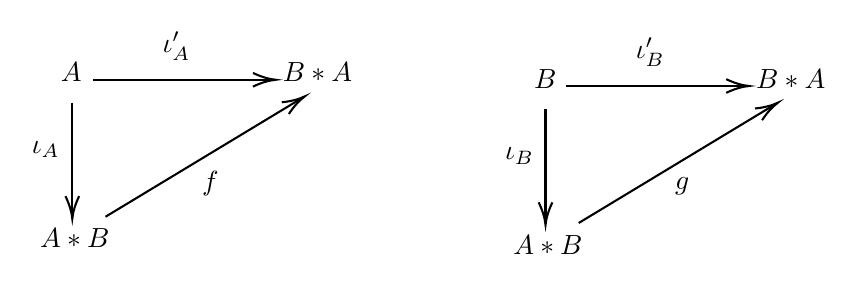
\begin{tikzpicture}[x=0.75pt,y=0.75pt,yscale=-1,xscale=1]
%uncomment if require: \path (0,476); %set diagram left start at 0, and has height of 476

%Straight Lines [id:da51308687576244] 
\draw    (128,112) -- (214,112) ;
\draw [shift={(216,112)}, rotate = 180] [color={rgb, 255:red, 0; green, 0; blue, 0 }  ][line width=0.75]    (10.93,-3.29) .. controls (6.95,-1.4) and (3.31,-0.3) .. (0,0) .. controls (3.31,0.3) and (6.95,1.4) .. (10.93,3.29)   ;
%Straight Lines [id:da945734561567223] 
\draw    (118,123) -- (118,177) ;
\draw [shift={(118,179)}, rotate = 270] [color={rgb, 255:red, 0; green, 0; blue, 0 }  ][line width=0.75]    (10.93,-3.29) .. controls (6.95,-1.4) and (3.31,-0.3) .. (0,0) .. controls (3.31,0.3) and (6.95,1.4) .. (10.93,3.29)   ;
%Straight Lines [id:da6039140489558597] 
\draw    (134,178) -- (228.29,121.03) ;
\draw [shift={(230,120)}, rotate = 148.86] [color={rgb, 255:red, 0; green, 0; blue, 0 }  ][line width=0.75]    (10.93,-3.29) .. controls (6.95,-1.4) and (3.31,-0.3) .. (0,0) .. controls (3.31,0.3) and (6.95,1.4) .. (10.93,3.29)   ;
%Straight Lines [id:da8764595834730253] 
\draw    (356,115) -- (442,115) ;
\draw [shift={(444,115)}, rotate = 180] [color={rgb, 255:red, 0; green, 0; blue, 0 }  ][line width=0.75]    (10.93,-3.29) .. controls (6.95,-1.4) and (3.31,-0.3) .. (0,0) .. controls (3.31,0.3) and (6.95,1.4) .. (10.93,3.29)   ;
%Straight Lines [id:da5299342468146768] 
\draw    (346,126) -- (346,180) ;
\draw [shift={(346,182)}, rotate = 270] [color={rgb, 255:red, 0; green, 0; blue, 0 }  ][line width=0.75]    (10.93,-3.29) .. controls (6.95,-1.4) and (3.31,-0.3) .. (0,0) .. controls (3.31,0.3) and (6.95,1.4) .. (10.93,3.29)   ;
%Straight Lines [id:da1921306060851975] 
\draw    (362,181) -- (456.29,124.03) ;
\draw [shift={(458,123)}, rotate = 148.86] [color={rgb, 255:red, 0; green, 0; blue, 0 }  ][line width=0.75]    (10.93,-3.29) .. controls (6.95,-1.4) and (3.31,-0.3) .. (0,0) .. controls (3.31,0.3) and (6.95,1.4) .. (10.93,3.29)   ;

% Text Node
\draw (111,102.4) node [anchor=north west][inner sep=0.75pt]    {$A$};
% Text Node
\draw (101,182.4) node [anchor=north west][inner sep=0.75pt]    {$A*B$};
% Text Node
\draw (218,102.4) node [anchor=north west][inner sep=0.75pt]    {$B*A$};
% Text Node
\draw (97,140.4) node [anchor=north west][inner sep=0.75pt]    {$\iota _{A}$};
% Text Node
\draw (160,87.4) node [anchor=north west][inner sep=0.75pt]    {$\iota _{A}^{\prime }$};
% Text Node
\draw (179,154.4) node [anchor=north west][inner sep=0.75pt]    {$f$};
% Text Node
\draw (339,105.4) node [anchor=north west][inner sep=0.75pt]    {$B$};
% Text Node
\draw (329,185.4) node [anchor=north west][inner sep=0.75pt]    {$A*B$};
% Text Node
\draw (446,105.4) node [anchor=north west][inner sep=0.75pt]    {$B*A$};
% Text Node
\draw (325,143.4) node [anchor=north west][inner sep=0.75pt]    {$\iota _{B}$};
% Text Node
\draw (388,90.4) node [anchor=north west][inner sep=0.75pt]    {$\iota _{B}^{\prime }$};
% Text Node
\draw (407,157.4) node [anchor=north west][inner sep=0.75pt]    {$g$};


\end{tikzpicture}
\end{center}
here $\iota$ are canonical injections. Then we know that 
$$
\begin{cases}
	\iota _A=g\circ \iota _{A}^{\prime},\\
	\iota _B=g\circ \iota _{B}^{\prime},\\
\end{cases}\hspace{1em}\begin{cases}
	\iota _{A}^{\prime}=f\circ \iota _A,\\
	\iota _{B}^{\prime}=f\circ \iota _B,\\
\end{cases}
$$
hence
$$
\begin{cases}
	\iota _A=\left( g\circ f \right) \circ \iota _A,\\
	\iota _B=\left( g\circ f \right) \circ \iota _B,\\
\end{cases}
$$
therefore $g\circ f=1_{A*B}$. Note that the diagram below is also commutative: 
\begin{center}


\tikzset{every picture/.style={line width=0.75pt}} %set default line width to 0.75pt        

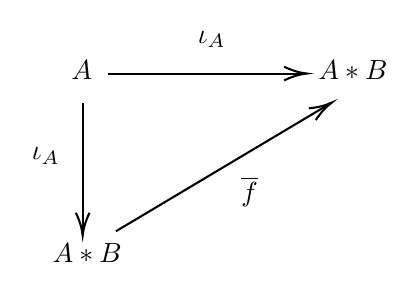
\begin{tikzpicture}[x=0.75pt,y=0.75pt,yscale=-1,xscale=1]
%uncomment if require: \path (0,476); %set diagram left start at 0, and has height of 476

%Straight Lines [id:da1882925271714635] 
\draw    (204,106) -- (298,106) ;
\draw [shift={(300,106)}, rotate = 180] [color={rgb, 255:red, 0; green, 0; blue, 0 }  ][line width=0.75]    (10.93,-3.29) .. controls (6.95,-1.4) and (3.31,-0.3) .. (0,0) .. controls (3.31,0.3) and (6.95,1.4) .. (10.93,3.29)   ;
%Straight Lines [id:da2195364554507213] 
\draw    (192,120) -- (192,182) ;
\draw [shift={(192,184)}, rotate = 270] [color={rgb, 255:red, 0; green, 0; blue, 0 }  ][line width=0.75]    (10.93,-3.29) .. controls (6.95,-1.4) and (3.31,-0.3) .. (0,0) .. controls (3.31,0.3) and (6.95,1.4) .. (10.93,3.29)   ;
%Straight Lines [id:da8375339469219252] 
\draw    (208,182) -- (310.28,121.02) ;
\draw [shift={(312,120)}, rotate = 149.2] [color={rgb, 255:red, 0; green, 0; blue, 0 }  ][line width=0.75]    (10.93,-3.29) .. controls (6.95,-1.4) and (3.31,-0.3) .. (0,0) .. controls (3.31,0.3) and (6.95,1.4) .. (10.93,3.29)   ;

% Text Node
\draw (185,98.4) node [anchor=north west][inner sep=0.75pt]    {$A$};
% Text Node
\draw (176,186.4) node [anchor=north west][inner sep=0.75pt]    {$A*B$};
% Text Node
\draw (304,98.4) node [anchor=north west][inner sep=0.75pt]    {$A*B$};
% Text Node
\draw (166,140.4) node [anchor=north west][inner sep=0.75pt]    {$\iota _{A}$};
% Text Node
\draw (246,84.4) node [anchor=north west][inner sep=0.75pt]    {$\iota _{A}$};
% Text Node
\draw (267,154.4) node [anchor=north west][inner sep=0.75pt]    {$\overline{f}$};


\end{tikzpicture}
\end{center}
hence by the uniqueness of $\overline{f}$ we know that $\overline{f}=1_{A*B}$. Similarly we may show that $\overline{g}=1_{B*A}$. Now consider the commutative diagram below: 
\begin{center}


\tikzset{every picture/.style={line width=0.75pt}} %set default line width to 0.75pt        

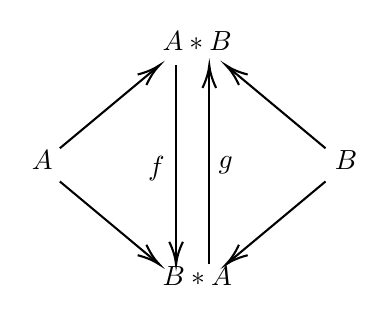
\begin{tikzpicture}[x=0.75pt,y=0.75pt,yscale=-1,xscale=1]
%uncomment if require: \path (0,476); %set diagram left start at 0, and has height of 476

%Straight Lines [id:da19202606498126973] 
\draw    (176,184) -- (222.46,145.28) ;
\draw [shift={(224,144)}, rotate = 140.19] [color={rgb, 255:red, 0; green, 0; blue, 0 }  ][line width=0.75]    (10.93,-3.29) .. controls (6.95,-1.4) and (3.31,-0.3) .. (0,0) .. controls (3.31,0.3) and (6.95,1.4) .. (10.93,3.29)   ;
%Straight Lines [id:da9962758023179532] 
\draw    (176,200) -- (222.46,238.72) ;
\draw [shift={(224,240)}, rotate = 219.81] [color={rgb, 255:red, 0; green, 0; blue, 0 }  ][line width=0.75]    (10.93,-3.29) .. controls (6.95,-1.4) and (3.31,-0.3) .. (0,0) .. controls (3.31,0.3) and (6.95,1.4) .. (10.93,3.29)   ;
%Straight Lines [id:da22458634941235944] 
\draw    (304,184) -- (257.54,145.28) ;
\draw [shift={(256,144)}, rotate = 39.81] [color={rgb, 255:red, 0; green, 0; blue, 0 }  ][line width=0.75]    (10.93,-3.29) .. controls (6.95,-1.4) and (3.31,-0.3) .. (0,0) .. controls (3.31,0.3) and (6.95,1.4) .. (10.93,3.29)   ;
%Straight Lines [id:da6914952904257381] 
\draw    (304,200) -- (257.54,238.72) ;
\draw [shift={(256,240)}, rotate = 320.19] [color={rgb, 255:red, 0; green, 0; blue, 0 }  ][line width=0.75]    (10.93,-3.29) .. controls (6.95,-1.4) and (3.31,-0.3) .. (0,0) .. controls (3.31,0.3) and (6.95,1.4) .. (10.93,3.29)   ;
%Straight Lines [id:da6281527000369735] 
\draw    (232,144) -- (232,238) ;
\draw [shift={(232,240)}, rotate = 270] [color={rgb, 255:red, 0; green, 0; blue, 0 }  ][line width=0.75]    (10.93,-3.29) .. controls (6.95,-1.4) and (3.31,-0.3) .. (0,0) .. controls (3.31,0.3) and (6.95,1.4) .. (10.93,3.29)   ;
%Straight Lines [id:da04897854339512486] 
\draw    (248,240) -- (248,146) ;
\draw [shift={(248,144)}, rotate = 90] [color={rgb, 255:red, 0; green, 0; blue, 0 }  ][line width=0.75]    (10.93,-3.29) .. controls (6.95,-1.4) and (3.31,-0.3) .. (0,0) .. controls (3.31,0.3) and (6.95,1.4) .. (10.93,3.29)   ;

% Text Node
\draw (161,183.4) node [anchor=north west][inner sep=0.75pt]    {$A$};
% Text Node
\draw (307,183.4) node [anchor=north west][inner sep=0.75pt]    {$B$};
% Text Node
\draw (224,126.4) node [anchor=north west][inner sep=0.75pt]    {$A*B$};
% Text Node
\draw (224,239.4) node [anchor=north west][inner sep=0.75pt]    {$B*A$};
% Text Node
\draw (217,186.4) node [anchor=north west][inner sep=0.75pt]    {$f$};
% Text Node
\draw (251,186.4) node [anchor=north west][inner sep=0.75pt]    {$g$};


\end{tikzpicture}
\end{center}
By $f\circ g=1_{B*A}$ and $g\circ f=1_{A*B}$ we know that there exists an isomorphism between $A*B$ and $B*A$, hence $A*B\cong B*A$. Similarly we may proof the associativity.
\end{proof}
\begin{problem}\em
If $N$ is the normal subgroup of $A*B$ generated by $A$, then $(A*B)/N\cong B$.
\end{problem}
\begin{proof}
We consider the canonical projection $\pi_A:A*B\to B$. Then it is easy to verify that $\mathrm{Ker}\pi_A=N$. Therefore by the First Isomorphism Theorem we know $(A*B)/N\cong B$.
\end{proof}
\begin{problem}\em
If $G$ and $H$ each have more than one element, then $G*H$ is an infinite group with center $\left<e\right>$.
\end{problem}
\begin{proof}
It is clear that $(ab)^n$, $n\in\mathbb{Z}$ differs since the length of them differs. Hence $G*H$ is infinite. Now we show that $Z(A*B)=\left<e\right>$. Consider $w\in A*B$. Without loss of generality we may assume $W$ ends with $a_r$, which is a word in $A$. Therefore for all $b\in B$, clearly $bw\ne wb$ since $bw$ ends with a word in $A$, but $wb$ ends with a word in $B$. Since this is true for all nontrivial $w\in A*B$, we conclude that $Z(A*B)=\left<e\right>$.
\end{proof}
\begin{problem}\em
A free group is a free product of infinite cyclic groups.
\end{problem}
\begin{proof}
Let $F$ be a free group on $X$. Then $F=\left<X\right>$. Hence $F$ is the free product ${\prod}^*_{x\in X}\left<x\right>$, which is a free product of infinite cyclic groups.
\end{proof}